\documentclass[twoside]{book}

% Packages required by doxygen
\usepackage{fixltx2e}
\usepackage{calc}
\usepackage{doxygen}
\usepackage[export]{adjustbox} % also loads graphicx
\usepackage{graphicx}
\usepackage[utf8]{inputenc}
\usepackage{makeidx}
\usepackage{multicol}
\usepackage{multirow}
\PassOptionsToPackage{warn}{textcomp}
\usepackage{textcomp}
\usepackage[nointegrals]{wasysym}
\usepackage[table]{xcolor}

% Font selection
\usepackage[T1]{fontenc}
\usepackage[scaled=.90]{helvet}
\usepackage{courier}
\usepackage{amssymb}
\usepackage{sectsty}
\renewcommand{\familydefault}{\sfdefault}
\allsectionsfont{%
  \fontseries{bc}\selectfont%
  \color{darkgray}%
}
\renewcommand{\DoxyLabelFont}{%
  \fontseries{bc}\selectfont%
  \color{darkgray}%
}
\newcommand{\+}{\discretionary{\mbox{\scriptsize$\hookleftarrow$}}{}{}}

% Page & text layout
\usepackage{geometry}
\geometry{%
  a4paper,%
  top=2.5cm,%
  bottom=2.5cm,%
  left=2.5cm,%
  right=2.5cm%
}
\tolerance=750
\hfuzz=15pt
\hbadness=750
\setlength{\emergencystretch}{15pt}
\setlength{\parindent}{0cm}
\setlength{\parskip}{3ex plus 2ex minus 2ex}
\makeatletter
\renewcommand{\paragraph}{%
  \@startsection{paragraph}{4}{0ex}{-1.0ex}{1.0ex}{%
    \normalfont\normalsize\bfseries\SS@parafont%
  }%
}
\renewcommand{\subparagraph}{%
  \@startsection{subparagraph}{5}{0ex}{-1.0ex}{1.0ex}{%
    \normalfont\normalsize\bfseries\SS@subparafont%
  }%
}
\makeatother

% Headers & footers
\usepackage{fancyhdr}
\pagestyle{fancyplain}
\fancyhead[LE]{\fancyplain{}{\bfseries\thepage}}
\fancyhead[CE]{\fancyplain{}{}}
\fancyhead[RE]{\fancyplain{}{\bfseries\leftmark}}
\fancyhead[LO]{\fancyplain{}{\bfseries\rightmark}}
\fancyhead[CO]{\fancyplain{}{}}
\fancyhead[RO]{\fancyplain{}{\bfseries\thepage}}
\fancyfoot[LE]{\fancyplain{}{}}
\fancyfoot[CE]{\fancyplain{}{}}
\fancyfoot[RE]{\fancyplain{}{\bfseries\scriptsize Generated by Doxygen }}
\fancyfoot[LO]{\fancyplain{}{\bfseries\scriptsize Generated by Doxygen }}
\fancyfoot[CO]{\fancyplain{}{}}
\fancyfoot[RO]{\fancyplain{}{}}
\renewcommand{\footrulewidth}{0.4pt}
\renewcommand{\chaptermark}[1]{%
  \markboth{#1}{}%
}
\renewcommand{\sectionmark}[1]{%
  \markright{\thesection\ #1}%
}

% Indices & bibliography
\usepackage{natbib}
\usepackage[titles]{tocloft}
\setcounter{tocdepth}{3}
\setcounter{secnumdepth}{5}
\makeindex

% Hyperlinks (required, but should be loaded last)
\usepackage{ifpdf}
\ifpdf
  \usepackage[pdftex,pagebackref=true]{hyperref}
\else
  \usepackage[ps2pdf,pagebackref=true]{hyperref}
\fi
\hypersetup{%
  colorlinks=true,%
  linkcolor=blue,%
  citecolor=blue,%
  unicode%
}

% Custom commands
\newcommand{\clearemptydoublepage}{%
  \newpage{\pagestyle{empty}\cleardoublepage}%
}

\usepackage{caption}
\captionsetup{labelsep=space,justification=centering,font={bf},singlelinecheck=off,skip=4pt,position=top}

%===== C O N T E N T S =====

\begin{document}

% Titlepage & ToC
\hypersetup{pageanchor=false,
             bookmarksnumbered=true,
             pdfencoding=unicode
            }
\pagenumbering{roman}
\begin{titlepage}
\vspace*{7cm}
\begin{center}%
{\Large nfccontroler library }\\
\vspace*{1cm}
{\large Generated by Doxygen 1.8.11}\\
\end{center}
\end{titlepage}
\clearemptydoublepage
\tableofcontents
\clearemptydoublepage
\pagenumbering{arabic}
\hypersetup{pageanchor=true}

%--- Begin generated contents ---
\chapter{Main Page}
\label{index}\hypertarget{index}{}nfccontroler library

\begin{DoxyAuthor}{Author}
David de Jong (\href{mailto:marijn_david@hotmail.com}{\tt marijn\+\_\+david@hotmail.\+com}) 
\end{DoxyAuthor}
\begin{DoxyVersion}{Version}
1.\+0 (last modified 2016-\/06-\/11) 
\end{DoxyVersion}
\begin{DoxyCopyright}{Copyright}
Published under the boost licence.
\end{DoxyCopyright}
nfccontroller is a library for the use of controlling N\+FC reader microcontrollers. This library was made as part of the V1\+I\+P\+A\+S-\/\+TI course at the Hogeschool Utrecht. This library is intended to be used with Hwlib ((c) Wouter van Ooien (\href{mailto:wouter@voti.nl}{\tt wouter@voti.\+nl}). The language is C++ from the 2011 standard.

This library currently supports the following N\+FC microcontrollers\+:
\begin{DoxyItemize}
\item R\+F\+ID -\/ \hyperlink{class_r_c522}{R\+C522}
\end{DoxyItemize}

And the following card protocols\+:
\begin{DoxyItemize}
\item Mifare Classic. which uses parts of the (I\+S\+O/\+I\+EC 14443-\/3 Type A) standard.
\end{DoxyItemize}

The library is used by including either \hyperlink{nfccontroler__all_8hpp_source}{nfccontroler\+\_\+all.\+hpp} or, preferably, by including the N\+FC chip and card protocol you want to use.

Naming convention\+:


\begin{DoxyItemize}
\item Functions that have \textquotesingle{}register\textquotesingle{} as part of their name are used to manipulate the internal registers of the N\+FC microcontroller. These functions are low level and O\+N\+LY meant to be used if the user has I\+N\+T\+I\+M\+A\+TE K\+N\+O\+W\+L\+E\+D\+GE of the internal workings of the microcontroller in question. These functions set, get or alter the variables currently available in the register. Using such a function twice in the same context will not alter the effect. The only exception to this is the F\+I\+F\+O-\/buffer because this register is used to store data.
\item Functions with more descriptive names such as \textquotesingle{}antenna\+On\textquotesingle{} or \textquotesingle{}calc\+C\+RC\textquotesingle{} are used to perform standard operations of the microcontroller. Caution is advised since some if these functions require advanced knowledge of the internal workings of the card protocol or microcontroller.
\item Functions that contain the words \textquotesingle{}block\textquotesingle{} or \textquotesingle{}sector\textquotesingle{} as part of their name are functions that deal with sending and receiving information to the card in coherence with the used protocol. These functions are the top level of the library and are intended for general use.
\end{DoxyItemize}

Usability\+:


\begin{DoxyItemize}
\item The top level of this library is meant to be usable and understandable by people with a basic understanding of C++ and the card protocol they are using.
\item The low level functions are meant to be usable and understandable by people with a more advanced understanding of the microcontrollers functionality. 
\end{DoxyItemize}
\chapter{To do list}
\label{todo}
\hypertarget{todo}{}
Future expansions\+:
\begin{DoxyItemize}
\item Cascade functionality for the anti-\/collision loop (select\+Card) to allow multiple cards in the EM field.
\item Functionality to change the Security bytes of a sector.
\item Improved C\+RC handling so C\+RC can be added even if the amount of bytes sent fills up the buffer.
\item Improved bit wrapping functionality for the Communicate\+N\+FC function.
\item Variable length matrix support for use with different card standards.
\item Support for other M\+I\+F\+A\+RE protocols.
\item Support for non M\+I\+F\+A\+RE protocols.
\item Support for other N\+FC microcontrollers. 
\end{DoxyItemize}
\chapter{Hierarchical Index}
\section{Class Hierarchy}
This inheritance list is sorted roughly, but not completely, alphabetically\+:\begin{DoxyCompactList}
\item \contentsline{section}{hwlib\+:\+:\+\_\+boolalpha}{\pageref{structhwlib_1_1__boolalpha}}{}
\item \contentsline{section}{hwlib\+:\+:\+\_\+flush}{\pageref{structhwlib_1_1__flush}}{}
\item \contentsline{section}{hwlib\+:\+:\+\_\+left}{\pageref{structhwlib_1_1__left}}{}
\item \contentsline{section}{hwlib\+:\+:\+\_\+right}{\pageref{structhwlib_1_1__right}}{}
\item \contentsline{section}{hwlib\+:\+:\+\_\+setbase}{\pageref{structhwlib_1_1__setbase}}{}
\item \contentsline{section}{hwlib\+:\+:\+\_\+showbase}{\pageref{structhwlib_1_1__showbase}}{}
\item \contentsline{section}{hwlib\+:\+:\+\_\+showpos}{\pageref{structhwlib_1_1__showpos}}{}
\item \contentsline{section}{hwlib\+:\+:adc}{\pageref{classhwlib_1_1adc}}{}
\begin{DoxyCompactList}
\item \contentsline{section}{db103\+:\+:pin\+\_\+adc}{\pageref{classdb103_1_1pin__adc}}{}
\end{DoxyCompactList}
\item \contentsline{section}{hwlib\+:\+:color}{\pageref{classhwlib_1_1color}}{}
\item \contentsline{section}{hwlib\+:\+:dac}{\pageref{classhwlib_1_1dac}}{}
\item \contentsline{section}{hwlib\+:\+:drawable}{\pageref{classhwlib_1_1drawable}}{}
\begin{DoxyCompactList}
\item \contentsline{section}{hwlib\+:\+:circle}{\pageref{classhwlib_1_1circle}}{}
\item \contentsline{section}{hwlib\+:\+:line}{\pageref{classhwlib_1_1line}}{}
\end{DoxyCompactList}
\item \contentsline{section}{hwlib\+:\+:i2c\+\_\+bus}{\pageref{classhwlib_1_1i2c__bus}}{}
\begin{DoxyCompactList}
\item \contentsline{section}{hwlib\+:\+:i2c\+\_\+bus\+\_\+bit\+\_\+banged\+\_\+scl\+\_\+sda}{\pageref{classhwlib_1_1i2c__bus__bit__banged__scl__sda}}{}
\end{DoxyCompactList}
\item \contentsline{section}{hwlib\+:\+:location}{\pageref{classhwlib_1_1location}}{}
\item \contentsline{section}{hwlib\+:\+:ostream}{\pageref{classhwlib_1_1ostream}}{}
\begin{DoxyCompactList}
\item \contentsline{section}{hwlib\+:\+:console}{\pageref{classhwlib_1_1console}}{}
\begin{DoxyCompactList}
\item \contentsline{section}{hwlib\+:\+:hd44780}{\pageref{classhwlib_1_1hd44780}}{}
\end{DoxyCompactList}
\end{DoxyCompactList}
\item \contentsline{section}{hwlib\+:\+:pcf8591}{\pageref{classhwlib_1_1pcf8591}}{}
\item \contentsline{section}{hwlib\+:\+:pin\+\_\+in}{\pageref{classhwlib_1_1pin__in}}{}
\begin{DoxyCompactList}
\item \contentsline{section}{db103\+:\+:pin\+\_\+in}{\pageref{classdb103_1_1pin__in}}{}
\item \contentsline{section}{hwlib\+:\+:\+\_\+pin\+\_\+in\+\_\+dummy\+\_\+class}{\pageref{classhwlib_1_1__pin__in__dummy__class}}{}
\item \contentsline{section}{uno\+:\+:pin\+\_\+in}{\pageref{classuno_1_1pin__in}}{}
\end{DoxyCompactList}
\item \contentsline{section}{hwlib\+:\+:pin\+\_\+in\+\_\+out}{\pageref{classhwlib_1_1pin__in__out}}{}
\begin{DoxyCompactList}
\item \contentsline{section}{db103\+:\+:pin\+\_\+in\+\_\+out}{\pageref{classdb103_1_1pin__in__out}}{}
\item \contentsline{section}{hwlib\+:\+:\+\_\+pin\+\_\+in\+\_\+out\+\_\+dummy\+\_\+class}{\pageref{classhwlib_1_1__pin__in__out__dummy__class}}{}
\item \contentsline{section}{uno\+:\+:pin\+\_\+in\+\_\+out}{\pageref{classuno_1_1pin__in__out}}{}
\end{DoxyCompactList}
\item \contentsline{section}{hwlib\+:\+:pin\+\_\+oc}{\pageref{classhwlib_1_1pin__oc}}{}
\begin{DoxyCompactList}
\item \contentsline{section}{db103\+:\+:pin\+\_\+oc}{\pageref{classdb103_1_1pin__oc}}{}
\item \contentsline{section}{hwlib\+:\+:\+\_\+pin\+\_\+oc\+\_\+dummy\+\_\+class}{\pageref{classhwlib_1_1__pin__oc__dummy__class}}{}
\item \contentsline{section}{uno\+:\+:pin\+\_\+oc}{\pageref{classuno_1_1pin__oc}}{}
\end{DoxyCompactList}
\item \contentsline{section}{hwlib\+:\+:pin\+\_\+out}{\pageref{classhwlib_1_1pin__out}}{}
\begin{DoxyCompactList}
\item \contentsline{section}{db103\+:\+:pin\+\_\+out}{\pageref{classdb103_1_1pin__out}}{}
\item \contentsline{section}{hwlib\+:\+:\+\_\+pin\+\_\+out\+\_\+dummy\+\_\+class}{\pageref{classhwlib_1_1__pin__out__dummy__class}}{}
\item \contentsline{section}{uno\+:\+:pin\+\_\+out}{\pageref{classuno_1_1pin__out}}{}
\end{DoxyCompactList}
\item \contentsline{section}{hwlib\+:\+:port\+\_\+in}{\pageref{classhwlib_1_1port__in}}{}
\begin{DoxyCompactList}
\item \contentsline{section}{hwlib\+:\+:port\+\_\+in\+\_\+from\+\_\+pins}{\pageref{classhwlib_1_1port__in__from__pins}}{}
\item \contentsline{section}{hwlib\+:\+:port\+\_\+in\+\_\+invert}{\pageref{classhwlib_1_1port__in__invert}}{}
\end{DoxyCompactList}
\item \contentsline{section}{hwlib\+:\+:port\+\_\+in\+\_\+out}{\pageref{classhwlib_1_1port__in__out}}{}
\begin{DoxyCompactList}
\item \contentsline{section}{hwlib\+:\+:port\+\_\+in\+\_\+out\+\_\+from\+\_\+pins}{\pageref{classhwlib_1_1port__in__out__from__pins}}{}
\item \contentsline{section}{hwlib\+:\+:port\+\_\+in\+\_\+out\+\_\+invert}{\pageref{classhwlib_1_1port__in__out__invert}}{}
\end{DoxyCompactList}
\item \contentsline{section}{hwlib\+:\+:port\+\_\+oc}{\pageref{classhwlib_1_1port__oc}}{}
\begin{DoxyCompactList}
\item \contentsline{section}{hwlib\+:\+:pcf8574a}{\pageref{classhwlib_1_1pcf8574a}}{}
\item \contentsline{section}{hwlib\+:\+:port\+\_\+oc\+\_\+invert}{\pageref{classhwlib_1_1port__oc__invert}}{}
\end{DoxyCompactList}
\item \contentsline{section}{hwlib\+:\+:port\+\_\+out}{\pageref{classhwlib_1_1port__out}}{}
\begin{DoxyCompactList}
\item \contentsline{section}{hwlib\+:\+:hc595}{\pageref{classhwlib_1_1hc595}}{}
\item \contentsline{section}{hwlib\+:\+:port\+\_\+out\+\_\+from\+\_\+pins}{\pageref{classhwlib_1_1port__out__from__pins}}{}
\item \contentsline{section}{hwlib\+:\+:port\+\_\+out\+\_\+invert}{\pageref{classhwlib_1_1port__out__invert}}{}
\end{DoxyCompactList}
\item \contentsline{section}{hwlib\+:\+:setfill}{\pageref{structhwlib_1_1setfill}}{}
\item \contentsline{section}{hwlib\+:\+:setw}{\pageref{structhwlib_1_1setw}}{}
\item \contentsline{section}{uno\+:\+:shield\+\_\+lcd\+\_\+mcufriend}{\pageref{classuno_1_1shield__lcd__mcufriend}}{}
\item \contentsline{section}{hwlib\+:\+:spi\+\_\+bus}{\pageref{classhwlib_1_1spi__bus}}{}
\begin{DoxyCompactList}
\item \contentsline{section}{hwlib\+:\+:spi\+\_\+bus\+\_\+bit\+\_\+banged\+\_\+sclk\+\_\+mosi\+\_\+miso}{\pageref{classhwlib_1_1spi__bus__bit__banged__sclk__mosi__miso}}{}
\end{DoxyCompactList}
\item \contentsline{section}{hwlib\+:\+:window}{\pageref{classhwlib_1_1window}}{}
\begin{DoxyCompactList}
\item \contentsline{section}{hwlib\+:\+:glcd\+\_\+5510}{\pageref{classhwlib_1_1glcd__5510}}{}
\item \contentsline{section}{hwlib\+:\+:glcd\+\_\+oled}{\pageref{classhwlib_1_1glcd__oled}}{}
\item \contentsline{section}{hwlib\+:\+:window\+\_\+invert}{\pageref{classhwlib_1_1window__invert}}{}
\item \contentsline{section}{hwlib\+:\+:window\+\_\+part}{\pageref{classhwlib_1_1window__part}}{}
\end{DoxyCompactList}
\end{DoxyCompactList}

\chapter{Class Index}
\section{Class List}
Here are the classes, structs, unions and interfaces with brief descriptions\+:\begin{DoxyCompactList}
\item\contentsline{section}{\hyperlink{structhwlib_1_1__boolalpha}{hwlib\+::\+\_\+boolalpha} }{\pageref{structhwlib_1_1__boolalpha}}{}
\item\contentsline{section}{\hyperlink{structhwlib_1_1__flush}{hwlib\+::\+\_\+flush} }{\pageref{structhwlib_1_1__flush}}{}
\item\contentsline{section}{\hyperlink{structhwlib_1_1__left}{hwlib\+::\+\_\+left} }{\pageref{structhwlib_1_1__left}}{}
\item\contentsline{section}{\hyperlink{classhwlib_1_1__pin__in__dummy__class}{hwlib\+::\+\_\+pin\+\_\+in\+\_\+dummy\+\_\+class} \\*Dummy (do-\/nothing) \hyperlink{classhwlib_1_1pin__in}{pin\+\_\+in} }{\pageref{classhwlib_1_1__pin__in__dummy__class}}{}
\item\contentsline{section}{\hyperlink{classhwlib_1_1__pin__in__out__dummy__class}{hwlib\+::\+\_\+pin\+\_\+in\+\_\+out\+\_\+dummy\+\_\+class} \\*Dummy (do-\/nothing) \hyperlink{classhwlib_1_1pin__in__out}{pin\+\_\+in\+\_\+out} }{\pageref{classhwlib_1_1__pin__in__out__dummy__class}}{}
\item\contentsline{section}{\hyperlink{classhwlib_1_1__pin__oc__dummy__class}{hwlib\+::\+\_\+pin\+\_\+oc\+\_\+dummy\+\_\+class} \\*Dummy (do-\/nothing) \hyperlink{classhwlib_1_1pin__oc}{pin\+\_\+oc} }{\pageref{classhwlib_1_1__pin__oc__dummy__class}}{}
\item\contentsline{section}{\hyperlink{classhwlib_1_1__pin__out__dummy__class}{hwlib\+::\+\_\+pin\+\_\+out\+\_\+dummy\+\_\+class} \\*Dummy (do-\/nothing) \hyperlink{classhwlib_1_1pin__out}{pin\+\_\+out} }{\pageref{classhwlib_1_1__pin__out__dummy__class}}{}
\item\contentsline{section}{\hyperlink{structhwlib_1_1__right}{hwlib\+::\+\_\+right} }{\pageref{structhwlib_1_1__right}}{}
\item\contentsline{section}{\hyperlink{structhwlib_1_1__setbase}{hwlib\+::\+\_\+setbase} }{\pageref{structhwlib_1_1__setbase}}{}
\item\contentsline{section}{\hyperlink{structhwlib_1_1__showbase}{hwlib\+::\+\_\+showbase} }{\pageref{structhwlib_1_1__showbase}}{}
\item\contentsline{section}{\hyperlink{structhwlib_1_1__showpos}{hwlib\+::\+\_\+showpos} }{\pageref{structhwlib_1_1__showpos}}{}
\item\contentsline{section}{\hyperlink{classhwlib_1_1adc}{hwlib\+::adc} \\*A/D input interface }{\pageref{classhwlib_1_1adc}}{}
\item\contentsline{section}{\hyperlink{classhwlib_1_1circle}{hwlib\+::circle} }{\pageref{classhwlib_1_1circle}}{}
\item\contentsline{section}{\hyperlink{classhwlib_1_1color}{hwlib\+::color} \\*Graphics color }{\pageref{classhwlib_1_1color}}{}
\item\contentsline{section}{\hyperlink{classhwlib_1_1console}{hwlib\+::console} \\*Console interface }{\pageref{classhwlib_1_1console}}{}
\item\contentsline{section}{\hyperlink{classhwlib_1_1dac}{hwlib\+::dac} \\*D/A output interface }{\pageref{classhwlib_1_1dac}}{}
\item\contentsline{section}{\hyperlink{classhwlib_1_1drawable}{hwlib\+::drawable} }{\pageref{classhwlib_1_1drawable}}{}
\item\contentsline{section}{\hyperlink{classhwlib_1_1glcd__5510}{hwlib\+::glcd\+\_\+5510} \\*Nokia 5510 B/W graphics L\+CD library }{\pageref{classhwlib_1_1glcd__5510}}{}
\item\contentsline{section}{\hyperlink{classhwlib_1_1glcd__oled}{hwlib\+::glcd\+\_\+oled} \\*Oled B/W graphics L\+CD }{\pageref{classhwlib_1_1glcd__oled}}{}
\item\contentsline{section}{\hyperlink{classhwlib_1_1hc595}{hwlib\+::hc595} \\*Hc595 8-\/bit output shift register }{\pageref{classhwlib_1_1hc595}}{}
\item\contentsline{section}{\hyperlink{classhwlib_1_1hd44780}{hwlib\+::hd44780} \\*Hd44780 character L\+CD interface }{\pageref{classhwlib_1_1hd44780}}{}
\item\contentsline{section}{\hyperlink{classhwlib_1_1i2c__bus}{hwlib\+::i2c\+\_\+bus} \\*I2c bus master interface }{\pageref{classhwlib_1_1i2c__bus}}{}
\item\contentsline{section}{\hyperlink{classhwlib_1_1i2c__bus__bit__banged__scl__sda}{hwlib\+::i2c\+\_\+bus\+\_\+bit\+\_\+banged\+\_\+scl\+\_\+sda} \\*Bit-\/banged i2c bus implementation }{\pageref{classhwlib_1_1i2c__bus__bit__banged__scl__sda}}{}
\item\contentsline{section}{\hyperlink{classhwlib_1_1line}{hwlib\+::line} }{\pageref{classhwlib_1_1line}}{}
\item\contentsline{section}{\hyperlink{classhwlib_1_1location}{hwlib\+::location} \\*Pixel coordinate }{\pageref{classhwlib_1_1location}}{}
\item\contentsline{section}{\hyperlink{classhwlib_1_1ostream}{hwlib\+::ostream} \\*Formatted character output }{\pageref{classhwlib_1_1ostream}}{}
\item\contentsline{section}{\hyperlink{classhwlib_1_1pcf8574a}{hwlib\+::pcf8574a} \\*Pcf8574a I2C I/O extender }{\pageref{classhwlib_1_1pcf8574a}}{}
\item\contentsline{section}{\hyperlink{classhwlib_1_1pcf8591}{hwlib\+::pcf8591} \\*Pcf8591 I2C A/D and D/A converter }{\pageref{classhwlib_1_1pcf8591}}{}
\item\contentsline{section}{\hyperlink{classdb103_1_1pin__adc}{db103\+::pin\+\_\+adc} }{\pageref{classdb103_1_1pin__adc}}{}
\item\contentsline{section}{\hyperlink{classdb103_1_1pin__in}{db103\+::pin\+\_\+in} \\*Pin\+\_\+in implementation for the L\+P\+C1114 }{\pageref{classdb103_1_1pin__in}}{}
\item\contentsline{section}{\hyperlink{classdue_1_1pin__in}{due\+::pin\+\_\+in} \\*Pin\+\_\+in implementation for a A\+T\+S\+A\+M3\+X8E }{\pageref{classdue_1_1pin__in}}{}
\item\contentsline{section}{\hyperlink{classuno_1_1pin__in}{uno\+::pin\+\_\+in} \\*Pin\+\_\+in implementation for a A\+T\+Mega328P }{\pageref{classuno_1_1pin__in}}{}
\item\contentsline{section}{\hyperlink{classhwlib_1_1pin__in}{hwlib\+::pin\+\_\+in} \\*Input pin interface }{\pageref{classhwlib_1_1pin__in}}{}
\item\contentsline{section}{\hyperlink{classuno_1_1pin__in__out}{uno\+::pin\+\_\+in\+\_\+out} \\*Pin\+\_\+in\+\_\+out implementation for a A\+T\+Mega328P }{\pageref{classuno_1_1pin__in__out}}{}
\item\contentsline{section}{\hyperlink{classdue_1_1pin__in__out}{due\+::pin\+\_\+in\+\_\+out} \\*Pin\+\_\+in\+\_\+out implementation for a A\+T\+S\+A\+M3\+X8E }{\pageref{classdue_1_1pin__in__out}}{}
\item\contentsline{section}{\hyperlink{classhwlib_1_1pin__in__out}{hwlib\+::pin\+\_\+in\+\_\+out} \\*Input/output pin interface }{\pageref{classhwlib_1_1pin__in__out}}{}
\item\contentsline{section}{\hyperlink{classdb103_1_1pin__in__out}{db103\+::pin\+\_\+in\+\_\+out} \\*Pin\+\_\+in\+\_\+out implementation for the L\+P\+C1114 }{\pageref{classdb103_1_1pin__in__out}}{}
\item\contentsline{section}{\hyperlink{classuno_1_1pin__oc}{uno\+::pin\+\_\+oc} \\*Pin\+\_\+oc implementation for a A\+T\+Mega328P }{\pageref{classuno_1_1pin__oc}}{}
\item\contentsline{section}{\hyperlink{classhwlib_1_1pin__oc}{hwlib\+::pin\+\_\+oc} \\*Open-\/collector input/output pin interface }{\pageref{classhwlib_1_1pin__oc}}{}
\item\contentsline{section}{\hyperlink{classdue_1_1pin__oc}{due\+::pin\+\_\+oc} \\*Pin\+\_\+oc implementation for a A\+T\+S\+A\+M3\+X8E }{\pageref{classdue_1_1pin__oc}}{}
\item\contentsline{section}{\hyperlink{classdb103_1_1pin__oc}{db103\+::pin\+\_\+oc} \\*Pin\+\_\+oc implementation for the L\+P\+C1114 }{\pageref{classdb103_1_1pin__oc}}{}
\item\contentsline{section}{\hyperlink{classdue_1_1pin__out}{due\+::pin\+\_\+out} \\*Pin\+\_\+out implementation for a A\+T\+S\+A\+M3\+X8E }{\pageref{classdue_1_1pin__out}}{}
\item\contentsline{section}{\hyperlink{classuno_1_1pin__out}{uno\+::pin\+\_\+out} \\*Pin\+\_\+out implementation for a A\+T\+Mega328P }{\pageref{classuno_1_1pin__out}}{}
\item\contentsline{section}{\hyperlink{classdb103_1_1pin__out}{db103\+::pin\+\_\+out} \\*Pin\+\_\+out implementation for the L\+P\+C1114 }{\pageref{classdb103_1_1pin__out}}{}
\item\contentsline{section}{\hyperlink{classhwlib_1_1pin__out}{hwlib\+::pin\+\_\+out} \\*Output pin interface }{\pageref{classhwlib_1_1pin__out}}{}
\item\contentsline{section}{\hyperlink{classhwlib_1_1port__in}{hwlib\+::port\+\_\+in} \\*Input port interface }{\pageref{classhwlib_1_1port__in}}{}
\item\contentsline{section}{\hyperlink{classhwlib_1_1port__in__from__pins}{hwlib\+::port\+\_\+in\+\_\+from\+\_\+pins} \\*Input port from input pins }{\pageref{classhwlib_1_1port__in__from__pins}}{}
\item\contentsline{section}{\hyperlink{classhwlib_1_1port__in__invert}{hwlib\+::port\+\_\+in\+\_\+invert} \\*Invert an input port }{\pageref{classhwlib_1_1port__in__invert}}{}
\item\contentsline{section}{\hyperlink{classhwlib_1_1port__in__out}{hwlib\+::port\+\_\+in\+\_\+out} \\*Input / output port interface }{\pageref{classhwlib_1_1port__in__out}}{}
\item\contentsline{section}{\hyperlink{classhwlib_1_1port__in__out__from__pins}{hwlib\+::port\+\_\+in\+\_\+out\+\_\+from\+\_\+pins} \\*Input/output port from input/output pins }{\pageref{classhwlib_1_1port__in__out__from__pins}}{}
\item\contentsline{section}{\hyperlink{classhwlib_1_1port__in__out__invert}{hwlib\+::port\+\_\+in\+\_\+out\+\_\+invert} \\*Invert an input/input port }{\pageref{classhwlib_1_1port__in__out__invert}}{}
\item\contentsline{section}{\hyperlink{classhwlib_1_1port__oc}{hwlib\+::port\+\_\+oc} \\*Open-\/collector interface }{\pageref{classhwlib_1_1port__oc}}{}
\item\contentsline{section}{\hyperlink{classhwlib_1_1port__oc__invert}{hwlib\+::port\+\_\+oc\+\_\+invert} \\*Invert an open-\/collector port }{\pageref{classhwlib_1_1port__oc__invert}}{}
\item\contentsline{section}{\hyperlink{classhwlib_1_1port__out}{hwlib\+::port\+\_\+out} \\*Output port interface }{\pageref{classhwlib_1_1port__out}}{}
\item\contentsline{section}{\hyperlink{classhwlib_1_1port__out__from__pins}{hwlib\+::port\+\_\+out\+\_\+from\+\_\+pins} \\*Output port from output pins }{\pageref{classhwlib_1_1port__out__from__pins}}{}
\item\contentsline{section}{\hyperlink{classhwlib_1_1port__out__invert}{hwlib\+::port\+\_\+out\+\_\+invert} \\*Invert an output port }{\pageref{classhwlib_1_1port__out__invert}}{}
\item\contentsline{section}{\hyperlink{structhwlib_1_1setfill}{hwlib\+::setfill} \\*Ostream filler character manipulator }{\pageref{structhwlib_1_1setfill}}{}
\item\contentsline{section}{\hyperlink{structhwlib_1_1setw}{hwlib\+::setw} \\*Ostream output field width manipulator }{\pageref{structhwlib_1_1setw}}{}
\item\contentsline{section}{\hyperlink{classuno_1_1shield__lcd__mcufriend}{uno\+::shield\+\_\+lcd\+\_\+mcufriend} }{\pageref{classuno_1_1shield__lcd__mcufriend}}{}
\item\contentsline{section}{\hyperlink{classhwlib_1_1spi__bus}{hwlib\+::spi\+\_\+bus} \\*Spi bus interface }{\pageref{classhwlib_1_1spi__bus}}{}
\item\contentsline{section}{\hyperlink{classhwlib_1_1spi__bus__bit__banged__sclk__mosi__miso}{hwlib\+::spi\+\_\+bus\+\_\+bit\+\_\+banged\+\_\+sclk\+\_\+mosi\+\_\+miso} \\*Bit-\/banged S\+PI bus implementation }{\pageref{classhwlib_1_1spi__bus__bit__banged__sclk__mosi__miso}}{}
\item\contentsline{section}{\hyperlink{classhwlib_1_1window}{hwlib\+::window} \\*Graphics windows }{\pageref{classhwlib_1_1window}}{}
\item\contentsline{section}{\hyperlink{classhwlib_1_1window__invert}{hwlib\+::window\+\_\+invert} \\*Window\+\_\+invert (invert writes to a window) }{\pageref{classhwlib_1_1window__invert}}{}
\item\contentsline{section}{\hyperlink{classhwlib_1_1window__part}{hwlib\+::window\+\_\+part} \\*Window\+\_\+part (subwindow of a larger window) }{\pageref{classhwlib_1_1window__part}}{}
\end{DoxyCompactList}

\chapter{File Index}
\section{File List}
Here is a list of all documented files with brief descriptions\+:\begin{DoxyCompactList}
\item\contentsline{section}{\hyperlink{hwlib-adc_8hpp}{hwlib-\/adc.\+hpp} }{\pageref{hwlib-adc_8hpp}}{}
\item\contentsline{section}{{\bfseries hwlib-\/all.\+hpp} }{\pageref{hwlib-all_8hpp}}{}
\item\contentsline{section}{\hyperlink{hwlib-console_8hpp}{hwlib-\/console.\+hpp} }{\pageref{hwlib-console_8hpp}}{}
\item\contentsline{section}{\hyperlink{hwlib-dac_8hpp}{hwlib-\/dac.\+hpp} }{\pageref{hwlib-dac_8hpp}}{}
\item\contentsline{section}{\hyperlink{hwlib-db103_8hpp}{hwlib-\/db103.\+hpp} }{\pageref{hwlib-db103_8hpp}}{}
\item\contentsline{section}{\hyperlink{hwlib-defines_8hpp}{hwlib-\/defines.\+hpp} }{\pageref{hwlib-defines_8hpp}}{}
\item\contentsline{section}{\hyperlink{hwlib-demo_8hpp}{hwlib-\/demo.\+hpp} }{\pageref{hwlib-demo_8hpp}}{}
\item\contentsline{section}{\hyperlink{hwlib-doxygen_8hpp}{hwlib-\/doxygen.\+hpp} }{\pageref{hwlib-doxygen_8hpp}}{}
\item\contentsline{section}{\hyperlink{hwlib-due_8hpp}{hwlib-\/due.\+hpp} }{\pageref{hwlib-due_8hpp}}{}
\item\contentsline{section}{\hyperlink{hwlib-glcd-5510_8hpp}{hwlib-\/glcd-\/5510.\+hpp} }{\pageref{hwlib-glcd-5510_8hpp}}{}
\item\contentsline{section}{\hyperlink{hwlib-glcd-oled_8hpp}{hwlib-\/glcd-\/oled.\+hpp} }{\pageref{hwlib-glcd-oled_8hpp}}{}
\item\contentsline{section}{\hyperlink{hwlib-graphics_8hpp}{hwlib-\/graphics.\+hpp} }{\pageref{hwlib-graphics_8hpp}}{}
\item\contentsline{section}{\hyperlink{hwlib-hc595_8hpp}{hwlib-\/hc595.\+hpp} }{\pageref{hwlib-hc595_8hpp}}{}
\item\contentsline{section}{\hyperlink{hwlib-hd44780_8hpp}{hwlib-\/hd44780.\+hpp} }{\pageref{hwlib-hd44780_8hpp}}{}
\item\contentsline{section}{\hyperlink{hwlib-i2c_8hpp}{hwlib-\/i2c.\+hpp} }{\pageref{hwlib-i2c_8hpp}}{}
\item\contentsline{section}{\hyperlink{hwlib-ostream_8hpp}{hwlib-\/ostream.\+hpp} }{\pageref{hwlib-ostream_8hpp}}{}
\item\contentsline{section}{\hyperlink{hwlib-panic_8hpp}{hwlib-\/panic.\+hpp} }{\pageref{hwlib-panic_8hpp}}{}
\item\contentsline{section}{\hyperlink{hwlib-pcf8574a_8hpp}{hwlib-\/pcf8574a.\+hpp} }{\pageref{hwlib-pcf8574a_8hpp}}{}
\item\contentsline{section}{\hyperlink{hwlib-pcf8591_8hpp}{hwlib-\/pcf8591.\+hpp} }{\pageref{hwlib-pcf8591_8hpp}}{}
\item\contentsline{section}{{\bfseries hwlib-\/pi.\+hpp} }{\pageref{hwlib-pi_8hpp}}{}
\item\contentsline{section}{\hyperlink{hwlib-pin-dummies_8hpp}{hwlib-\/pin-\/dummies.\+hpp} }{\pageref{hwlib-pin-dummies_8hpp}}{}
\item\contentsline{section}{\hyperlink{hwlib-pin_8hpp}{hwlib-\/pin.\+hpp} }{\pageref{hwlib-pin_8hpp}}{}
\item\contentsline{section}{\hyperlink{hwlib-port_8hpp}{hwlib-\/port.\+hpp} }{\pageref{hwlib-port_8hpp}}{}
\item\contentsline{section}{\hyperlink{hwlib-spi_8hpp}{hwlib-\/spi.\+hpp} }{\pageref{hwlib-spi_8hpp}}{}
\item\contentsline{section}{\hyperlink{hwlib-uno_8hpp}{hwlib-\/uno.\+hpp} }{\pageref{hwlib-uno_8hpp}}{}
\item\contentsline{section}{\hyperlink{hwlib-wait_8hpp}{hwlib-\/wait.\+hpp} }{\pageref{hwlib-wait_8hpp}}{}
\item\contentsline{section}{{\bfseries hwlib.\+hpp} }{\pageref{hwlib_8hpp}}{}
\end{DoxyCompactList}

\chapter{Class Documentation}
\hypertarget{class_mifare___classic}{}\section{Mifare\+\_\+\+Classic Class Reference}
\label{class_mifare___classic}\index{Mifare\+\_\+\+Classic@{Mifare\+\_\+\+Classic}}


{\ttfamily \#include $<$Mifare\+\_\+\+Classic.\+hpp$>$}

Inheritance diagram for Mifare\+\_\+\+Classic\+:\begin{figure}[H]
\begin{center}
\leavevmode
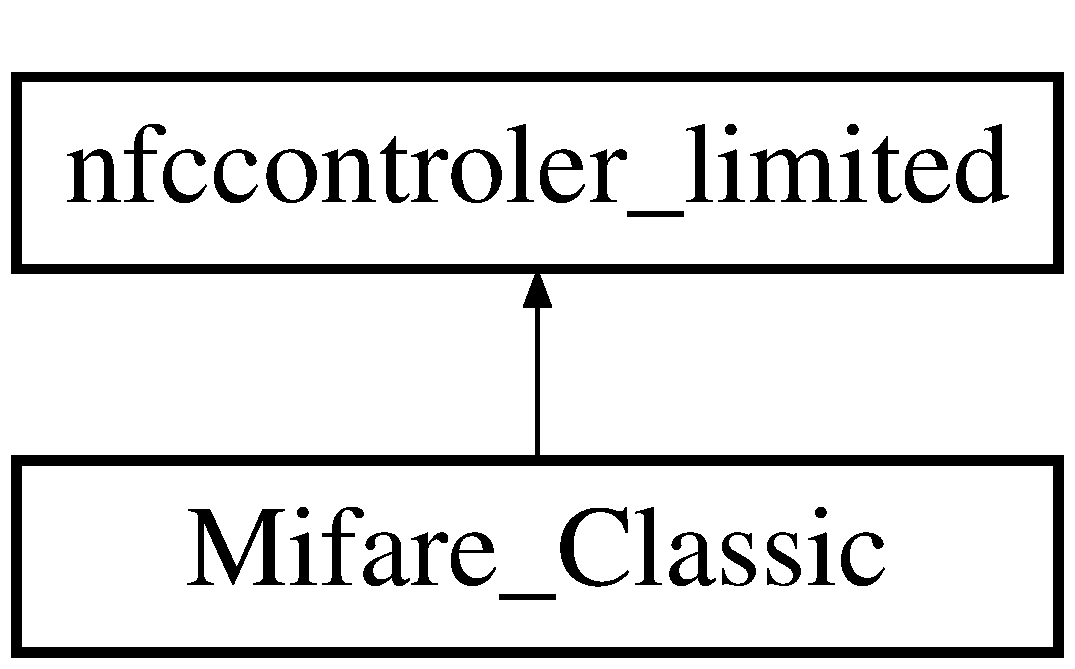
\includegraphics[height=2.000000cm]{class_mifare___classic}
\end{center}
\end{figure}
\subsection*{Public Member Functions}
\begin{DoxyCompactItemize}
\item 
\hyperlink{class_mifare___classic_a91dc3f7490d536582dd5e584cbd6ed58}{Mifare\+\_\+\+Classic} (\hyperlink{classnfccontroler__limited}{nfccontroler\+\_\+limited} \&slave)
\item 
bool \hyperlink{class_mifare___classic_ac35863ec691f0a118156bea44c4cd7a7}{trancieve\+Data} (const byte $\ast$data\+\_\+in, const int data\+\_\+in\+\_\+lenght, byte $\ast$data\+\_\+out, int $\ast$data\+\_\+out\+\_\+lenght, bool crc=false, bool Bitwraping=false) override\hypertarget{class_mifare___classic_ac35863ec691f0a118156bea44c4cd7a7}{}\label{class_mifare___classic_ac35863ec691f0a118156bea44c4cd7a7}

\begin{DoxyCompactList}\small\item\em I\+N\+T\+E\+R\+N\+AL \end{DoxyCompactList}\item 
bool {\bfseries authent\+Card} (const byte $\ast$data\+\_\+in, const int data\+\_\+in\+\_\+lenght)\hypertarget{class_mifare___classic_aa39b8fbbb2b8a66f062c02a94a43c814}{}\label{class_mifare___classic_aa39b8fbbb2b8a66f062c02a94a43c814}

\item 
void \hyperlink{class_mifare___classic_a9377d560c083320ad3b605df464a29e4}{check\+Erro\+And\+Irq} (byte $\ast$result) override
\item 
bool \hyperlink{class_mifare___classic_ae02721fc8b9268e93778fdc47d06d162}{is\+Card} (byte $\ast$cardtype) override
\item 
bool \hyperlink{class_mifare___classic_aaa549c00df8619bb2f5a96bba093f005}{select\+Card} (byte $\ast$Cardserial) override
\item 
bool \hyperlink{class_mifare___classic_a2e79d1842e44e1600f59fdfba4b22470}{authenticate\+Sector} (byte typekey, byte $\ast$block\+\_\+address, byte $\ast$key, byte $\ast$Cardserial) override
\item 
bool \hyperlink{class_mifare___classic_a6401f278760213b5c53e3c41aa5b0c98}{read\+Block} (byte block\+\_\+address, byte $\ast$data\+\_\+out) override
\item 
bool \hyperlink{class_mifare___classic_a7caca9ec9a0cdc116f8056753ecc438c}{read\+Sector} (const int sectorsize, byte($\ast$sector\+\_\+out)\mbox{[}16\mbox{]}, byte typekey, byte $\ast$first\+\_\+block\+\_\+in\+\_\+sector, byte $\ast$key, byte $\ast$Cardserial) override
\item 
bool \hyperlink{class_mifare___classic_adb793958d3f2601d336165e383a456f6}{write\+Block} (const byte block\+\_\+address, const byte $\ast$data\+\_\+in, const int lenght) override
\item 
bool \hyperlink{class_mifare___classic_a127803e07c148fe8d447a00e28be4a90}{write\+Sector} (const int sectorsize, byte($\ast$sector\+\_\+in)\mbox{[}16\mbox{]}, byte typekey, byte $\ast$first\+\_\+block\+\_\+in\+\_\+sector, byte $\ast$key, byte $\ast$Cardserial) override
\item 
bool {\bfseries calculate\+C\+RC} (const byte $\ast$data, const int length, byte $\ast$result)\hypertarget{class_mifare___classic_a915b02fa2f126741de96ce6224503ff6}{}\label{class_mifare___classic_a915b02fa2f126741de96ce6224503ff6}

\end{DoxyCompactItemize}


\subsection{Detailed Description}
Implementation of the card protocol functions for the M\+I\+F\+A\+R\+E-\/classic protocol.

This class contains the protocol specific implementation for communicating with M\+I\+F\+A\+R\+E-\/classic N\+FC cards. This class follows the Decorator type of datastructure. 

\subsection{Constructor \& Destructor Documentation}
\index{Mifare\+\_\+\+Classic@{Mifare\+\_\+\+Classic}!Mifare\+\_\+\+Classic@{Mifare\+\_\+\+Classic}}
\index{Mifare\+\_\+\+Classic@{Mifare\+\_\+\+Classic}!Mifare\+\_\+\+Classic@{Mifare\+\_\+\+Classic}}
\subsubsection[{\texorpdfstring{Mifare\+\_\+\+Classic(nfccontroler\+\_\+limited \&slave)}{Mifare_Classic(nfccontroler_limited &slave)}}]{\setlength{\rightskip}{0pt plus 5cm}Mifare\+\_\+\+Classic\+::\+Mifare\+\_\+\+Classic (
\begin{DoxyParamCaption}
\item[{{\bf nfccontroler\+\_\+limited} \&}]{slave}
\end{DoxyParamCaption}
)\hspace{0.3cm}{\ttfamily [inline]}}\hypertarget{class_mifare___classic_a91dc3f7490d536582dd5e584cbd6ed58}{}\label{class_mifare___classic_a91dc3f7490d536582dd5e584cbd6ed58}
Constructor for the M\+I\+F\+A\+R\+E-\/classic protocol decorator.

The constructor uses a microcontroler object (slave) to add protocol specific implementation functionality. 

\subsection{Member Function Documentation}
\index{Mifare\+\_\+\+Classic@{Mifare\+\_\+\+Classic}!authenticate\+Sector@{authenticate\+Sector}}
\index{authenticate\+Sector@{authenticate\+Sector}!Mifare\+\_\+\+Classic@{Mifare\+\_\+\+Classic}}
\subsubsection[{\texorpdfstring{authenticate\+Sector(byte typekey, byte $\ast$block\+\_\+address, byte $\ast$key, byte $\ast$\+Cardserial) override}{authenticateSector(byte typekey, byte *block_address, byte *key, byte *Cardserial) override}}]{\setlength{\rightskip}{0pt plus 5cm}bool Mifare\+\_\+\+Classic\+::authenticate\+Sector (
\begin{DoxyParamCaption}
\item[{byte}]{typekey, }
\item[{byte $\ast$}]{block\+\_\+address, }
\item[{byte $\ast$}]{key, }
\item[{byte $\ast$}]{Cardserial}
\end{DoxyParamCaption}
)\hspace{0.3cm}{\ttfamily [inline]}, {\ttfamily [override]}, {\ttfamily [virtual]}}\hypertarget{class_mifare___classic_a2e79d1842e44e1600f59fdfba4b22470}{}\label{class_mifare___classic_a2e79d1842e44e1600f59fdfba4b22470}
Function for authenticating access to a sector.

This function grants access to the specified sector of the card. The typekey parameter is used to specify which key is used for authentication. The block\+\_\+address parameter is used to select which sector is authenticated for. The key parameter is used to provide they key in byte array form to the specified sector. Any block in a sector may be targeted for authentication and will grant access to all blocks in that sector. This function returns true after successful authentication. 

Implements \hyperlink{classnfccontroler__limited_a4eec4cf702e4c0062c33657e81a2069f}{nfccontroler\+\_\+limited}.

\index{Mifare\+\_\+\+Classic@{Mifare\+\_\+\+Classic}!check\+Erro\+And\+Irq@{check\+Erro\+And\+Irq}}
\index{check\+Erro\+And\+Irq@{check\+Erro\+And\+Irq}!Mifare\+\_\+\+Classic@{Mifare\+\_\+\+Classic}}
\subsubsection[{\texorpdfstring{check\+Erro\+And\+Irq(byte $\ast$result) override}{checkErroAndIrq(byte *result) override}}]{\setlength{\rightskip}{0pt plus 5cm}void Mifare\+\_\+\+Classic\+::check\+Erro\+And\+Irq (
\begin{DoxyParamCaption}
\item[{byte $\ast$}]{result}
\end{DoxyParamCaption}
)\hspace{0.3cm}{\ttfamily [inline]}, {\ttfamily [override]}, {\ttfamily [virtual]}}\hypertarget{class_mifare___classic_a9377d560c083320ad3b605df464a29e4}{}\label{class_mifare___classic_a9377d560c083320ad3b605df464a29e4}
Function checking the error and I\+RQ results after sending or receiving data.

This function inserts the status of the registers in a byte array that is given to the function as a parameter.

The use function requires knowledge of how the chip returns these results. 

Implements \hyperlink{classnfccontroler__limited_a97f279888626df09059338d149a3dcf1}{nfccontroler\+\_\+limited}.

\index{Mifare\+\_\+\+Classic@{Mifare\+\_\+\+Classic}!is\+Card@{is\+Card}}
\index{is\+Card@{is\+Card}!Mifare\+\_\+\+Classic@{Mifare\+\_\+\+Classic}}
\subsubsection[{\texorpdfstring{is\+Card(byte $\ast$cardtype) override}{isCard(byte *cardtype) override}}]{\setlength{\rightskip}{0pt plus 5cm}bool Mifare\+\_\+\+Classic\+::is\+Card (
\begin{DoxyParamCaption}
\item[{byte $\ast$}]{cardtype}
\end{DoxyParamCaption}
)\hspace{0.3cm}{\ttfamily [inline]}, {\ttfamily [override]}, {\ttfamily [virtual]}}\hypertarget{class_mifare___classic_ae02721fc8b9268e93778fdc47d06d162}{}\label{class_mifare___classic_ae02721fc8b9268e93778fdc47d06d162}
Function for detecting if a card is in the EM field.

This function constantly polls for a card in the EM field When a card responds it inserts the response (Sak) in the cardtype byte array. This response can be used to identify the type of card. Before a card responds to this function it will not respond to any other command. It is currently not supported to have multiple cards in the EM field at the same time. Function will return true on successful detection of a card. 

Implements \hyperlink{classnfccontroler__limited_ae1e689d34ba8bcd933c696b3f852dad6}{nfccontroler\+\_\+limited}.

\index{Mifare\+\_\+\+Classic@{Mifare\+\_\+\+Classic}!read\+Block@{read\+Block}}
\index{read\+Block@{read\+Block}!Mifare\+\_\+\+Classic@{Mifare\+\_\+\+Classic}}
\subsubsection[{\texorpdfstring{read\+Block(byte block\+\_\+address, byte $\ast$data\+\_\+out) override}{readBlock(byte block_address, byte *data_out) override}}]{\setlength{\rightskip}{0pt plus 5cm}bool Mifare\+\_\+\+Classic\+::read\+Block (
\begin{DoxyParamCaption}
\item[{byte}]{block\+\_\+address, }
\item[{byte $\ast$}]{data\+\_\+out}
\end{DoxyParamCaption}
)\hspace{0.3cm}{\ttfamily [inline]}, {\ttfamily [override]}, {\ttfamily [virtual]}}\hypertarget{class_mifare___classic_a6401f278760213b5c53e3c41aa5b0c98}{}\label{class_mifare___classic_a6401f278760213b5c53e3c41aa5b0c98}
Function for reading a block of data from the card.

This function reads data from a single block of data inside the card. After reading the data it inserts this in the data\+\_\+out array parameter. It is required to authenticate for the sector that the block resides in before attempting to read. Upon successful reading of data this function returns true. 

Implements \hyperlink{classnfccontroler__limited_a5a8f607de57023a90962f6ac4fa2b5f1}{nfccontroler\+\_\+limited}.

\index{Mifare\+\_\+\+Classic@{Mifare\+\_\+\+Classic}!read\+Sector@{read\+Sector}}
\index{read\+Sector@{read\+Sector}!Mifare\+\_\+\+Classic@{Mifare\+\_\+\+Classic}}
\subsubsection[{\texorpdfstring{read\+Sector(const int sectorsize, byte($\ast$sector\+\_\+out)[16], byte typekey, byte $\ast$first\+\_\+block\+\_\+in\+\_\+sector, byte $\ast$key, byte $\ast$\+Cardserial) override}{readSector(const int sectorsize, byte(*sector_out)[16], byte typekey, byte *first_block_in_sector, byte *key, byte *Cardserial) override}}]{\setlength{\rightskip}{0pt plus 5cm}bool Mifare\+\_\+\+Classic\+::read\+Sector (
\begin{DoxyParamCaption}
\item[{const int}]{sectorsize, }
\item[{byte($\ast$)}]{sector\+\_\+out\mbox{[}16\mbox{]}, }
\item[{byte}]{typekey, }
\item[{byte $\ast$}]{first\+\_\+block\+\_\+in\+\_\+sector, }
\item[{byte $\ast$}]{key, }
\item[{byte $\ast$}]{Cardserial}
\end{DoxyParamCaption}
)\hspace{0.3cm}{\ttfamily [inline]}, {\ttfamily [override]}, {\ttfamily [virtual]}}\hypertarget{class_mifare___classic_a7caca9ec9a0cdc116f8056753ecc438c}{}\label{class_mifare___classic_a7caca9ec9a0cdc116f8056753ecc438c}
Function for reading an entire sector of data from the card.

This function reads an entire sector of data. After reading the data it inserts this in the sector\+\_\+out 2d matrix parameter. Authentication is built in for this function. The typekey parameter is used to specify which key is used for authentication. The first\+\_\+block\+\_\+in\+\_\+sector parameter is used to select which sector is authenticated for. The key parameter is used to provide they key in byte array form to the specified sector. Upon successful reading of the sector this function returns true. 

Implements \hyperlink{classnfccontroler__limited_a70d6de379a501af2272da775c5d27c9e}{nfccontroler\+\_\+limited}.

\index{Mifare\+\_\+\+Classic@{Mifare\+\_\+\+Classic}!select\+Card@{select\+Card}}
\index{select\+Card@{select\+Card}!Mifare\+\_\+\+Classic@{Mifare\+\_\+\+Classic}}
\subsubsection[{\texorpdfstring{select\+Card(byte $\ast$\+Cardserial) override}{selectCard(byte *Cardserial) override}}]{\setlength{\rightskip}{0pt plus 5cm}bool Mifare\+\_\+\+Classic\+::select\+Card (
\begin{DoxyParamCaption}
\item[{byte $\ast$}]{Cardserial}
\end{DoxyParamCaption}
)\hspace{0.3cm}{\ttfamily [inline]}, {\ttfamily [override]}, {\ttfamily [virtual]}}\hypertarget{class_mifare___classic_aaa549c00df8619bb2f5a96bba093f005}{}\label{class_mifare___classic_aaa549c00df8619bb2f5a96bba093f005}
Function for the selection of the card.

This function requests the U\+ID (Unique Identifier) from the card and then uses the U\+ID to select the card. It inserts the U\+ID into the Cardserial array. When a card has been successfully selected its U\+ID can be used to send other data and commands towards the card. This function returns true after the successful selection of a card. 

Implements \hyperlink{classnfccontroler__limited_a195f3de8d1529e00998f60ddf8058f6b}{nfccontroler\+\_\+limited}.

\index{Mifare\+\_\+\+Classic@{Mifare\+\_\+\+Classic}!write\+Block@{write\+Block}}
\index{write\+Block@{write\+Block}!Mifare\+\_\+\+Classic@{Mifare\+\_\+\+Classic}}
\subsubsection[{\texorpdfstring{write\+Block(const byte block\+\_\+address, const byte $\ast$data\+\_\+in, const int lenght) override}{writeBlock(const byte block_address, const byte *data_in, const int lenght) override}}]{\setlength{\rightskip}{0pt plus 5cm}bool Mifare\+\_\+\+Classic\+::write\+Block (
\begin{DoxyParamCaption}
\item[{const byte}]{block\+\_\+address, }
\item[{const byte $\ast$}]{data\+\_\+in, }
\item[{const int}]{lenght}
\end{DoxyParamCaption}
)\hspace{0.3cm}{\ttfamily [inline]}, {\ttfamily [override]}, {\ttfamily [virtual]}}\hypertarget{class_mifare___classic_adb793958d3f2601d336165e383a456f6}{}\label{class_mifare___classic_adb793958d3f2601d336165e383a456f6}
Function for writing a block of data to the card.

This function writes data to a single block of data inside the card. The parameter data\+\_\+in is used to provide the data to write in byte array form. The data given to the function is appended with zeroes so a full block is always written. It is required to authenticate for the sector that the block resides in before attempting to write. Upon successful writing of data this function returns true. 

Implements \hyperlink{classnfccontroler__limited_aeeeb82c8b45881239c7b2d9b4bce9ef5}{nfccontroler\+\_\+limited}.

\index{Mifare\+\_\+\+Classic@{Mifare\+\_\+\+Classic}!write\+Sector@{write\+Sector}}
\index{write\+Sector@{write\+Sector}!Mifare\+\_\+\+Classic@{Mifare\+\_\+\+Classic}}
\subsubsection[{\texorpdfstring{write\+Sector(const int sectorsize, byte($\ast$sector\+\_\+in)[16], byte typekey, byte $\ast$first\+\_\+block\+\_\+in\+\_\+sector, byte $\ast$key, byte $\ast$\+Cardserial) override}{writeSector(const int sectorsize, byte(*sector_in)[16], byte typekey, byte *first_block_in_sector, byte *key, byte *Cardserial) override}}]{\setlength{\rightskip}{0pt plus 5cm}bool Mifare\+\_\+\+Classic\+::write\+Sector (
\begin{DoxyParamCaption}
\item[{const int}]{sectorsize, }
\item[{byte($\ast$)}]{sector\+\_\+in\mbox{[}16\mbox{]}, }
\item[{byte}]{typekey, }
\item[{byte $\ast$}]{first\+\_\+block\+\_\+in\+\_\+sector, }
\item[{byte $\ast$}]{key, }
\item[{byte $\ast$}]{Cardserial}
\end{DoxyParamCaption}
)\hspace{0.3cm}{\ttfamily [inline]}, {\ttfamily [override]}, {\ttfamily [virtual]}}\hypertarget{class_mifare___classic_a127803e07c148fe8d447a00e28be4a90}{}\label{class_mifare___classic_a127803e07c148fe8d447a00e28be4a90}
Function for writing an entire sector of data to the card.

This function writes an entire sector of data. The sector\+\_\+in parameter is used to provide the data to be written in 2d matrix form. Authentication is built in for this function. The typekey parameter is used to specify which key is used for authentication. The first\+\_\+block\+\_\+in\+\_\+sector parameter is used to select which sector is authenticated for. The key parameter is used to provide they key in byte array form to the specified sector. Upon successful writing of the sector this function returns true. 

Implements \hyperlink{classnfccontroler__limited_ad4d31d46ee21766eaaa0a4f1916cc8d8}{nfccontroler\+\_\+limited}.



The documentation for this class was generated from the following file\+:\begin{DoxyCompactItemize}
\item 
\hyperlink{_mifare___classic_8hpp}{Mifare\+\_\+\+Classic.\+hpp}\end{DoxyCompactItemize}

\hypertarget{classnfccontroler}{}\section{nfccontroler Class Reference}
\label{classnfccontroler}\index{nfccontroler@{nfccontroler}}


{\ttfamily \#include $<$nfccontroler.\+hpp$>$}

Inheritance diagram for nfccontroler\+:\begin{figure}[H]
\begin{center}
\leavevmode
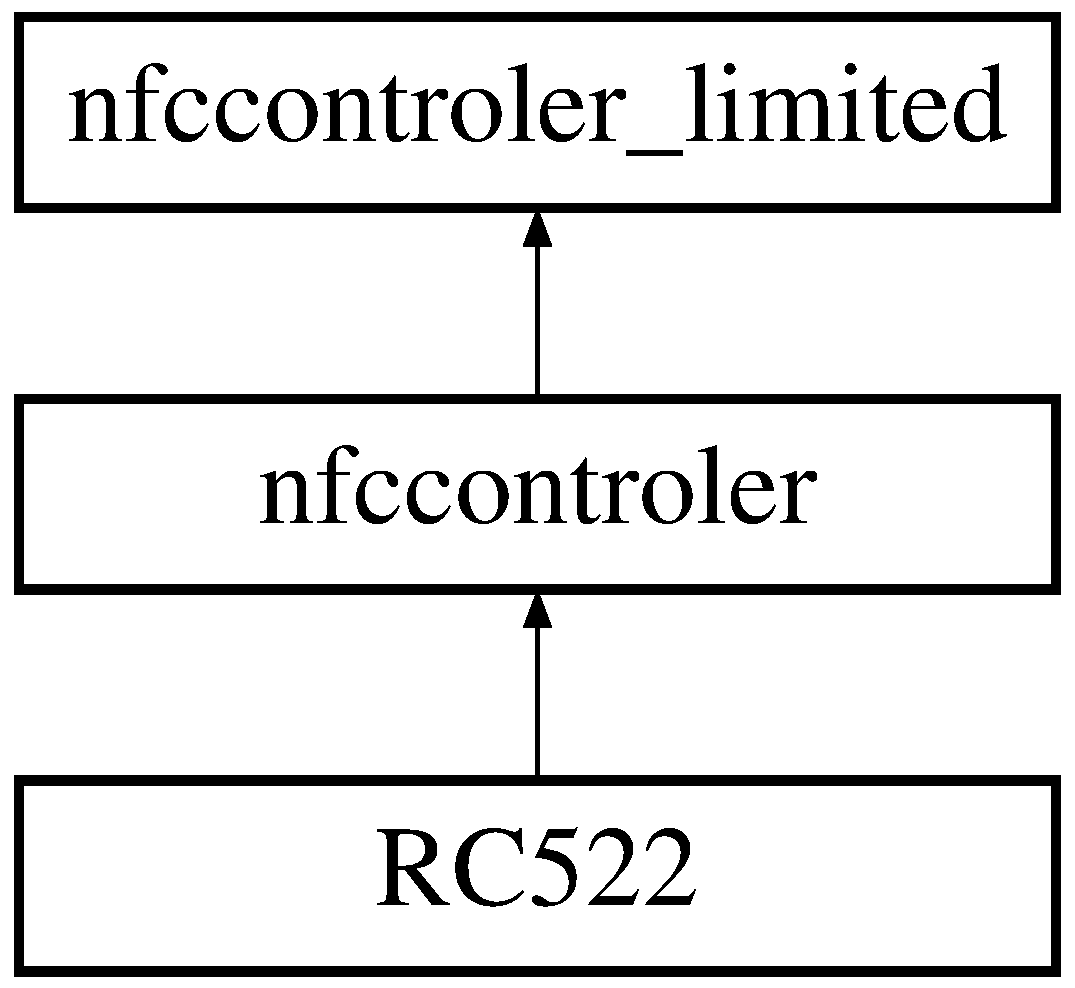
\includegraphics[height=3.000000cm]{classnfccontroler}
\end{center}
\end{figure}
\subsection*{Public Member Functions}
\begin{DoxyCompactItemize}
\item 
virtual byte \hyperlink{classnfccontroler_aaf3c333dece31c91679bb60a58bf1ef9}{read\+Register} (byte register\+Address)=0
\item 
virtual void \hyperlink{classnfccontroler_a0ea9c75e4dbe9dbeb81b49cac5e382db}{write\+Register} (byte register\+Address, byte value)=0
\item 
virtual void \hyperlink{classnfccontroler_af35dd99e72c2321c50dec98529e04a83}{set\+Register\+Mask} (byte register\+Address, byte value)=0
\item 
virtual void \hyperlink{classnfccontroler_a02cfe73ff95bd107f2020ada91ac7af4}{clear\+Register\+Mask} (byte register\+Address, byte value)=0
\item 
virtual byte \hyperlink{classnfccontroler_a99c9451d564a62c525925f8ca79a9d1e}{get\+Antenna\+Gain} (void)=0
\item 
virtual void \hyperlink{classnfccontroler_ae76958998275b8e4acc04c1fe61998e5}{set\+Antenna\+Gain} (byte value)=0
\item 
virtual void \hyperlink{classnfccontroler_a161af319560127b028504add241a8bc6}{antenna\+On} (void)=0
\item 
virtual void \hyperlink{classnfccontroler_a0d8180637c367d223d437a506a641bae}{antenna\+Off} (void)=0
\item 
virtual byte \hyperlink{classnfccontroler_afcab6129cc6c97452f998c46e8088d01}{read\+F\+I\+FO} (void)=0
\item 
virtual int \hyperlink{classnfccontroler_ac1b18db7bd72cf1a2d6cd995ee3919cb}{read\+F\+I\+FO} (byte $\ast$output)=0
\item 
virtual bool \hyperlink{classnfccontroler_aef681b8f4a4a7d982c30ee2d9e8124da}{write\+F\+I\+FO} (const byte value)=0
\item 
virtual bool \hyperlink{classnfccontroler_a5e9de8b00b7bea62fe4f422a898018a9}{write\+F\+I\+FO} (const int byte\+\_\+amount, const byte $\ast$data)=0
\item 
virtual void \hyperlink{classnfccontroler_adf8ddf5ba68a3d6689f5cdc15e294151}{self\+Test} (void)=0
\item 
virtual void \hyperlink{classnfccontroler_a4f5a22e5f25f56abe26ed0034a296135}{init\+Chip} (void)=0
\item 
virtual bool \hyperlink{classnfccontroler_a742e67e43b865074c4f23fb6c133cdd7}{communicate\+N\+FC} (const byte $\ast$data\+\_\+in, const int data\+\_\+in\+\_\+lenght, byte command, byte $\ast$data\+\_\+out, int $\ast$data\+\_\+out\+\_\+lenght, bool crc=false, bool Bitwraping=false)=0
\item 
virtual int \hyperlink{classnfccontroler_a0a04b877e9de8677b5bfe9e28424cbca}{calculate\+C\+RC} (const byte $\ast$data, const int length, byte $\ast$result)=0
\end{DoxyCompactItemize}


\subsection{Detailed Description}
nfccontroler abstraction layer for functions on the microcontroller side of the library.

W\+A\+R\+N\+I\+NG the use of most functions in this class requires I\+N\+T\+I\+M\+A\+TE K\+N\+O\+W\+L\+E\+D\+GE of the inner workings of the microcontroller and its registers. Do N\+OT make use of these functions unless you confidently know what you are doing. The functions in question will be marked with the warning I\+N\+T\+I\+M\+A\+TE K\+N\+O\+W\+L\+E\+D\+GE R\+E\+Q\+U\+I\+R\+ED.

This class contains the nfccontroler abstraction for the reading and writing of microcontroller registers. The setting and clearing of specific bits inside a register. The core functionality of communication used by the microcontroller. And convenience functions for controlling the antenna of the microcontroller. 

\subsection{Member Function Documentation}
\index{nfccontroler@{nfccontroler}!antenna\+Off@{antenna\+Off}}
\index{antenna\+Off@{antenna\+Off}!nfccontroler@{nfccontroler}}
\subsubsection[{\texorpdfstring{antenna\+Off(void)=0}{antennaOff(void)=0}}]{\setlength{\rightskip}{0pt plus 5cm}virtual void nfccontroler\+::antenna\+Off (
\begin{DoxyParamCaption}
\item[{void}]{}
\end{DoxyParamCaption}
)\hspace{0.3cm}{\ttfamily [pure virtual]}}\hypertarget{classnfccontroler_a0d8180637c367d223d437a506a641bae}{}\label{classnfccontroler_a0d8180637c367d223d437a506a641bae}
Function for turning the microcontrollers antena off

Turns the antenna off. 

Implemented in \hyperlink{class_r_c522_a21cce592f19fdbdc440bfec6045eb5ac}{R\+C522}.

\index{nfccontroler@{nfccontroler}!antenna\+On@{antenna\+On}}
\index{antenna\+On@{antenna\+On}!nfccontroler@{nfccontroler}}
\subsubsection[{\texorpdfstring{antenna\+On(void)=0}{antennaOn(void)=0}}]{\setlength{\rightskip}{0pt plus 5cm}virtual void nfccontroler\+::antenna\+On (
\begin{DoxyParamCaption}
\item[{void}]{}
\end{DoxyParamCaption}
)\hspace{0.3cm}{\ttfamily [pure virtual]}}\hypertarget{classnfccontroler_a161af319560127b028504add241a8bc6}{}\label{classnfccontroler_a161af319560127b028504add241a8bc6}
Function for turning the mircocontrollers antenna on.

Turns the antenna on. 

Implemented in \hyperlink{class_r_c522_ae4dbd838876dbd901d811af06e72a448}{R\+C522}.

\index{nfccontroler@{nfccontroler}!calculate\+C\+RC@{calculate\+C\+RC}}
\index{calculate\+C\+RC@{calculate\+C\+RC}!nfccontroler@{nfccontroler}}
\subsubsection[{\texorpdfstring{calculate\+C\+R\+C(const byte $\ast$data, const int length, byte $\ast$result)=0}{calculateCRC(const byte *data, const int length, byte *result)=0}}]{\setlength{\rightskip}{0pt plus 5cm}virtual int nfccontroler\+::calculate\+C\+RC (
\begin{DoxyParamCaption}
\item[{const byte $\ast$}]{data, }
\item[{const int}]{length, }
\item[{byte $\ast$}]{result}
\end{DoxyParamCaption}
)\hspace{0.3cm}{\ttfamily [pure virtual]}}\hypertarget{classnfccontroler_a0a04b877e9de8677b5bfe9e28424cbca}{}\label{classnfccontroler_a0a04b877e9de8677b5bfe9e28424cbca}
Function that calculates the C\+RC for the given data.

W\+A\+R\+N\+I\+NG I\+N\+T\+I\+M\+A\+TE K\+N\+O\+W\+L\+E\+D\+GE R\+E\+Q\+U\+I\+R\+ED

This function takes data in array form into the parameter \textquotesingle{}data\textquotesingle{} Together with the integer \textquotesingle{}length\textquotesingle{} which provides the amount of data it calculates the result and inserts it into the parameter \textquotesingle{}result\textquotesingle{} in array format. this function returns 0 on successfull C\+RC calculation. Otherwise it returns 1; 

Implemented in \hyperlink{class_r_c522_a97d66d97883cf728889098e4a2522f27}{R\+C522}.

\index{nfccontroler@{nfccontroler}!clear\+Register\+Mask@{clear\+Register\+Mask}}
\index{clear\+Register\+Mask@{clear\+Register\+Mask}!nfccontroler@{nfccontroler}}
\subsubsection[{\texorpdfstring{clear\+Register\+Mask(byte register\+Address, byte value)=0}{clearRegisterMask(byte registerAddress, byte value)=0}}]{\setlength{\rightskip}{0pt plus 5cm}virtual void nfccontroler\+::clear\+Register\+Mask (
\begin{DoxyParamCaption}
\item[{byte}]{register\+Address, }
\item[{byte}]{value}
\end{DoxyParamCaption}
)\hspace{0.3cm}{\ttfamily [pure virtual]}}\hypertarget{classnfccontroler_a02cfe73ff95bd107f2020ada91ac7af4}{}\label{classnfccontroler_a02cfe73ff95bd107f2020ada91ac7af4}
Function for altering the settings of a register without overwriting all the bits stored in a register.

W\+A\+R\+N\+I\+NG I\+N\+T\+I\+M\+A\+TE K\+N\+O\+W\+L\+E\+D\+GE R\+E\+Q\+U\+I\+R\+ED

This function resets the given bits in the bite provided. It does this W\+I\+T\+H\+O\+UT altering the other bits in the register. This means that al Z\+E\+R\+O\+ES in the byte will be ignored. The \textquotesingle{}byte register\+Address\textquotesingle{} parameter is used to select the address of the register. The \textquotesingle{}byte value\textquotesingle{} parameter is used to provide the bits to be changed in the register. 

Implemented in \hyperlink{class_r_c522_ac8dda7d6495cd0e79815ba771012b1b4}{R\+C522}.

\index{nfccontroler@{nfccontroler}!communicate\+N\+FC@{communicate\+N\+FC}}
\index{communicate\+N\+FC@{communicate\+N\+FC}!nfccontroler@{nfccontroler}}
\subsubsection[{\texorpdfstring{communicate\+N\+F\+C(const byte $\ast$data\+\_\+in, const int data\+\_\+in\+\_\+lenght, byte command, byte $\ast$data\+\_\+out, int $\ast$data\+\_\+out\+\_\+lenght, bool crc=false, bool Bitwraping=false)=0}{communicateNFC(const byte *data_in, const int data_in_lenght, byte command, byte *data_out, int *data_out_lenght, bool crc=false, bool Bitwraping=false)=0}}]{\setlength{\rightskip}{0pt plus 5cm}virtual bool nfccontroler\+::communicate\+N\+FC (
\begin{DoxyParamCaption}
\item[{const byte $\ast$}]{data\+\_\+in, }
\item[{const int}]{data\+\_\+in\+\_\+lenght, }
\item[{byte}]{command, }
\item[{byte $\ast$}]{data\+\_\+out, }
\item[{int $\ast$}]{data\+\_\+out\+\_\+lenght, }
\item[{bool}]{crc = {\ttfamily false}, }
\item[{bool}]{Bitwraping = {\ttfamily false}}
\end{DoxyParamCaption}
)\hspace{0.3cm}{\ttfamily [pure virtual]}}\hypertarget{classnfccontroler_a742e67e43b865074c4f23fb6c133cdd7}{}\label{classnfccontroler_a742e67e43b865074c4f23fb6c133cdd7}
A function that provides the implementation of sending and receiving data.

W\+A\+R\+N\+I\+NG I\+N\+T\+I\+M\+A\+TE K\+N\+O\+W\+L\+E\+D\+GE R\+E\+Q\+U\+I\+R\+ED

This function provides the core functionality for sending and receiving data. The parameter \textquotesingle{}data\+\_\+in\textquotesingle{} provides the data that is to be sent in array format. In combination with the \textquotesingle{}data\+\_\+in\+\_\+lenght\textquotesingle{} parameter to inform the function the amount of data to be sent. It is important to keep in mind the size of the buffer that transmits the data in order to prevent this from overflowing. When data is received the data itself is inserted into the \textquotesingle{}data\+\_\+out\textquotesingle{} parameter in array form. The amount of bytes received is inserted into the \textquotesingle{}data\+\_\+out\+\_\+lenght\textquotesingle{} parameter.

The Boolean parameter \textquotesingle{}crc\textquotesingle{} tells the function to or not to calculate the C\+RC for the data and add it to the to be sent data. Keep in mind that the C\+RC result itself takes up some space in the buffer.

The Boolean parameter \textquotesingle{}Bitwraping\textquotesingle{} tells the function to or not to use a specified bit-\/frame for sending the data. An example of this is that the \textquotesingle{}M\+I\+F\+A\+RE Classic\textquotesingle{} standard of cards only responds to initial contact when the request command is sent in a seven-\/bit frame.

F\+I\+N\+AL W\+A\+R\+N\+I\+NG this is a complicated function that requires knowledge of both the microcontroller and the card protocol being used. It is recommended that the user first reads the appropriate documentation of both the microcontroller and the protocol in use respectively. U\+SE W\+I\+TH C\+A\+U\+T\+I\+ON 

Implemented in \hyperlink{class_r_c522_aa8ec37f7914b3aa1e3866dda7e08063f}{R\+C522}.

\index{nfccontroler@{nfccontroler}!get\+Antenna\+Gain@{get\+Antenna\+Gain}}
\index{get\+Antenna\+Gain@{get\+Antenna\+Gain}!nfccontroler@{nfccontroler}}
\subsubsection[{\texorpdfstring{get\+Antenna\+Gain(void)=0}{getAntennaGain(void)=0}}]{\setlength{\rightskip}{0pt plus 5cm}virtual byte nfccontroler\+::get\+Antenna\+Gain (
\begin{DoxyParamCaption}
\item[{void}]{}
\end{DoxyParamCaption}
)\hspace{0.3cm}{\ttfamily [pure virtual]}}\hypertarget{classnfccontroler_a99c9451d564a62c525925f8ca79a9d1e}{}\label{classnfccontroler_a99c9451d564a62c525925f8ca79a9d1e}
Function for reading the antennas current Gain setting.

This function returns a byte value that represents the current gain setting of the microcontrollers antenna. The meaning of this byte usually represented in the microcontrollers appropriate documentation. Using this function requires some knowledge of the microcontroller in question, caution is advised. 

Implemented in \hyperlink{class_r_c522_a08a908f30b995446c40b0ba89cf7a40c}{R\+C522}.

\index{nfccontroler@{nfccontroler}!init\+Chip@{init\+Chip}}
\index{init\+Chip@{init\+Chip}!nfccontroler@{nfccontroler}}
\subsubsection[{\texorpdfstring{init\+Chip(void)=0}{initChip(void)=0}}]{\setlength{\rightskip}{0pt plus 5cm}virtual void nfccontroler\+::init\+Chip (
\begin{DoxyParamCaption}
\item[{void}]{}
\end{DoxyParamCaption}
)\hspace{0.3cm}{\ttfamily [pure virtual]}}\hypertarget{classnfccontroler_a4f5a22e5f25f56abe26ed0034a296135}{}\label{classnfccontroler_a4f5a22e5f25f56abe26ed0034a296135}
A Function that readies the microcontroller for sending and receiving data.

This function initializes the basic functions of the chip and configures the needed registers to start sending and receiving data. It also performs a soft reset to make sure the initialization always starts off with the same configuration. The function also turns the antenna on. 

Implemented in \hyperlink{class_r_c522_a87733717cd499f3d51ad9034f78cda9d}{R\+C522}.

\index{nfccontroler@{nfccontroler}!read\+F\+I\+FO@{read\+F\+I\+FO}}
\index{read\+F\+I\+FO@{read\+F\+I\+FO}!nfccontroler@{nfccontroler}}
\subsubsection[{\texorpdfstring{read\+F\+I\+F\+O(void)=0}{readFIFO(void)=0}}]{\setlength{\rightskip}{0pt plus 5cm}virtual byte nfccontroler\+::read\+F\+I\+FO (
\begin{DoxyParamCaption}
\item[{void}]{}
\end{DoxyParamCaption}
)\hspace{0.3cm}{\ttfamily [pure virtual]}}\hypertarget{classnfccontroler_afcab6129cc6c97452f998c46e8088d01}{}\label{classnfccontroler_afcab6129cc6c97452f998c46e8088d01}
A function that returns a single byte from the F\+I\+F\+O-\/buffer.

W\+A\+R\+N\+I\+NG I\+N\+T\+I\+M\+A\+TE K\+N\+O\+W\+L\+E\+D\+GE R\+E\+Q\+U\+I\+R\+ED

This function reads a single byte from the F\+I\+F\+O-\/buffer and returns this. W\+A\+R\+N\+I\+NG make sure you know if the F\+I\+F\+O-\/buffer of your microcontroller preserves its data when read. An example of this is the F\+I\+F\+O-\/buffer from the \hyperlink{class_r_c522}{R\+C522} which deletes the byte read from the buffer afterwards. To prevent data loss make sure the byte returned is stored somewhere if this situation occurs. 

Implemented in \hyperlink{class_r_c522_a78c18a8805798cda24ed7c35af43f6c3}{R\+C522}.

\index{nfccontroler@{nfccontroler}!read\+F\+I\+FO@{read\+F\+I\+FO}}
\index{read\+F\+I\+FO@{read\+F\+I\+FO}!nfccontroler@{nfccontroler}}
\subsubsection[{\texorpdfstring{read\+F\+I\+F\+O(byte $\ast$output)=0}{readFIFO(byte *output)=0}}]{\setlength{\rightskip}{0pt plus 5cm}virtual int nfccontroler\+::read\+F\+I\+FO (
\begin{DoxyParamCaption}
\item[{byte $\ast$}]{output}
\end{DoxyParamCaption}
)\hspace{0.3cm}{\ttfamily [pure virtual]}}\hypertarget{classnfccontroler_ac1b18db7bd72cf1a2d6cd995ee3919cb}{}\label{classnfccontroler_ac1b18db7bd72cf1a2d6cd995ee3919cb}
Function for reading data currently stored in the F\+I\+F\+O-\/buffer.

W\+A\+R\+N\+I\+NG I\+N\+T\+I\+M\+A\+TE K\+N\+O\+W\+L\+E\+D\+GE R\+E\+Q\+U\+I\+R\+ED

This function reads all data currently stored in the F\+I\+F\+O-\/buffer. It inserts this data into the \textquotesingle{}output\textquotesingle{} parameter in array from. The integer value returned is the amount of bytes about to be read from the buffer W\+A\+R\+N\+I\+NG make sure you know if the F\+I\+F\+O-\/buffer of your microcontroller preserves its data when read. An example of this is the F\+I\+F\+O-\/buffer from the \hyperlink{class_r_c522}{R\+C522} which deletes the byte read from the buffer afterwards. To prevent data loss make sure the data is stored somewhere if this situation occurs. It is important to know the maximum amount of data the buffer can hold so you can provide appropriate storage. 

Implemented in \hyperlink{class_r_c522_a2e5ac8769707047e4064200d1829927c}{R\+C522}.

\index{nfccontroler@{nfccontroler}!read\+Register@{read\+Register}}
\index{read\+Register@{read\+Register}!nfccontroler@{nfccontroler}}
\subsubsection[{\texorpdfstring{read\+Register(byte register\+Address)=0}{readRegister(byte registerAddress)=0}}]{\setlength{\rightskip}{0pt plus 5cm}virtual byte nfccontroler\+::read\+Register (
\begin{DoxyParamCaption}
\item[{byte}]{register\+Address}
\end{DoxyParamCaption}
)\hspace{0.3cm}{\ttfamily [pure virtual]}}\hypertarget{classnfccontroler_aaf3c333dece31c91679bb60a58bf1ef9}{}\label{classnfccontroler_aaf3c333dece31c91679bb60a58bf1ef9}
Function for reading the current settings of a register.

W\+A\+R\+N\+I\+NG I\+N\+T\+I\+M\+A\+TE K\+N\+O\+W\+L\+E\+D\+GE R\+E\+Q\+U\+I\+R\+ED

This function returns the current bits set in a register in the form of a single byte. The parameter \textquotesingle{}byte register\+Address\textquotesingle{} is used to supply the address of the register.

W\+A\+R\+N\+I\+NG make sure you know if the register you are reading from preserves its data when read. An example of this is the F\+I\+F\+O-\/buffer from the \hyperlink{class_r_c522}{R\+C522} which deletes the byte read from the buffer afterwards. To prevent data loss make sure the byte returned is stored somewhere if this situation occurs. 

Implemented in \hyperlink{class_r_c522_a5de4e5d16b9d54c859f6db3de68c8147}{R\+C522}.

\index{nfccontroler@{nfccontroler}!self\+Test@{self\+Test}}
\index{self\+Test@{self\+Test}!nfccontroler@{nfccontroler}}
\subsubsection[{\texorpdfstring{self\+Test(void)=0}{selfTest(void)=0}}]{\setlength{\rightskip}{0pt plus 5cm}virtual void nfccontroler\+::self\+Test (
\begin{DoxyParamCaption}
\item[{void}]{}
\end{DoxyParamCaption}
)\hspace{0.3cm}{\ttfamily [pure virtual]}}\hypertarget{classnfccontroler_adf8ddf5ba68a3d6689f5cdc15e294151}{}\label{classnfccontroler_adf8ddf5ba68a3d6689f5cdc15e294151}
A Function that runs the self test function of the microcontroller in question.

The results of the self test are printed to the terminal and can be compared to the expected results usually defined in the microcontroller’s documentation. 

Implemented in \hyperlink{class_r_c522_ad21aeb49627a3da99d214798886267b9}{R\+C522}.

\index{nfccontroler@{nfccontroler}!set\+Antenna\+Gain@{set\+Antenna\+Gain}}
\index{set\+Antenna\+Gain@{set\+Antenna\+Gain}!nfccontroler@{nfccontroler}}
\subsubsection[{\texorpdfstring{set\+Antenna\+Gain(byte value)=0}{setAntennaGain(byte value)=0}}]{\setlength{\rightskip}{0pt plus 5cm}virtual void nfccontroler\+::set\+Antenna\+Gain (
\begin{DoxyParamCaption}
\item[{byte}]{value}
\end{DoxyParamCaption}
)\hspace{0.3cm}{\ttfamily [pure virtual]}}\hypertarget{classnfccontroler_ae76958998275b8e4acc04c1fe61998e5}{}\label{classnfccontroler_ae76958998275b8e4acc04c1fe61998e5}
Function for setting the antennas gain.

This function sets the gain level of the antenna by sending a byte to the antennas register. The meaning of the bits contained in the byte is usually represented in the microcontrollers appropriate documentation. Using this function requires some knowledge of the microcontroller in question, caution is advised. 

Implemented in \hyperlink{class_r_c522_aa5a6532f6ef2de5ca9236567ff88d346}{R\+C522}.

\index{nfccontroler@{nfccontroler}!set\+Register\+Mask@{set\+Register\+Mask}}
\index{set\+Register\+Mask@{set\+Register\+Mask}!nfccontroler@{nfccontroler}}
\subsubsection[{\texorpdfstring{set\+Register\+Mask(byte register\+Address, byte value)=0}{setRegisterMask(byte registerAddress, byte value)=0}}]{\setlength{\rightskip}{0pt plus 5cm}virtual void nfccontroler\+::set\+Register\+Mask (
\begin{DoxyParamCaption}
\item[{byte}]{register\+Address, }
\item[{byte}]{value}
\end{DoxyParamCaption}
)\hspace{0.3cm}{\ttfamily [pure virtual]}}\hypertarget{classnfccontroler_af35dd99e72c2321c50dec98529e04a83}{}\label{classnfccontroler_af35dd99e72c2321c50dec98529e04a83}
Function for altering the settings of a register without overwriting all the bits stored in a register.

W\+A\+R\+N\+I\+NG I\+N\+T\+I\+M\+A\+TE K\+N\+O\+W\+L\+E\+D\+GE R\+E\+Q\+U\+I\+R\+ED

This function sets the given bits in the bite provided. It does this W\+I\+T\+H\+O\+UT altering the other bits in the register. This means that al Z\+E\+R\+O\+ES in the byte will be ignored. The \textquotesingle{}byte register\+Address\textquotesingle{} parameter is used to select the address of the register. The \textquotesingle{}byte value\textquotesingle{} parameter is used to provide the bits to be changed in the register. 

Implemented in \hyperlink{class_r_c522_a14cc49cb3afd67164ebceffdb38dd605}{R\+C522}.

\index{nfccontroler@{nfccontroler}!write\+F\+I\+FO@{write\+F\+I\+FO}}
\index{write\+F\+I\+FO@{write\+F\+I\+FO}!nfccontroler@{nfccontroler}}
\subsubsection[{\texorpdfstring{write\+F\+I\+F\+O(const byte value)=0}{writeFIFO(const byte value)=0}}]{\setlength{\rightskip}{0pt plus 5cm}virtual bool nfccontroler\+::write\+F\+I\+FO (
\begin{DoxyParamCaption}
\item[{const byte}]{value}
\end{DoxyParamCaption}
)\hspace{0.3cm}{\ttfamily [pure virtual]}}\hypertarget{classnfccontroler_aef681b8f4a4a7d982c30ee2d9e8124da}{}\label{classnfccontroler_aef681b8f4a4a7d982c30ee2d9e8124da}
A function that writes a single byte to the F\+I\+F\+O-\/buffer.

W\+A\+R\+N\+I\+NG I\+N\+T\+I\+M\+A\+TE K\+N\+O\+W\+L\+E\+D\+GE R\+E\+Q\+U\+I\+R\+ED

This function writes a single byte to the F\+I\+F\+O-\/buffer. It will return false if the F\+I\+F\+O-\/buffer is full. The parameter \textquotesingle{}value\textquotesingle{} is used to provide the byte of data that needs to be written to the F\+I\+F\+O-\/buffer. It is recommended that you know the size of your microcontroller’s F\+I\+F\+O-\/buffer to prevent data loss. 

Implemented in \hyperlink{class_r_c522_a3923806b946c8e35465faca39095fe05}{R\+C522}.

\index{nfccontroler@{nfccontroler}!write\+F\+I\+FO@{write\+F\+I\+FO}}
\index{write\+F\+I\+FO@{write\+F\+I\+FO}!nfccontroler@{nfccontroler}}
\subsubsection[{\texorpdfstring{write\+F\+I\+F\+O(const int byte\+\_\+amount, const byte $\ast$data)=0}{writeFIFO(const int byte_amount, const byte *data)=0}}]{\setlength{\rightskip}{0pt plus 5cm}virtual bool nfccontroler\+::write\+F\+I\+FO (
\begin{DoxyParamCaption}
\item[{const int}]{byte\+\_\+amount, }
\item[{const byte $\ast$}]{data}
\end{DoxyParamCaption}
)\hspace{0.3cm}{\ttfamily [pure virtual]}}\hypertarget{classnfccontroler_a5e9de8b00b7bea62fe4f422a898018a9}{}\label{classnfccontroler_a5e9de8b00b7bea62fe4f422a898018a9}
A function that writes data to the F\+I\+F\+O-\/buffer.

W\+A\+R\+N\+I\+NG I\+N\+T\+I\+M\+A\+TE K\+N\+O\+W\+L\+E\+D\+GE R\+E\+Q\+U\+I\+R\+ED

This function writes the data provided byte to the F\+I\+F\+O-\/buffer. It will return false if the F\+I\+F\+O-\/buffer is full or if you provide so much data that the buffer will overflow. The \textquotesingle{}byte\+\_\+amount\textquotesingle{} parameter is used to provide the amount of data about to be sent to the F\+I\+F\+O-\/buffer. the \textquotesingle{}data\textquotesingle{} parameter is used to provide the actual data to be written in array form. It is recommended that you know the size of your microcontroller’s F\+I\+F\+O-\/buffer to prevent data loss. 

Implemented in \hyperlink{class_r_c522_ac72080585e07afd1d51fbb4dbc6a8e58}{R\+C522}.

\index{nfccontroler@{nfccontroler}!write\+Register@{write\+Register}}
\index{write\+Register@{write\+Register}!nfccontroler@{nfccontroler}}
\subsubsection[{\texorpdfstring{write\+Register(byte register\+Address, byte value)=0}{writeRegister(byte registerAddress, byte value)=0}}]{\setlength{\rightskip}{0pt plus 5cm}virtual void nfccontroler\+::write\+Register (
\begin{DoxyParamCaption}
\item[{byte}]{register\+Address, }
\item[{byte}]{value}
\end{DoxyParamCaption}
)\hspace{0.3cm}{\ttfamily [pure virtual]}}\hypertarget{classnfccontroler_a0ea9c75e4dbe9dbeb81b49cac5e382db}{}\label{classnfccontroler_a0ea9c75e4dbe9dbeb81b49cac5e382db}
Function for writing a single byte to a register.

W\+A\+R\+N\+I\+NG I\+N\+T\+I\+M\+A\+TE K\+N\+O\+W\+L\+E\+D\+GE R\+E\+Q\+U\+I\+R\+ED

This function writes a single byte of data to the selected register. The \textquotesingle{}byte register\+Address\textquotesingle{} parameter is used to select the address of the register. The \textquotesingle{}byte value\textquotesingle{} parameter is used to provide the byte to be written.

W\+A\+R\+N\+I\+NG this function sends the whole byte of data to be written to the register. It can potentially overwrite previously set settings of that register. 

Implemented in \hyperlink{class_r_c522_a8860f482253b39808658bf5cdbbe342d}{R\+C522}.



The documentation for this class was generated from the following file\+:\begin{DoxyCompactItemize}
\item 
\hyperlink{nfccontroler_8hpp}{nfccontroler.\+hpp}\end{DoxyCompactItemize}

\hypertarget{classnfccontroler__limited}{}\section{nfccontroler\+\_\+limited Class Reference}
\label{classnfccontroler__limited}\index{nfccontroler\+\_\+limited@{nfccontroler\+\_\+limited}}


{\ttfamily \#include $<$nfccontroler\+\_\+limited.\+hpp$>$}

Inheritance diagram for nfccontroler\+\_\+limited\+:\begin{figure}[H]
\begin{center}
\leavevmode
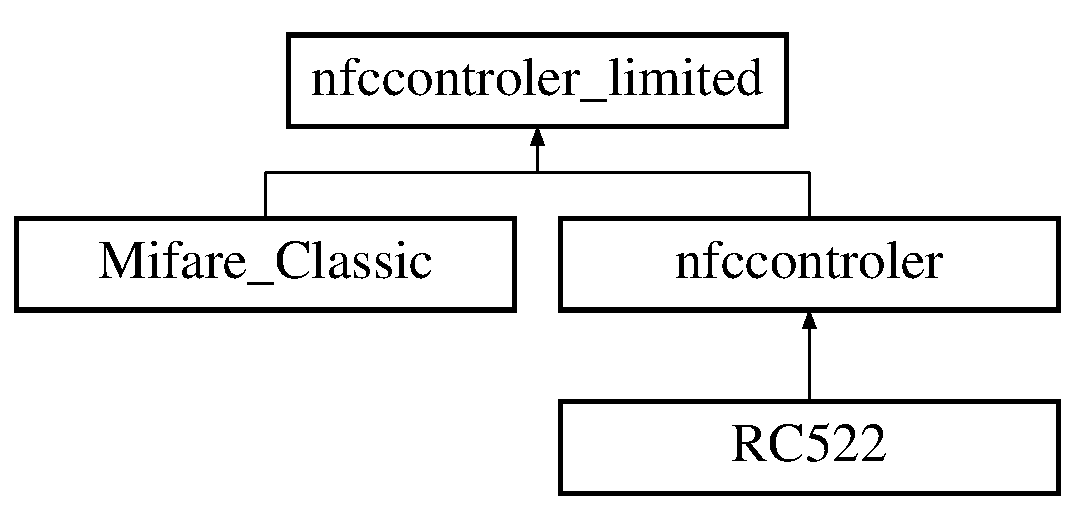
\includegraphics[height=3.000000cm]{classnfccontroler__limited}
\end{center}
\end{figure}
\subsection*{Public Member Functions}
\begin{DoxyCompactItemize}
\item 
virtual void \hyperlink{classnfccontroler__limited_a97f279888626df09059338d149a3dcf1}{check\+Erro\+And\+Irq} (byte $\ast$result)=0
\item 
virtual bool \hyperlink{classnfccontroler__limited_a35a7cc1d586511b6a35294bc234530e0}{trancieve\+Data} (const byte $\ast$data\+\_\+in, const int data\+\_\+in\+\_\+lenght, byte $\ast$data\+\_\+out, int $\ast$data\+\_\+out\+\_\+lenght, bool crc=false, bool Bitwraping=false)=0
\item 
virtual bool \hyperlink{classnfccontroler__limited_ae1e689d34ba8bcd933c696b3f852dad6}{is\+Card} (byte $\ast$cardtype)=0
\item 
virtual bool \hyperlink{classnfccontroler__limited_a195f3de8d1529e00998f60ddf8058f6b}{select\+Card} (byte $\ast$Cardserial)=0
\item 
virtual bool \hyperlink{classnfccontroler__limited_a4eec4cf702e4c0062c33657e81a2069f}{authenticate\+Sector} (byte typekey, byte $\ast$block\+\_\+address, byte $\ast$key, byte $\ast$Cardserial)=0
\item 
virtual bool \hyperlink{classnfccontroler__limited_a5a8f607de57023a90962f6ac4fa2b5f1}{read\+Block} (byte block\+\_\+address, byte $\ast$data\+\_\+out)=0
\item 
virtual bool \hyperlink{classnfccontroler__limited_a70d6de379a501af2272da775c5d27c9e}{read\+Sector} (const int sectorsize, byte($\ast$sector\+\_\+out)\mbox{[}16\mbox{]}, byte typekey, byte $\ast$first\+\_\+block\+\_\+in\+\_\+sector, byte $\ast$key, byte $\ast$Cardserial)=0
\item 
virtual bool \hyperlink{classnfccontroler__limited_aeeeb82c8b45881239c7b2d9b4bce9ef5}{write\+Block} (const byte block\+\_\+address, const byte $\ast$data\+\_\+in, const int lenght)=0
\item 
virtual bool \hyperlink{classnfccontroler__limited_ad4d31d46ee21766eaaa0a4f1916cc8d8}{write\+Sector} (const int sectorsize, byte($\ast$sector\+\_\+in)\mbox{[}16\mbox{]}, byte typekey, byte $\ast$first\+\_\+block\+\_\+in\+\_\+sector, byte $\ast$key, byte $\ast$Cardserial)=0
\end{DoxyCompactItemize}


\subsection{Detailed Description}
nfccontroler abstraction layer for functions on the card protocol side of the library.

This class contains the nfccontroler abstraction for the detection, selection, communication and error checking when communicating with an N\+FC card. 

\subsection{Member Function Documentation}
\index{nfccontroler\+\_\+limited@{nfccontroler\+\_\+limited}!authenticate\+Sector@{authenticate\+Sector}}
\index{authenticate\+Sector@{authenticate\+Sector}!nfccontroler\+\_\+limited@{nfccontroler\+\_\+limited}}
\subsubsection[{\texorpdfstring{authenticate\+Sector(byte typekey, byte $\ast$block\+\_\+address, byte $\ast$key, byte $\ast$\+Cardserial)=0}{authenticateSector(byte typekey, byte *block_address, byte *key, byte *Cardserial)=0}}]{\setlength{\rightskip}{0pt plus 5cm}virtual bool nfccontroler\+\_\+limited\+::authenticate\+Sector (
\begin{DoxyParamCaption}
\item[{byte}]{typekey, }
\item[{byte $\ast$}]{block\+\_\+address, }
\item[{byte $\ast$}]{key, }
\item[{byte $\ast$}]{Cardserial}
\end{DoxyParamCaption}
)\hspace{0.3cm}{\ttfamily [pure virtual]}}\hypertarget{classnfccontroler__limited_a4eec4cf702e4c0062c33657e81a2069f}{}\label{classnfccontroler__limited_a4eec4cf702e4c0062c33657e81a2069f}
Function for authenticating access to a sector.

This function grants access to the specified sector of the card. The typekey parameter is used to specify which key is used for authentication. The block\+\_\+address parameter is used to select which sector is authenticated for. The key parameter is used to provide they key in byte array form to the specified sector. Any block in a sector may be targeted for authentication and will grant access to all blocks in that sector. This function returns true after successful authentication. 

Implemented in \hyperlink{class_r_c522_a84000801a44a02cf59601400b809f5a3}{R\+C522}, and \hyperlink{class_mifare___classic_a2e79d1842e44e1600f59fdfba4b22470}{Mifare\+\_\+\+Classic}.

\index{nfccontroler\+\_\+limited@{nfccontroler\+\_\+limited}!check\+Erro\+And\+Irq@{check\+Erro\+And\+Irq}}
\index{check\+Erro\+And\+Irq@{check\+Erro\+And\+Irq}!nfccontroler\+\_\+limited@{nfccontroler\+\_\+limited}}
\subsubsection[{\texorpdfstring{check\+Erro\+And\+Irq(byte $\ast$result)=0}{checkErroAndIrq(byte *result)=0}}]{\setlength{\rightskip}{0pt plus 5cm}virtual void nfccontroler\+\_\+limited\+::check\+Erro\+And\+Irq (
\begin{DoxyParamCaption}
\item[{byte $\ast$}]{result}
\end{DoxyParamCaption}
)\hspace{0.3cm}{\ttfamily [pure virtual]}}\hypertarget{classnfccontroler__limited_a97f279888626df09059338d149a3dcf1}{}\label{classnfccontroler__limited_a97f279888626df09059338d149a3dcf1}
Function checking the error and I\+RQ results after sending or receiving data.

This function inserts the status of the registers in a byte array that is given to the function as a parameter.

The use function requires knowledge of how the chip returns these results. 

Implemented in \hyperlink{class_r_c522_a8797a7dcb6e4a7e3e30bf476ef47e894}{R\+C522}, and \hyperlink{class_mifare___classic_a9377d560c083320ad3b605df464a29e4}{Mifare\+\_\+\+Classic}.

\index{nfccontroler\+\_\+limited@{nfccontroler\+\_\+limited}!is\+Card@{is\+Card}}
\index{is\+Card@{is\+Card}!nfccontroler\+\_\+limited@{nfccontroler\+\_\+limited}}
\subsubsection[{\texorpdfstring{is\+Card(byte $\ast$cardtype)=0}{isCard(byte *cardtype)=0}}]{\setlength{\rightskip}{0pt plus 5cm}virtual bool nfccontroler\+\_\+limited\+::is\+Card (
\begin{DoxyParamCaption}
\item[{byte $\ast$}]{cardtype}
\end{DoxyParamCaption}
)\hspace{0.3cm}{\ttfamily [pure virtual]}}\hypertarget{classnfccontroler__limited_ae1e689d34ba8bcd933c696b3f852dad6}{}\label{classnfccontroler__limited_ae1e689d34ba8bcd933c696b3f852dad6}
Function for detecting if a card is in the EM field.

This function constantly polls for a card in the EM field When a card responds it inserts the response (Sak) in the cardtype byte array. This response can be used to identify the type of card. Before a card responds to this function it will not respond to any other command. It is currently not supported to have multiple cards in the EM field at the same time. Function will return true on successful detection of a card. 

Implemented in \hyperlink{class_r_c522_a6cef2c82c923eeed59bd3cb5e7a42090}{R\+C522}, and \hyperlink{class_mifare___classic_ae02721fc8b9268e93778fdc47d06d162}{Mifare\+\_\+\+Classic}.

\index{nfccontroler\+\_\+limited@{nfccontroler\+\_\+limited}!read\+Block@{read\+Block}}
\index{read\+Block@{read\+Block}!nfccontroler\+\_\+limited@{nfccontroler\+\_\+limited}}
\subsubsection[{\texorpdfstring{read\+Block(byte block\+\_\+address, byte $\ast$data\+\_\+out)=0}{readBlock(byte block_address, byte *data_out)=0}}]{\setlength{\rightskip}{0pt plus 5cm}virtual bool nfccontroler\+\_\+limited\+::read\+Block (
\begin{DoxyParamCaption}
\item[{byte}]{block\+\_\+address, }
\item[{byte $\ast$}]{data\+\_\+out}
\end{DoxyParamCaption}
)\hspace{0.3cm}{\ttfamily [pure virtual]}}\hypertarget{classnfccontroler__limited_a5a8f607de57023a90962f6ac4fa2b5f1}{}\label{classnfccontroler__limited_a5a8f607de57023a90962f6ac4fa2b5f1}
Function for reading a block of data from the card.

This function reads data from a single block of data inside the card. After reading the data it inserts this in the data\+\_\+out array parameter. It is required to authenticate for the sector that the block resides in before attempting to read. Upon successful reading of data this function returns true. 

Implemented in \hyperlink{class_r_c522_a4a9843ee47bd24f6446bb8c327411076}{R\+C522}, and \hyperlink{class_mifare___classic_a6401f278760213b5c53e3c41aa5b0c98}{Mifare\+\_\+\+Classic}.

\index{nfccontroler\+\_\+limited@{nfccontroler\+\_\+limited}!read\+Sector@{read\+Sector}}
\index{read\+Sector@{read\+Sector}!nfccontroler\+\_\+limited@{nfccontroler\+\_\+limited}}
\subsubsection[{\texorpdfstring{read\+Sector(const int sectorsize, byte($\ast$sector\+\_\+out)[16], byte typekey, byte $\ast$first\+\_\+block\+\_\+in\+\_\+sector, byte $\ast$key, byte $\ast$\+Cardserial)=0}{readSector(const int sectorsize, byte(*sector_out)[16], byte typekey, byte *first_block_in_sector, byte *key, byte *Cardserial)=0}}]{\setlength{\rightskip}{0pt plus 5cm}virtual bool nfccontroler\+\_\+limited\+::read\+Sector (
\begin{DoxyParamCaption}
\item[{const int}]{sectorsize, }
\item[{byte($\ast$)}]{sector\+\_\+out\mbox{[}16\mbox{]}, }
\item[{byte}]{typekey, }
\item[{byte $\ast$}]{first\+\_\+block\+\_\+in\+\_\+sector, }
\item[{byte $\ast$}]{key, }
\item[{byte $\ast$}]{Cardserial}
\end{DoxyParamCaption}
)\hspace{0.3cm}{\ttfamily [pure virtual]}}\hypertarget{classnfccontroler__limited_a70d6de379a501af2272da775c5d27c9e}{}\label{classnfccontroler__limited_a70d6de379a501af2272da775c5d27c9e}
Function for reading an entire sector of data from the card.

This function reads an entire sector of data. After reading the data it inserts this in the sector\+\_\+out 2d matrix parameter. Authentication is built in for this function. The typekey parameter is used to specify which key is used for authentication. The first\+\_\+block\+\_\+in\+\_\+sector parameter is used to select which sector is authenticated for. The key parameter is used to provide they key in byte array form to the specified sector. Upon successful reading of the sector this function returns true. 

Implemented in \hyperlink{class_r_c522_a6c6409ef5f4385e9d1efac5b2f9caed0}{R\+C522}, and \hyperlink{class_mifare___classic_a7caca9ec9a0cdc116f8056753ecc438c}{Mifare\+\_\+\+Classic}.

\index{nfccontroler\+\_\+limited@{nfccontroler\+\_\+limited}!select\+Card@{select\+Card}}
\index{select\+Card@{select\+Card}!nfccontroler\+\_\+limited@{nfccontroler\+\_\+limited}}
\subsubsection[{\texorpdfstring{select\+Card(byte $\ast$\+Cardserial)=0}{selectCard(byte *Cardserial)=0}}]{\setlength{\rightskip}{0pt plus 5cm}virtual bool nfccontroler\+\_\+limited\+::select\+Card (
\begin{DoxyParamCaption}
\item[{byte $\ast$}]{Cardserial}
\end{DoxyParamCaption}
)\hspace{0.3cm}{\ttfamily [pure virtual]}}\hypertarget{classnfccontroler__limited_a195f3de8d1529e00998f60ddf8058f6b}{}\label{classnfccontroler__limited_a195f3de8d1529e00998f60ddf8058f6b}
Function for the selection of the card.

This function requests the U\+ID (Unique Identifier) from the card and then uses the U\+ID to select the card. It inserts the U\+ID into the Cardserial array. When a card has been successfully selected its U\+ID can be used to send other data and commands towards the card. This function returns true after the successful selection of a card. 

Implemented in \hyperlink{class_r_c522_a2b41c31a04a41b6098945b0fddcf1476}{R\+C522}, and \hyperlink{class_mifare___classic_aaa549c00df8619bb2f5a96bba093f005}{Mifare\+\_\+\+Classic}.

\index{nfccontroler\+\_\+limited@{nfccontroler\+\_\+limited}!trancieve\+Data@{trancieve\+Data}}
\index{trancieve\+Data@{trancieve\+Data}!nfccontroler\+\_\+limited@{nfccontroler\+\_\+limited}}
\subsubsection[{\texorpdfstring{trancieve\+Data(const byte $\ast$data\+\_\+in, const int data\+\_\+in\+\_\+lenght, byte $\ast$data\+\_\+out, int $\ast$data\+\_\+out\+\_\+lenght, bool crc=false, bool Bitwraping=false)=0}{trancieveData(const byte *data_in, const int data_in_lenght, byte *data_out, int *data_out_lenght, bool crc=false, bool Bitwraping=false)=0}}]{\setlength{\rightskip}{0pt plus 5cm}virtual bool nfccontroler\+\_\+limited\+::trancieve\+Data (
\begin{DoxyParamCaption}
\item[{const byte $\ast$}]{data\+\_\+in, }
\item[{const int}]{data\+\_\+in\+\_\+lenght, }
\item[{byte $\ast$}]{data\+\_\+out, }
\item[{int $\ast$}]{data\+\_\+out\+\_\+lenght, }
\item[{bool}]{crc = {\ttfamily false}, }
\item[{bool}]{Bitwraping = {\ttfamily false}}
\end{DoxyParamCaption}
)\hspace{0.3cm}{\ttfamily [pure virtual]}}\hypertarget{classnfccontroler__limited_a35a7cc1d586511b6a35294bc234530e0}{}\label{classnfccontroler__limited_a35a7cc1d586511b6a35294bc234530e0}
Function for using the simultaneous sending and receiving of data.

This function is used for sending data and commands to the card in the form of bytes. It sends the data stored in a byte array. After sending the data it inserts any received data in the data\+\_\+out array. It will also supply the amount of bytes received unless a nullptr is given to data\+\_\+out\+\_\+lenght. The crc and Bitwraping Booleans are used to trigger the additional functionality of Calculating and adding the crc and the use of a specialised bit frame for certain commands respectively. It is recommended to at least have a basic understanding of the card-\/protocol and microcontroller in use when using this function. 

Implemented in \hyperlink{class_r_c522_a8204221660aea7c393eb49340d29876a}{R\+C522}, and \hyperlink{class_mifare___classic_ac35863ec691f0a118156bea44c4cd7a7}{Mifare\+\_\+\+Classic}.

\index{nfccontroler\+\_\+limited@{nfccontroler\+\_\+limited}!write\+Block@{write\+Block}}
\index{write\+Block@{write\+Block}!nfccontroler\+\_\+limited@{nfccontroler\+\_\+limited}}
\subsubsection[{\texorpdfstring{write\+Block(const byte block\+\_\+address, const byte $\ast$data\+\_\+in, const int lenght)=0}{writeBlock(const byte block_address, const byte *data_in, const int lenght)=0}}]{\setlength{\rightskip}{0pt plus 5cm}virtual bool nfccontroler\+\_\+limited\+::write\+Block (
\begin{DoxyParamCaption}
\item[{const byte}]{block\+\_\+address, }
\item[{const byte $\ast$}]{data\+\_\+in, }
\item[{const int}]{lenght}
\end{DoxyParamCaption}
)\hspace{0.3cm}{\ttfamily [pure virtual]}}\hypertarget{classnfccontroler__limited_aeeeb82c8b45881239c7b2d9b4bce9ef5}{}\label{classnfccontroler__limited_aeeeb82c8b45881239c7b2d9b4bce9ef5}
Function for writing a block of data to the card.

This function writes data to a single block of data inside the card. The parameter data\+\_\+in is used to provide the data to write in byte array form. The data given to the function is appended with zeroes so a full block is always written. It is required to authenticate for the sector that the block resides in before attempting to write. Upon successful writing of data this function returns true. 

Implemented in \hyperlink{class_r_c522_a42c197d61571667a97176f7294b0a8dd}{R\+C522}, and \hyperlink{class_mifare___classic_adb793958d3f2601d336165e383a456f6}{Mifare\+\_\+\+Classic}.

\index{nfccontroler\+\_\+limited@{nfccontroler\+\_\+limited}!write\+Sector@{write\+Sector}}
\index{write\+Sector@{write\+Sector}!nfccontroler\+\_\+limited@{nfccontroler\+\_\+limited}}
\subsubsection[{\texorpdfstring{write\+Sector(const int sectorsize, byte($\ast$sector\+\_\+in)[16], byte typekey, byte $\ast$first\+\_\+block\+\_\+in\+\_\+sector, byte $\ast$key, byte $\ast$\+Cardserial)=0}{writeSector(const int sectorsize, byte(*sector_in)[16], byte typekey, byte *first_block_in_sector, byte *key, byte *Cardserial)=0}}]{\setlength{\rightskip}{0pt plus 5cm}virtual bool nfccontroler\+\_\+limited\+::write\+Sector (
\begin{DoxyParamCaption}
\item[{const int}]{sectorsize, }
\item[{byte($\ast$)}]{sector\+\_\+in\mbox{[}16\mbox{]}, }
\item[{byte}]{typekey, }
\item[{byte $\ast$}]{first\+\_\+block\+\_\+in\+\_\+sector, }
\item[{byte $\ast$}]{key, }
\item[{byte $\ast$}]{Cardserial}
\end{DoxyParamCaption}
)\hspace{0.3cm}{\ttfamily [pure virtual]}}\hypertarget{classnfccontroler__limited_ad4d31d46ee21766eaaa0a4f1916cc8d8}{}\label{classnfccontroler__limited_ad4d31d46ee21766eaaa0a4f1916cc8d8}
Function for writing an entire sector of data to the card.

This function writes an entire sector of data. The sector\+\_\+in parameter is used to provide the data to be written in 2d matrix form. Authentication is built in for this function. The typekey parameter is used to specify which key is used for authentication. The first\+\_\+block\+\_\+in\+\_\+sector parameter is used to select which sector is authenticated for. The key parameter is used to provide they key in byte array form to the specified sector. Upon successful writing of the sector this function returns true. 

Implemented in \hyperlink{class_r_c522_a11e060e686331017873edd877c3255cd}{R\+C522}, and \hyperlink{class_mifare___classic_a127803e07c148fe8d447a00e28be4a90}{Mifare\+\_\+\+Classic}.



The documentation for this class was generated from the following file\+:\begin{DoxyCompactItemize}
\item 
\hyperlink{nfccontroler__limited_8hpp}{nfccontroler\+\_\+limited.\+hpp}\end{DoxyCompactItemize}

\hypertarget{class_r_c522}{}\section{R\+C522 Class Reference}
\label{class_r_c522}\index{R\+C522@{R\+C522}}


{\ttfamily \#include $<$R\+C522.\+hpp$>$}

Inheritance diagram for R\+C522\+:\begin{figure}[H]
\begin{center}
\leavevmode
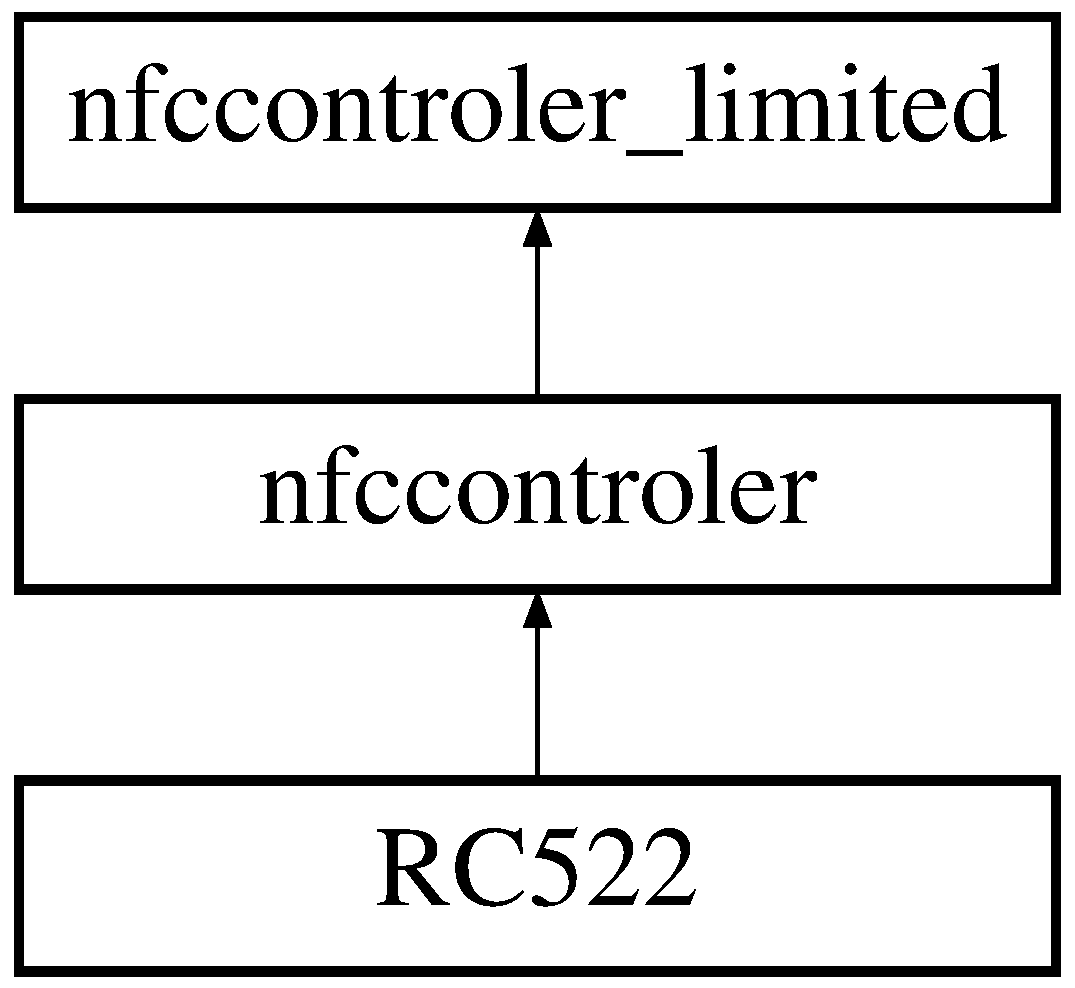
\includegraphics[height=3.000000cm]{class_r_c522}
\end{center}
\end{figure}
\subsection*{Public Types}
\begin{DoxyCompactItemize}
\item 
enum \hyperlink{class_r_c522_a3dcadf9d9544de3a436a34018dea676b}{Keytype} \{ \hyperlink{class_r_c522_a3dcadf9d9544de3a436a34018dea676ba1e7b8f8d328f24fb6773e9656f1ed5be}{Keytype\+::\+AuthwithA} = 0x60, 
\hyperlink{class_r_c522_a3dcadf9d9544de3a436a34018dea676baceae6de53afe58721569fa62b289a3cd}{Keytype\+::\+AuthwithB} = 0x61
 \}
\item 
enum \hyperlink{class_r_c522_a8d2b2b09cb1978142f8c31b89049d968}{C\+MD} \{ \\*
\hyperlink{class_r_c522_a8d2b2b09cb1978142f8c31b89049d968ae599161956d626eda4cb0a5ffb85271c}{C\+M\+D\+::\+Idle} = 0x00, 
\hyperlink{class_r_c522_a8d2b2b09cb1978142f8c31b89049d968adba5553473d129a7985fb532dc249ff4}{C\+M\+D\+::\+Mem} = 0x01, 
\hyperlink{class_r_c522_a8d2b2b09cb1978142f8c31b89049d968a0f15bdc78a60f6b39a945102fb09e119}{C\+M\+D\+::\+Rand\+Id} = 0x02, 
\hyperlink{class_r_c522_a8d2b2b09cb1978142f8c31b89049d968a3b8f7ce3dcfe31207ffafa7a9226411b}{C\+M\+D\+::\+Calc\+C\+RC} = 0x03, 
\\*
\hyperlink{class_r_c522_a8d2b2b09cb1978142f8c31b89049d968a6c2958de5e2295b8cb67bac908244879}{C\+M\+D\+::\+Transmit} = 0x04, 
\hyperlink{class_r_c522_a8d2b2b09cb1978142f8c31b89049d968a523f1f3bda25793f86274cedffbaf328}{C\+M\+D\+::\+No\+Cmd\+Change} = 0x07, 
\hyperlink{class_r_c522_a8d2b2b09cb1978142f8c31b89049d968aac3e7dbb9d8e868b27d027b446205fb7}{C\+M\+D\+::\+Recieve} = 0x08, 
\hyperlink{class_r_c522_a8d2b2b09cb1978142f8c31b89049d968a78ce6db44d32bafcbbe666722f86e46a}{C\+M\+D\+::\+Trancieve} = 0x0C, 
\\*
\hyperlink{class_r_c522_a8d2b2b09cb1978142f8c31b89049d968abc03250648b1ad2b406fe3f4934b98b7}{C\+M\+D\+::\+M\+F\+Authent} = 0x0E, 
\hyperlink{class_r_c522_a8d2b2b09cb1978142f8c31b89049d968a109e0d0bf2b42091e997ddc4d49bab8d}{C\+M\+D\+::\+Soft\+Reset} = 0x0F
 \}
\item 
enum \hyperlink{class_r_c522_a7bf90c1bc00e047a687a30948f18a431}{Reg} \{ \\*
\hyperlink{class_r_c522_a7bf90c1bc00e047a687a30948f18a431a11450bdf07b4ea5cc6ad0e81c8d44527}{Reg\+::\+Command\+Reg} = 0x01 $<$$<$ 1, 
\hyperlink{class_r_c522_a7bf90c1bc00e047a687a30948f18a431a1845d2c6205cbc45e80752935163eb9b}{Reg\+::\+Com\+I\+En\+Reg} = 0x02 $<$$<$ 1, 
\hyperlink{class_r_c522_a7bf90c1bc00e047a687a30948f18a431aab1dc60f00e0544f9497198c1d3fae89}{Reg\+::\+Div\+I\+En\+Reg} = 0x03 $<$$<$ 1, 
\hyperlink{class_r_c522_a7bf90c1bc00e047a687a30948f18a431a1db3ec7619e0d21b8dfb996d4ddeeda4}{Reg\+::\+Com\+Irq\+Reg} = 0x04 $<$$<$ 1, 
\\*
\hyperlink{class_r_c522_a7bf90c1bc00e047a687a30948f18a431a7892fc58b473802b634afaefd31bbe00}{Reg\+::\+Div\+Irq\+Reg} = 0x05 $<$$<$ 1, 
\hyperlink{class_r_c522_a7bf90c1bc00e047a687a30948f18a431aa66722964ad21187ec3874c513c04718}{Reg\+::\+Error\+Reg} = 0x06 $<$$<$ 1, 
\hyperlink{class_r_c522_a7bf90c1bc00e047a687a30948f18a431a10ec4b900ce861cd1e1d8be2cd914f13}{Reg\+::\+Status1\+Reg} = 0x07 $<$$<$ 1, 
\hyperlink{class_r_c522_a7bf90c1bc00e047a687a30948f18a431a4c81dff53f5608e5e4eb93616699e953}{Reg\+::\+Status2\+Reg} = 0x08 $<$$<$ 1, 
\\*
\hyperlink{class_r_c522_a7bf90c1bc00e047a687a30948f18a431a8ef9fd587fd6567688f467a414073432}{Reg\+::\+F\+I\+F\+O\+Data\+Reg} = 0x09 $<$$<$ 1, 
\hyperlink{class_r_c522_a7bf90c1bc00e047a687a30948f18a431a5c1d7d189a703ace5301ce9abfa9faf9}{Reg\+::\+F\+I\+F\+O\+Level\+Reg} = 0x0A $<$$<$ 1, 
\hyperlink{class_r_c522_a7bf90c1bc00e047a687a30948f18a431a9ee43b33a46d131d74a9d7c7e458a010}{Reg\+::\+Water\+Level\+Reg} = 0x0B $<$$<$ 1, 
\hyperlink{class_r_c522_a7bf90c1bc00e047a687a30948f18a431a1148f8c668fcd879ff66e69d3de5ef33}{Reg\+::\+Control\+Reg} = 0x0C $<$$<$ 1, 
\\*
\hyperlink{class_r_c522_a7bf90c1bc00e047a687a30948f18a431a3f2ed081137698e3d6c2c11dfd5129e4}{Reg\+::\+Bit\+Framing\+Reg} = 0x0D $<$$<$ 1, 
\hyperlink{class_r_c522_a7bf90c1bc00e047a687a30948f18a431a55430b019624dd5a86e471c934139089}{Reg\+::\+Coll\+Reg} = 0x0E $<$$<$ 1, 
\hyperlink{class_r_c522_a7bf90c1bc00e047a687a30948f18a431a23737bf73ba9ce1cd431609c8ad992c4}{Reg\+::\+Mode\+Reg} = 0x11 $<$$<$ 1, 
\hyperlink{class_r_c522_a7bf90c1bc00e047a687a30948f18a431ae3d612e672d6744b5d42be5431051c4f}{Reg\+::\+Tx\+Mode\+Reg} = 0x12 $<$$<$ 1, 
\\*
\hyperlink{class_r_c522_a7bf90c1bc00e047a687a30948f18a431a4130d37867b7dd3c1b02f59bf6959cb1}{Reg\+::\+Rx\+Mode\+Reg} = 0x13 $<$$<$ 1, 
\hyperlink{class_r_c522_a7bf90c1bc00e047a687a30948f18a431a6c8f580c01ab6001603875bff483c9ef}{Reg\+::\+Tx\+Control\+Reg} = 0x14 $<$$<$ 1, 
\hyperlink{class_r_c522_a7bf90c1bc00e047a687a30948f18a431a21705b51ad85eac525b44f6b2b23600f}{Reg\+::\+Tx\+A\+S\+Kreg} = 0x15 $<$$<$ 1, 
\hyperlink{class_r_c522_a7bf90c1bc00e047a687a30948f18a431a56b78c8b98c5181a519acb0115191b4a}{Reg\+::\+Tx\+Sel\+Reg} = 0x16 $<$$<$ 1, 
\\*
\hyperlink{class_r_c522_a7bf90c1bc00e047a687a30948f18a431a52763be9e2839e0840ed522b6694158e}{Reg\+::\+Rx\+Sel\+Reg} = 0x17 $<$$<$ 1, 
\hyperlink{class_r_c522_a7bf90c1bc00e047a687a30948f18a431ad301eadb31d2c942b737d4f2d8922e66}{Reg\+::\+Rx\+Treshold\+Reg} = 0x18 $<$$<$ 1, 
\hyperlink{class_r_c522_a7bf90c1bc00e047a687a30948f18a431adf65e1aa787f21e363c7836a6472f36c}{Reg\+::\+Demod\+Reg} = 0x19 $<$$<$ 1, 
\hyperlink{class_r_c522_a7bf90c1bc00e047a687a30948f18a431a3304b7831b381f707b0f717c58bc6248}{Reg\+::\+Mf\+Tx\+Reg} = 0x1C $<$$<$ 1, 
\\*
\hyperlink{class_r_c522_a7bf90c1bc00e047a687a30948f18a431a6adc9fc085ea36a1b2f69468bc1b7403}{Reg\+::\+Mf\+Rx\+Reg} = 0x1D $<$$<$ 1, 
\hyperlink{class_r_c522_a7bf90c1bc00e047a687a30948f18a431ab5f45bb3dfaf437ce8afb34039d97696}{Reg\+::\+Serial\+Speed\+Reg} = 0x1F $<$$<$ 1, 
\hyperlink{class_r_c522_a7bf90c1bc00e047a687a30948f18a431a15158ec76a6b7554960616739a09510c}{Reg\+::\+C\+R\+C\+ResultH} = 0x21 $<$$<$ 1, 
\hyperlink{class_r_c522_a7bf90c1bc00e047a687a30948f18a431abb777b58a054709c49fb8af8dd20dd29}{Reg\+::\+C\+R\+C\+ResultL} = 0x22 $<$$<$ 1, 
\\*
\hyperlink{class_r_c522_a7bf90c1bc00e047a687a30948f18a431ae85967fc09d21a10fdf99a2717c7f3f6}{Reg\+::\+Mod\+Width\+Reg} = 0x24 $<$$<$ 1, 
\hyperlink{class_r_c522_a7bf90c1bc00e047a687a30948f18a431a2e8033091c806e68d5715040aa056a03}{Reg\+::\+R\+F\+Cfg\+Reg} = 0x26 $<$$<$ 1, 
\hyperlink{class_r_c522_a7bf90c1bc00e047a687a30948f18a431a2512f36505f04da7da175efa353a8ade}{Reg\+::\+Gs\+N\+Reg} = 0x27 $<$$<$ 1, 
\hyperlink{class_r_c522_a7bf90c1bc00e047a687a30948f18a431a490ac2ae01c21e11e5179a310a62dc5f}{Reg\+::\+C\+W\+Gs\+P\+Reg} = 0x28 $<$$<$ 1, 
\\*
\hyperlink{class_r_c522_a7bf90c1bc00e047a687a30948f18a431aa92f706ed8fef333b4c27e7a42ae352f}{Reg\+::\+Mod\+Gs\+P\+Reg} = 0x29 $<$$<$ 1, 
\hyperlink{class_r_c522_a7bf90c1bc00e047a687a30948f18a431ada66ccec6aaeb51563fa663e70c624de}{Reg\+::\+Tmode\+Reg} = 0x2A $<$$<$ 1, 
\hyperlink{class_r_c522_a7bf90c1bc00e047a687a30948f18a431a237cdeaf894c23f3b97eccb8b1bb1479}{Reg\+::\+T\+Prescaler\+Reg} = 0x2B $<$$<$ 1, 
\hyperlink{class_r_c522_a7bf90c1bc00e047a687a30948f18a431acd32b2f19f1ff8fa06c27e80905889db}{Reg\+::\+T\+Reload\+RegH} = 0x2C $<$$<$ 1, 
\\*
\hyperlink{class_r_c522_a7bf90c1bc00e047a687a30948f18a431a826b0794c3eb52306f986d77c33cefc3}{Reg\+::\+Treload\+RegL} = 0x2D $<$$<$ 1, 
\hyperlink{class_r_c522_a7bf90c1bc00e047a687a30948f18a431a0c4f9c6c6e2ba8f0b6d6588ef349bd48}{Reg\+::\+T\+Counter\+Val\+RegH} = 0x2E $<$$<$ 1, 
\hyperlink{class_r_c522_a7bf90c1bc00e047a687a30948f18a431a33f1fbc6309d3834fc37226c580b9adc}{Reg\+::\+Tcounter\+Val\+RegL} = 0x2F $<$$<$ 1, 
\hyperlink{class_r_c522_a7bf90c1bc00e047a687a30948f18a431a811968268647fd653da56235d50f7230}{Reg\+::\+Test\+Sel1\+Reg} = 0x31 $<$$<$ 1, 
\\*
\hyperlink{class_r_c522_a7bf90c1bc00e047a687a30948f18a431a3711da806ac5795db2d9976bf4135d6c}{Reg\+::\+Test\+Sel2\+Reg} = 0x32 $<$$<$ 1, 
\hyperlink{class_r_c522_a7bf90c1bc00e047a687a30948f18a431a1b2193d53aab9432941d5d4ed43c218f}{Reg\+::\+Test\+Pin\+En\+Reg} = 0x33 $<$$<$ 1, 
\hyperlink{class_r_c522_a7bf90c1bc00e047a687a30948f18a431a0931bf23372e032b001f9f7e80da1282}{Reg\+::\+Test\+Pin\+Value\+Reg} = 0x34 $<$$<$ 1, 
\hyperlink{class_r_c522_a7bf90c1bc00e047a687a30948f18a431aa330a75dd97586750bf25f0aa81f63c7}{Reg\+::\+Test\+Bus\+Reg} = 0x35 $<$$<$ 1, 
\\*
\hyperlink{class_r_c522_a7bf90c1bc00e047a687a30948f18a431a9ff9256cf4bb95b3434218c6eec62cb1}{Reg\+::\+Auto\+Test\+Reg} = 0x36 $<$$<$ 1, 
\hyperlink{class_r_c522_a7bf90c1bc00e047a687a30948f18a431a4c239ecd6090284f00aaf1770acca869}{Reg\+::\+Version\+Reg} = 0x37 $<$$<$ 1, 
\hyperlink{class_r_c522_a7bf90c1bc00e047a687a30948f18a431aa62f2f135975e5ec12aa3c84947483d8}{Reg\+::\+Analog\+Test\+Reg} = 0x38 $<$$<$ 1, 
\hyperlink{class_r_c522_a7bf90c1bc00e047a687a30948f18a431a3377b4f6d4e22395f4fedb90b92d91cf}{Reg\+::\+Test\+D\+A\+C1\+Reg} = 0x39 $<$$<$ 1, 
\\*
\hyperlink{class_r_c522_a7bf90c1bc00e047a687a30948f18a431a7a6dff9f6044c8c1a342630cc3801eac}{Reg\+::\+Test\+D\+A\+C2\+Reg} = 0x3A $<$$<$ 1, 
\hyperlink{class_r_c522_a7bf90c1bc00e047a687a30948f18a431a7af8dac0f44d29c07a4bb35304eff59b}{Reg\+::\+Test\+A\+D\+C\+Reg} = 0x3B $<$$<$ 1
 \}
\end{DoxyCompactItemize}
\subsection*{Public Member Functions}
\begin{DoxyCompactItemize}
\item 
\hyperlink{class_r_c522_afe9b5dc493a0768dae120a869dc5af12}{R\+C522} (hwlib\+::pin\+\_\+out \&sda, hwlib\+::pin\+\_\+in\+\_\+out \&reset, hwlib\+::spi\+\_\+bus \&spi)
\item 
byte \hyperlink{class_r_c522_ad824f9c57546a79af49cdd9da960275b}{read\+Register} (\hyperlink{class_r_c522_a7bf90c1bc00e047a687a30948f18a431}{Reg} a)\hypertarget{class_r_c522_ad824f9c57546a79af49cdd9da960275b}{}\label{class_r_c522_ad824f9c57546a79af49cdd9da960275b}

\begin{DoxyCompactList}\small\item\em I\+N\+T\+E\+R\+N\+AL \end{DoxyCompactList}\item 
byte \hyperlink{class_r_c522_a5de4e5d16b9d54c859f6db3de68c8147}{read\+Register} (byte register\+Address) override
\item 
void {\bfseries write\+Register} (\hyperlink{class_r_c522_a7bf90c1bc00e047a687a30948f18a431}{Reg} a, byte value)\hypertarget{class_r_c522_a91323f954046f4753c05baded14042dc}{}\label{class_r_c522_a91323f954046f4753c05baded14042dc}

\item 
void \hyperlink{class_r_c522_a8860f482253b39808658bf5cdbbe342d}{write\+Register} (byte register\+Address, byte value) override
\item 
void {\bfseries set\+Register\+Mask} (\hyperlink{class_r_c522_a7bf90c1bc00e047a687a30948f18a431}{Reg} a, byte value)\hypertarget{class_r_c522_ab16643abb4c08a913eeb416e65a7f739}{}\label{class_r_c522_ab16643abb4c08a913eeb416e65a7f739}

\item 
void \hyperlink{class_r_c522_a14cc49cb3afd67164ebceffdb38dd605}{set\+Register\+Mask} (byte register\+Address, byte value) override
\item 
void {\bfseries clear\+Register\+Mask} (\hyperlink{class_r_c522_a7bf90c1bc00e047a687a30948f18a431}{Reg} a, byte value)\hypertarget{class_r_c522_a4c29b2496dcb91f20b0b4ec253768473}{}\label{class_r_c522_a4c29b2496dcb91f20b0b4ec253768473}

\item 
void \hyperlink{class_r_c522_ac8dda7d6495cd0e79815ba771012b1b4}{clear\+Register\+Mask} (byte register\+Address, byte value) override
\item 
byte \hyperlink{class_r_c522_a08a908f30b995446c40b0ba89cf7a40c}{get\+Antenna\+Gain} (void) override
\item 
void \hyperlink{class_r_c522_aa5a6532f6ef2de5ca9236567ff88d346}{set\+Antenna\+Gain} (byte value) override
\item 
void \hyperlink{class_r_c522_ae4dbd838876dbd901d811af06e72a448}{antenna\+On} (void) override
\item 
void \hyperlink{class_r_c522_a21cce592f19fdbdc440bfec6045eb5ac}{antenna\+Off} (void) override
\item 
void \hyperlink{class_r_c522_a8797a7dcb6e4a7e3e30bf476ef47e894}{check\+Erro\+And\+Irq} (byte $\ast$result) override
\item 
byte \hyperlink{class_r_c522_a78c18a8805798cda24ed7c35af43f6c3}{read\+F\+I\+FO} (void) override
\item 
int \hyperlink{class_r_c522_a2e5ac8769707047e4064200d1829927c}{read\+F\+I\+FO} (byte $\ast$output) override
\item 
bool \hyperlink{class_r_c522_a3923806b946c8e35465faca39095fe05}{write\+F\+I\+FO} (const byte value) override
\item 
bool \hyperlink{class_r_c522_ac72080585e07afd1d51fbb4dbc6a8e58}{write\+F\+I\+FO} (const int byte\+\_\+amount, const byte $\ast$data) override
\item 
void \hyperlink{class_r_c522_ad21aeb49627a3da99d214798886267b9}{self\+Test} (void) override
\item 
void \hyperlink{class_r_c522_a87733717cd499f3d51ad9034f78cda9d}{init\+Chip} (void) override
\item 
bool \hyperlink{class_r_c522_a8204221660aea7c393eb49340d29876a}{trancieve\+Data} (const byte $\ast$data\+\_\+in, const int data\+\_\+in\+\_\+lenght, byte $\ast$data\+\_\+out, int $\ast$data\+\_\+out\+\_\+lenght, bool crc=false, bool Bitwraping=false) override
\item 
bool {\bfseries authent\+Card} (const byte $\ast$data\+\_\+in, const int data\+\_\+in\+\_\+lenght) override\hypertarget{class_r_c522_ab1cc4858ae90d050daba5ba6e2d49240}{}\label{class_r_c522_ab1cc4858ae90d050daba5ba6e2d49240}

\item 
bool {\bfseries communicate\+N\+FC} (const byte $\ast$data\+\_\+in, const int data\+\_\+in\+\_\+lenght, \hyperlink{class_r_c522_a8d2b2b09cb1978142f8c31b89049d968}{C\+MD} command, byte $\ast$data\+\_\+out, int $\ast$data\+\_\+out\+\_\+lenght, bool crc=false, bool Bitwraping=false)\hypertarget{class_r_c522_ab691cb4a0238846da16356e391cf2a60}{}\label{class_r_c522_ab691cb4a0238846da16356e391cf2a60}

\item 
bool \hyperlink{class_r_c522_aa8ec37f7914b3aa1e3866dda7e08063f}{communicate\+N\+FC} (const byte $\ast$data\+\_\+in, const int data\+\_\+in\+\_\+lenght, byte command, byte $\ast$data\+\_\+out, int $\ast$data\+\_\+out\+\_\+lenght, bool crc=false, bool Bitwraping=false) override
\item 
bool \hyperlink{class_r_c522_a6cef2c82c923eeed59bd3cb5e7a42090}{is\+Card} (byte $\ast$cardtype) override
\item 
bool \hyperlink{class_r_c522_a2b41c31a04a41b6098945b0fddcf1476}{select\+Card} (byte $\ast$Cardserial) override
\item 
bool \hyperlink{class_r_c522_a84000801a44a02cf59601400b809f5a3}{authenticate\+Sector} (byte typekey, byte $\ast$block\+\_\+address, byte $\ast$key, byte $\ast$Cardserial) override
\item 
bool \hyperlink{class_r_c522_a4a9843ee47bd24f6446bb8c327411076}{read\+Block} (byte block\+\_\+address, byte $\ast$data\+\_\+out) override
\item 
bool \hyperlink{class_r_c522_a6c6409ef5f4385e9d1efac5b2f9caed0}{read\+Sector} (const int sectorsize, byte($\ast$sector\+\_\+out)\mbox{[}16\mbox{]}, byte typekey, byte $\ast$first\+\_\+block\+\_\+in\+\_\+sector, byte $\ast$key, byte $\ast$Cardserial)
\item 
bool \hyperlink{class_r_c522_a42c197d61571667a97176f7294b0a8dd}{write\+Block} (const byte block\+\_\+address, const byte $\ast$data\+\_\+in, const int lenght) override
\item 
bool \hyperlink{class_r_c522_a11e060e686331017873edd877c3255cd}{write\+Sector} (const int sectorsize, byte($\ast$sector\+\_\+in)\mbox{[}16\mbox{]}, byte typekey, byte $\ast$first\+\_\+block\+\_\+in\+\_\+sector, byte $\ast$key, byte $\ast$Cardserial)
\item 
bool \hyperlink{class_r_c522_a851317030e6ad460210c136fd8f961fa}{calculate\+C\+RC} (const byte $\ast$data, const int length, byte $\ast$result) override
\end{DoxyCompactItemize}


\subsection{Detailed Description}
Implementation of the microcontroller functions for the N\+F\+C-\/\+R\+C522 microcontroller.

This class contains microcontroller specific implementation for working with the N\+F\+C-\/\+R\+C522 micrcontroller. This class follows the Decorator type of datastructure. 

\subsection{Member Enumeration Documentation}
\index{R\+C522@{R\+C522}!C\+MD@{C\+MD}}
\index{C\+MD@{C\+MD}!R\+C522@{R\+C522}}
\subsubsection[{\texorpdfstring{C\+MD}{CMD}}]{\setlength{\rightskip}{0pt plus 5cm}enum {\bf R\+C522\+::\+C\+MD}\hspace{0.3cm}{\ttfamily [strong]}}\hypertarget{class_r_c522_a8d2b2b09cb1978142f8c31b89049d968}{}\label{class_r_c522_a8d2b2b09cb1978142f8c31b89049d968}
\begin{Desc}
\item[Enumerator]\par
\begin{description}
\index{Idle@{Idle}!R\+C522@{R\+C522}}\index{R\+C522@{R\+C522}!Idle@{Idle}}\item[{\em 
Idle\hypertarget{class_r_c522_a8d2b2b09cb1978142f8c31b89049d968ae599161956d626eda4cb0a5ffb85271c}{}\label{class_r_c522_a8d2b2b09cb1978142f8c31b89049d968ae599161956d626eda4cb0a5ffb85271c}
}]Cancels all running commands. \index{Mem@{Mem}!R\+C522@{R\+C522}}\index{R\+C522@{R\+C522}!Mem@{Mem}}\item[{\em 
Mem\hypertarget{class_r_c522_a8d2b2b09cb1978142f8c31b89049d968adba5553473d129a7985fb532dc249ff4}{}\label{class_r_c522_a8d2b2b09cb1978142f8c31b89049d968adba5553473d129a7985fb532dc249ff4}
}]Writes 25 bytes from the F\+I\+FO buffer to the internal buffer. \index{Rand\+Id@{Rand\+Id}!R\+C522@{R\+C522}}\index{R\+C522@{R\+C522}!Rand\+Id@{Rand\+Id}}\item[{\em 
Rand\+Id\hypertarget{class_r_c522_a8d2b2b09cb1978142f8c31b89049d968a0f15bdc78a60f6b39a945102fb09e119}{}\label{class_r_c522_a8d2b2b09cb1978142f8c31b89049d968a0f15bdc78a60f6b39a945102fb09e119}
}]Generates a 10-\/byte random ID number. \index{Calc\+C\+RC@{Calc\+C\+RC}!R\+C522@{R\+C522}}\index{R\+C522@{R\+C522}!Calc\+C\+RC@{Calc\+C\+RC}}\item[{\em 
Calc\+C\+RC\hypertarget{class_r_c522_a8d2b2b09cb1978142f8c31b89049d968a3b8f7ce3dcfe31207ffafa7a9226411b}{}\label{class_r_c522_a8d2b2b09cb1978142f8c31b89049d968a3b8f7ce3dcfe31207ffafa7a9226411b}
}]Activates the C\+RC coprocessor or performs a self test. \index{Transmit@{Transmit}!R\+C522@{R\+C522}}\index{R\+C522@{R\+C522}!Transmit@{Transmit}}\item[{\em 
Transmit\hypertarget{class_r_c522_a8d2b2b09cb1978142f8c31b89049d968a6c2958de5e2295b8cb67bac908244879}{}\label{class_r_c522_a8d2b2b09cb1978142f8c31b89049d968a6c2958de5e2295b8cb67bac908244879}
}]Transmit data from the F\+I\+FO buffer. \index{No\+Cmd\+Change@{No\+Cmd\+Change}!R\+C522@{R\+C522}}\index{R\+C522@{R\+C522}!No\+Cmd\+Change@{No\+Cmd\+Change}}\item[{\em 
No\+Cmd\+Change\hypertarget{class_r_c522_a8d2b2b09cb1978142f8c31b89049d968a523f1f3bda25793f86274cedffbaf328}{}\label{class_r_c522_a8d2b2b09cb1978142f8c31b89049d968a523f1f3bda25793f86274cedffbaf328}
}]Can be used to modify the Cmd\+Reg bits without chaning the command. \index{Recieve@{Recieve}!R\+C522@{R\+C522}}\index{R\+C522@{R\+C522}!Recieve@{Recieve}}\item[{\em 
Recieve\hypertarget{class_r_c522_a8d2b2b09cb1978142f8c31b89049d968aac3e7dbb9d8e868b27d027b446205fb7}{}\label{class_r_c522_a8d2b2b09cb1978142f8c31b89049d968aac3e7dbb9d8e868b27d027b446205fb7}
}]Activates the reciever circuits. \index{Trancieve@{Trancieve}!R\+C522@{R\+C522}}\index{R\+C522@{R\+C522}!Trancieve@{Trancieve}}\item[{\em 
Trancieve\hypertarget{class_r_c522_a8d2b2b09cb1978142f8c31b89049d968a78ce6db44d32bafcbbe666722f86e46a}{}\label{class_r_c522_a8d2b2b09cb1978142f8c31b89049d968a78ce6db44d32bafcbbe666722f86e46a}
}]Transmits data from the F\+I\+FO buffer and automatically activates the receiver after Transmit. \index{M\+F\+Authent@{M\+F\+Authent}!R\+C522@{R\+C522}}\index{R\+C522@{R\+C522}!M\+F\+Authent@{M\+F\+Authent}}\item[{\em 
M\+F\+Authent\hypertarget{class_r_c522_a8d2b2b09cb1978142f8c31b89049d968abc03250648b1ad2b406fe3f4934b98b7}{}\label{class_r_c522_a8d2b2b09cb1978142f8c31b89049d968abc03250648b1ad2b406fe3f4934b98b7}
}]Performs the M\+I\+F\+A\+RE standard authentication as a reader. \index{Soft\+Reset@{Soft\+Reset}!R\+C522@{R\+C522}}\index{R\+C522@{R\+C522}!Soft\+Reset@{Soft\+Reset}}\item[{\em 
Soft\+Reset\hypertarget{class_r_c522_a8d2b2b09cb1978142f8c31b89049d968a109e0d0bf2b42091e997ddc4d49bab8d}{}\label{class_r_c522_a8d2b2b09cb1978142f8c31b89049d968a109e0d0bf2b42091e997ddc4d49bab8d}
}]Resets the M\+F\+R\+C522. \end{description}
\end{Desc}
\index{R\+C522@{R\+C522}!Keytype@{Keytype}}
\index{Keytype@{Keytype}!R\+C522@{R\+C522}}
\subsubsection[{\texorpdfstring{Keytype}{Keytype}}]{\setlength{\rightskip}{0pt plus 5cm}enum {\bf R\+C522\+::\+Keytype}\hspace{0.3cm}{\ttfamily [strong]}}\hypertarget{class_r_c522_a3dcadf9d9544de3a436a34018dea676b}{}\label{class_r_c522_a3dcadf9d9544de3a436a34018dea676b}
\begin{Desc}
\item[Enumerator]\par
\begin{description}
\index{AuthwithA@{AuthwithA}!R\+C522@{R\+C522}}\index{R\+C522@{R\+C522}!AuthwithA@{AuthwithA}}\item[{\em 
AuthwithA\hypertarget{class_r_c522_a3dcadf9d9544de3a436a34018dea676ba1e7b8f8d328f24fb6773e9656f1ed5be}{}\label{class_r_c522_a3dcadf9d9544de3a436a34018dea676ba1e7b8f8d328f24fb6773e9656f1ed5be}
}]Starts authentication with key A. \index{AuthwithB@{AuthwithB}!R\+C522@{R\+C522}}\index{R\+C522@{R\+C522}!AuthwithB@{AuthwithB}}\item[{\em 
AuthwithB\hypertarget{class_r_c522_a3dcadf9d9544de3a436a34018dea676baceae6de53afe58721569fa62b289a3cd}{}\label{class_r_c522_a3dcadf9d9544de3a436a34018dea676baceae6de53afe58721569fa62b289a3cd}
}]Starts authentication with key B. \end{description}
\end{Desc}
\index{R\+C522@{R\+C522}!Reg@{Reg}}
\index{Reg@{Reg}!R\+C522@{R\+C522}}
\subsubsection[{\texorpdfstring{Reg}{Reg}}]{\setlength{\rightskip}{0pt plus 5cm}enum {\bf R\+C522\+::\+Reg}\hspace{0.3cm}{\ttfamily [strong]}}\hypertarget{class_r_c522_a7bf90c1bc00e047a687a30948f18a431}{}\label{class_r_c522_a7bf90c1bc00e047a687a30948f18a431}
\begin{Desc}
\item[Enumerator]\par
\begin{description}
\index{Command\+Reg@{Command\+Reg}!R\+C522@{R\+C522}}\index{R\+C522@{R\+C522}!Command\+Reg@{Command\+Reg}}\item[{\em 
Command\+Reg\hypertarget{class_r_c522_a7bf90c1bc00e047a687a30948f18a431a11450bdf07b4ea5cc6ad0e81c8d44527}{}\label{class_r_c522_a7bf90c1bc00e047a687a30948f18a431a11450bdf07b4ea5cc6ad0e81c8d44527}
}]Starts and stops command execution. \index{Com\+I\+En\+Reg@{Com\+I\+En\+Reg}!R\+C522@{R\+C522}}\index{R\+C522@{R\+C522}!Com\+I\+En\+Reg@{Com\+I\+En\+Reg}}\item[{\em 
Com\+I\+En\+Reg\hypertarget{class_r_c522_a7bf90c1bc00e047a687a30948f18a431a1845d2c6205cbc45e80752935163eb9b}{}\label{class_r_c522_a7bf90c1bc00e047a687a30948f18a431a1845d2c6205cbc45e80752935163eb9b}
}]Control bits to enable and disable the passing of interrupt requests. \index{Div\+I\+En\+Reg@{Div\+I\+En\+Reg}!R\+C522@{R\+C522}}\index{R\+C522@{R\+C522}!Div\+I\+En\+Reg@{Div\+I\+En\+Reg}}\item[{\em 
Div\+I\+En\+Reg\hypertarget{class_r_c522_a7bf90c1bc00e047a687a30948f18a431aab1dc60f00e0544f9497198c1d3fae89}{}\label{class_r_c522_a7bf90c1bc00e047a687a30948f18a431aab1dc60f00e0544f9497198c1d3fae89}
}]Control bits to enable and disable the passing of interrupt requests. \index{Com\+Irq\+Reg@{Com\+Irq\+Reg}!R\+C522@{R\+C522}}\index{R\+C522@{R\+C522}!Com\+Irq\+Reg@{Com\+Irq\+Reg}}\item[{\em 
Com\+Irq\+Reg\hypertarget{class_r_c522_a7bf90c1bc00e047a687a30948f18a431a1db3ec7619e0d21b8dfb996d4ddeeda4}{}\label{class_r_c522_a7bf90c1bc00e047a687a30948f18a431a1db3ec7619e0d21b8dfb996d4ddeeda4}
}]Interrupt request bits. \index{Div\+Irq\+Reg@{Div\+Irq\+Reg}!R\+C522@{R\+C522}}\index{R\+C522@{R\+C522}!Div\+Irq\+Reg@{Div\+Irq\+Reg}}\item[{\em 
Div\+Irq\+Reg\hypertarget{class_r_c522_a7bf90c1bc00e047a687a30948f18a431a7892fc58b473802b634afaefd31bbe00}{}\label{class_r_c522_a7bf90c1bc00e047a687a30948f18a431a7892fc58b473802b634afaefd31bbe00}
}]Interrupt request bits. \index{Error\+Reg@{Error\+Reg}!R\+C522@{R\+C522}}\index{R\+C522@{R\+C522}!Error\+Reg@{Error\+Reg}}\item[{\em 
Error\+Reg\hypertarget{class_r_c522_a7bf90c1bc00e047a687a30948f18a431aa66722964ad21187ec3874c513c04718}{}\label{class_r_c522_a7bf90c1bc00e047a687a30948f18a431aa66722964ad21187ec3874c513c04718}
}]Error bit register showing the error status of the last command executed. \index{Status1\+Reg@{Status1\+Reg}!R\+C522@{R\+C522}}\index{R\+C522@{R\+C522}!Status1\+Reg@{Status1\+Reg}}\item[{\em 
Status1\+Reg\hypertarget{class_r_c522_a7bf90c1bc00e047a687a30948f18a431a10ec4b900ce861cd1e1d8be2cd914f13}{}\label{class_r_c522_a7bf90c1bc00e047a687a30948f18a431a10ec4b900ce861cd1e1d8be2cd914f13}
}]Contains status bits of the C\+RC, interupt and F\+I\+FO buffer. \index{Status2\+Reg@{Status2\+Reg}!R\+C522@{R\+C522}}\index{R\+C522@{R\+C522}!Status2\+Reg@{Status2\+Reg}}\item[{\em 
Status2\+Reg\hypertarget{class_r_c522_a7bf90c1bc00e047a687a30948f18a431a4c81dff53f5608e5e4eb93616699e953}{}\label{class_r_c522_a7bf90c1bc00e047a687a30948f18a431a4c81dff53f5608e5e4eb93616699e953}
}]Contains status bits of the reciver, transmiter and data mode detector. \index{F\+I\+F\+O\+Data\+Reg@{F\+I\+F\+O\+Data\+Reg}!R\+C522@{R\+C522}}\index{R\+C522@{R\+C522}!F\+I\+F\+O\+Data\+Reg@{F\+I\+F\+O\+Data\+Reg}}\item[{\em 
F\+I\+F\+O\+Data\+Reg\hypertarget{class_r_c522_a7bf90c1bc00e047a687a30948f18a431a8ef9fd587fd6567688f467a414073432}{}\label{class_r_c522_a7bf90c1bc00e047a687a30948f18a431a8ef9fd587fd6567688f467a414073432}
}]Input and output of 64 byte F\+I\+FO buffer. \index{F\+I\+F\+O\+Level\+Reg@{F\+I\+F\+O\+Level\+Reg}!R\+C522@{R\+C522}}\index{R\+C522@{R\+C522}!F\+I\+F\+O\+Level\+Reg@{F\+I\+F\+O\+Level\+Reg}}\item[{\em 
F\+I\+F\+O\+Level\+Reg\hypertarget{class_r_c522_a7bf90c1bc00e047a687a30948f18a431a5c1d7d189a703ace5301ce9abfa9faf9}{}\label{class_r_c522_a7bf90c1bc00e047a687a30948f18a431a5c1d7d189a703ace5301ce9abfa9faf9}
}]Indicates the number of bytes stored in the F\+I\+FO buffer. \index{Water\+Level\+Reg@{Water\+Level\+Reg}!R\+C522@{R\+C522}}\index{R\+C522@{R\+C522}!Water\+Level\+Reg@{Water\+Level\+Reg}}\item[{\em 
Water\+Level\+Reg\hypertarget{class_r_c522_a7bf90c1bc00e047a687a30948f18a431a9ee43b33a46d131d74a9d7c7e458a010}{}\label{class_r_c522_a7bf90c1bc00e047a687a30948f18a431a9ee43b33a46d131d74a9d7c7e458a010}
}]Defines the level for the F\+I\+FO under-\/ and overflow warning. \index{Control\+Reg@{Control\+Reg}!R\+C522@{R\+C522}}\index{R\+C522@{R\+C522}!Control\+Reg@{Control\+Reg}}\item[{\em 
Control\+Reg\hypertarget{class_r_c522_a7bf90c1bc00e047a687a30948f18a431a1148f8c668fcd879ff66e69d3de5ef33}{}\label{class_r_c522_a7bf90c1bc00e047a687a30948f18a431a1148f8c668fcd879ff66e69d3de5ef33}
}]Miscellaneous control bits. Start and stop the timer and able to check validity of the last recieved byte. \index{Bit\+Framing\+Reg@{Bit\+Framing\+Reg}!R\+C522@{R\+C522}}\index{R\+C522@{R\+C522}!Bit\+Framing\+Reg@{Bit\+Framing\+Reg}}\item[{\em 
Bit\+Framing\+Reg\hypertarget{class_r_c522_a7bf90c1bc00e047a687a30948f18a431a3f2ed081137698e3d6c2c11dfd5129e4}{}\label{class_r_c522_a7bf90c1bc00e047a687a30948f18a431a3f2ed081137698e3d6c2c11dfd5129e4}
}]Adjustments for bit oriented frames. \index{Coll\+Reg@{Coll\+Reg}!R\+C522@{R\+C522}}\index{R\+C522@{R\+C522}!Coll\+Reg@{Coll\+Reg}}\item[{\em 
Coll\+Reg\hypertarget{class_r_c522_a7bf90c1bc00e047a687a30948f18a431a55430b019624dd5a86e471c934139089}{}\label{class_r_c522_a7bf90c1bc00e047a687a30948f18a431a55430b019624dd5a86e471c934139089}
}]Defines the first bit-\/collision detected on the RF interface. \index{Mode\+Reg@{Mode\+Reg}!R\+C522@{R\+C522}}\index{R\+C522@{R\+C522}!Mode\+Reg@{Mode\+Reg}}\item[{\em 
Mode\+Reg\hypertarget{class_r_c522_a7bf90c1bc00e047a687a30948f18a431a23737bf73ba9ce1cd431609c8ad992c4}{}\label{class_r_c522_a7bf90c1bc00e047a687a30948f18a431a23737bf73ba9ce1cd431609c8ad992c4}
}]Defines general mode settings for transmitting and recieving. \index{Tx\+Mode\+Reg@{Tx\+Mode\+Reg}!R\+C522@{R\+C522}}\index{R\+C522@{R\+C522}!Tx\+Mode\+Reg@{Tx\+Mode\+Reg}}\item[{\em 
Tx\+Mode\+Reg\hypertarget{class_r_c522_a7bf90c1bc00e047a687a30948f18a431ae3d612e672d6744b5d42be5431051c4f}{}\label{class_r_c522_a7bf90c1bc00e047a687a30948f18a431ae3d612e672d6744b5d42be5431051c4f}
}]Defines the data rate during transmission. \index{Rx\+Mode\+Reg@{Rx\+Mode\+Reg}!R\+C522@{R\+C522}}\index{R\+C522@{R\+C522}!Rx\+Mode\+Reg@{Rx\+Mode\+Reg}}\item[{\em 
Rx\+Mode\+Reg\hypertarget{class_r_c522_a7bf90c1bc00e047a687a30948f18a431a4130d37867b7dd3c1b02f59bf6959cb1}{}\label{class_r_c522_a7bf90c1bc00e047a687a30948f18a431a4130d37867b7dd3c1b02f59bf6959cb1}
}]Defines the data rate during reception. \index{Tx\+Control\+Reg@{Tx\+Control\+Reg}!R\+C522@{R\+C522}}\index{R\+C522@{R\+C522}!Tx\+Control\+Reg@{Tx\+Control\+Reg}}\item[{\em 
Tx\+Control\+Reg\hypertarget{class_r_c522_a7bf90c1bc00e047a687a30948f18a431a6c8f580c01ab6001603875bff483c9ef}{}\label{class_r_c522_a7bf90c1bc00e047a687a30948f18a431a6c8f580c01ab6001603875bff483c9ef}
}]Controls the logical behaivior of the antenna driver pins T\+X1 and T\+X2. \index{Tx\+A\+S\+Kreg@{Tx\+A\+S\+Kreg}!R\+C522@{R\+C522}}\index{R\+C522@{R\+C522}!Tx\+A\+S\+Kreg@{Tx\+A\+S\+Kreg}}\item[{\em 
Tx\+A\+S\+Kreg\hypertarget{class_r_c522_a7bf90c1bc00e047a687a30948f18a431a21705b51ad85eac525b44f6b2b23600f}{}\label{class_r_c522_a7bf90c1bc00e047a687a30948f18a431a21705b51ad85eac525b44f6b2b23600f}
}]Controls transmit modulation settings. \index{Tx\+Sel\+Reg@{Tx\+Sel\+Reg}!R\+C522@{R\+C522}}\index{R\+C522@{R\+C522}!Tx\+Sel\+Reg@{Tx\+Sel\+Reg}}\item[{\em 
Tx\+Sel\+Reg\hypertarget{class_r_c522_a7bf90c1bc00e047a687a30948f18a431a56b78c8b98c5181a519acb0115191b4a}{}\label{class_r_c522_a7bf90c1bc00e047a687a30948f18a431a56b78c8b98c5181a519acb0115191b4a}
}]Selects the internal sources for the analog module. \index{Rx\+Sel\+Reg@{Rx\+Sel\+Reg}!R\+C522@{R\+C522}}\index{R\+C522@{R\+C522}!Rx\+Sel\+Reg@{Rx\+Sel\+Reg}}\item[{\em 
Rx\+Sel\+Reg\hypertarget{class_r_c522_a7bf90c1bc00e047a687a30948f18a431a52763be9e2839e0840ed522b6694158e}{}\label{class_r_c522_a7bf90c1bc00e047a687a30948f18a431a52763be9e2839e0840ed522b6694158e}
}]Selects internal receiver settings. \index{Rx\+Treshold\+Reg@{Rx\+Treshold\+Reg}!R\+C522@{R\+C522}}\index{R\+C522@{R\+C522}!Rx\+Treshold\+Reg@{Rx\+Treshold\+Reg}}\item[{\em 
Rx\+Treshold\+Reg\hypertarget{class_r_c522_a7bf90c1bc00e047a687a30948f18a431ad301eadb31d2c942b737d4f2d8922e66}{}\label{class_r_c522_a7bf90c1bc00e047a687a30948f18a431ad301eadb31d2c942b737d4f2d8922e66}
}]Selects tresholds for the bit decoder/. \index{Demod\+Reg@{Demod\+Reg}!R\+C522@{R\+C522}}\index{R\+C522@{R\+C522}!Demod\+Reg@{Demod\+Reg}}\item[{\em 
Demod\+Reg\hypertarget{class_r_c522_a7bf90c1bc00e047a687a30948f18a431adf65e1aa787f21e363c7836a6472f36c}{}\label{class_r_c522_a7bf90c1bc00e047a687a30948f18a431adf65e1aa787f21e363c7836a6472f36c}
}]Defines Demodulator settings. \index{Mf\+Tx\+Reg@{Mf\+Tx\+Reg}!R\+C522@{R\+C522}}\index{R\+C522@{R\+C522}!Mf\+Tx\+Reg@{Mf\+Tx\+Reg}}\item[{\em 
Mf\+Tx\+Reg\hypertarget{class_r_c522_a7bf90c1bc00e047a687a30948f18a431a3304b7831b381f707b0f717c58bc6248}{}\label{class_r_c522_a7bf90c1bc00e047a687a30948f18a431a3304b7831b381f707b0f717c58bc6248}
}]Controls some M\+I\+F\+A\+RE communication transmit registers. \index{Mf\+Rx\+Reg@{Mf\+Rx\+Reg}!R\+C522@{R\+C522}}\index{R\+C522@{R\+C522}!Mf\+Rx\+Reg@{Mf\+Rx\+Reg}}\item[{\em 
Mf\+Rx\+Reg\hypertarget{class_r_c522_a7bf90c1bc00e047a687a30948f18a431a6adc9fc085ea36a1b2f69468bc1b7403}{}\label{class_r_c522_a7bf90c1bc00e047a687a30948f18a431a6adc9fc085ea36a1b2f69468bc1b7403}
}]Controls the use of the parity bit for sending and revieving. \index{Serial\+Speed\+Reg@{Serial\+Speed\+Reg}!R\+C522@{R\+C522}}\index{R\+C522@{R\+C522}!Serial\+Speed\+Reg@{Serial\+Speed\+Reg}}\item[{\em 
Serial\+Speed\+Reg\hypertarget{class_r_c522_a7bf90c1bc00e047a687a30948f18a431ab5f45bb3dfaf437ce8afb34039d97696}{}\label{class_r_c522_a7bf90c1bc00e047a687a30948f18a431ab5f45bb3dfaf437ce8afb34039d97696}
}]Selects the speed for the serial U\+A\+RT interface. \index{C\+R\+C\+ResultH@{C\+R\+C\+ResultH}!R\+C522@{R\+C522}}\index{R\+C522@{R\+C522}!C\+R\+C\+ResultH@{C\+R\+C\+ResultH}}\item[{\em 
C\+R\+C\+ResultH\hypertarget{class_r_c522_a7bf90c1bc00e047a687a30948f18a431a15158ec76a6b7554960616739a09510c}{}\label{class_r_c522_a7bf90c1bc00e047a687a30948f18a431a15158ec76a6b7554960616739a09510c}
}]Page 2 Configuration. Shows the M\+SB values of the C\+RC calculation. \index{C\+R\+C\+ResultL@{C\+R\+C\+ResultL}!R\+C522@{R\+C522}}\index{R\+C522@{R\+C522}!C\+R\+C\+ResultL@{C\+R\+C\+ResultL}}\item[{\em 
C\+R\+C\+ResultL\hypertarget{class_r_c522_a7bf90c1bc00e047a687a30948f18a431abb777b58a054709c49fb8af8dd20dd29}{}\label{class_r_c522_a7bf90c1bc00e047a687a30948f18a431abb777b58a054709c49fb8af8dd20dd29}
}]shows the L\+SB values of the C\+RC calculation. \index{Mod\+Width\+Reg@{Mod\+Width\+Reg}!R\+C522@{R\+C522}}\index{R\+C522@{R\+C522}!Mod\+Width\+Reg@{Mod\+Width\+Reg}}\item[{\em 
Mod\+Width\+Reg\hypertarget{class_r_c522_a7bf90c1bc00e047a687a30948f18a431ae85967fc09d21a10fdf99a2717c7f3f6}{}\label{class_r_c522_a7bf90c1bc00e047a687a30948f18a431ae85967fc09d21a10fdf99a2717c7f3f6}
}]Sets modulation width. \index{R\+F\+Cfg\+Reg@{R\+F\+Cfg\+Reg}!R\+C522@{R\+C522}}\index{R\+C522@{R\+C522}!R\+F\+Cfg\+Reg@{R\+F\+Cfg\+Reg}}\item[{\em 
R\+F\+Cfg\+Reg\hypertarget{class_r_c522_a7bf90c1bc00e047a687a30948f18a431a2e8033091c806e68d5715040aa056a03}{}\label{class_r_c522_a7bf90c1bc00e047a687a30948f18a431a2e8033091c806e68d5715040aa056a03}
}]Configures the receiver gain. \index{Gs\+N\+Reg@{Gs\+N\+Reg}!R\+C522@{R\+C522}}\index{R\+C522@{R\+C522}!Gs\+N\+Reg@{Gs\+N\+Reg}}\item[{\em 
Gs\+N\+Reg\hypertarget{class_r_c522_a7bf90c1bc00e047a687a30948f18a431a2512f36505f04da7da175efa353a8ade}{}\label{class_r_c522_a7bf90c1bc00e047a687a30948f18a431a2512f36505f04da7da175efa353a8ade}
}]Defines the conductance of the antenna driver pins T\+X1 and T\+X2 for the n-\/driver when the driver is sitched on. \index{C\+W\+Gs\+P\+Reg@{C\+W\+Gs\+P\+Reg}!R\+C522@{R\+C522}}\index{R\+C522@{R\+C522}!C\+W\+Gs\+P\+Reg@{C\+W\+Gs\+P\+Reg}}\item[{\em 
C\+W\+Gs\+P\+Reg\hypertarget{class_r_c522_a7bf90c1bc00e047a687a30948f18a431a490ac2ae01c21e11e5179a310a62dc5f}{}\label{class_r_c522_a7bf90c1bc00e047a687a30948f18a431a490ac2ae01c21e11e5179a310a62dc5f}
}]Defines the conductance of the p-\/driver output during periods of no modulation. \index{Mod\+Gs\+P\+Reg@{Mod\+Gs\+P\+Reg}!R\+C522@{R\+C522}}\index{R\+C522@{R\+C522}!Mod\+Gs\+P\+Reg@{Mod\+Gs\+P\+Reg}}\item[{\em 
Mod\+Gs\+P\+Reg\hypertarget{class_r_c522_a7bf90c1bc00e047a687a30948f18a431aa92f706ed8fef333b4c27e7a42ae352f}{}\label{class_r_c522_a7bf90c1bc00e047a687a30948f18a431aa92f706ed8fef333b4c27e7a42ae352f}
}]Defines the conductance of the p-\/driver output during modulation. \index{Tmode\+Reg@{Tmode\+Reg}!R\+C522@{R\+C522}}\index{R\+C522@{R\+C522}!Tmode\+Reg@{Tmode\+Reg}}\item[{\em 
Tmode\+Reg\hypertarget{class_r_c522_a7bf90c1bc00e047a687a30948f18a431ada66ccec6aaeb51563fa663e70c624de}{}\label{class_r_c522_a7bf90c1bc00e047a687a30948f18a431ada66ccec6aaeb51563fa663e70c624de}
}]Defines the timer settings. \index{T\+Prescaler\+Reg@{T\+Prescaler\+Reg}!R\+C522@{R\+C522}}\index{R\+C522@{R\+C522}!T\+Prescaler\+Reg@{T\+Prescaler\+Reg}}\item[{\em 
T\+Prescaler\+Reg\hypertarget{class_r_c522_a7bf90c1bc00e047a687a30948f18a431a237cdeaf894c23f3b97eccb8b1bb1479}{}\label{class_r_c522_a7bf90c1bc00e047a687a30948f18a431a237cdeaf894c23f3b97eccb8b1bb1479}
}]Defines the timer settings. \index{T\+Reload\+RegH@{T\+Reload\+RegH}!R\+C522@{R\+C522}}\index{R\+C522@{R\+C522}!T\+Reload\+RegH@{T\+Reload\+RegH}}\item[{\em 
T\+Reload\+RegH\hypertarget{class_r_c522_a7bf90c1bc00e047a687a30948f18a431acd32b2f19f1ff8fa06c27e80905889db}{}\label{class_r_c522_a7bf90c1bc00e047a687a30948f18a431acd32b2f19f1ff8fa06c27e80905889db}
}]Defines the 16-\/bit timer reload value Higer bits. \index{Treload\+RegL@{Treload\+RegL}!R\+C522@{R\+C522}}\index{R\+C522@{R\+C522}!Treload\+RegL@{Treload\+RegL}}\item[{\em 
Treload\+RegL\hypertarget{class_r_c522_a7bf90c1bc00e047a687a30948f18a431a826b0794c3eb52306f986d77c33cefc3}{}\label{class_r_c522_a7bf90c1bc00e047a687a30948f18a431a826b0794c3eb52306f986d77c33cefc3}
}]Defines the 16-\/bit timer relaod value Lower bits. \index{T\+Counter\+Val\+RegH@{T\+Counter\+Val\+RegH}!R\+C522@{R\+C522}}\index{R\+C522@{R\+C522}!T\+Counter\+Val\+RegH@{T\+Counter\+Val\+RegH}}\item[{\em 
T\+Counter\+Val\+RegH\hypertarget{class_r_c522_a7bf90c1bc00e047a687a30948f18a431a0c4f9c6c6e2ba8f0b6d6588ef349bd48}{}\label{class_r_c522_a7bf90c1bc00e047a687a30948f18a431a0c4f9c6c6e2ba8f0b6d6588ef349bd48}
}]Contains timer values higher bits. \index{Tcounter\+Val\+RegL@{Tcounter\+Val\+RegL}!R\+C522@{R\+C522}}\index{R\+C522@{R\+C522}!Tcounter\+Val\+RegL@{Tcounter\+Val\+RegL}}\item[{\em 
Tcounter\+Val\+RegL\hypertarget{class_r_c522_a7bf90c1bc00e047a687a30948f18a431a33f1fbc6309d3834fc37226c580b9adc}{}\label{class_r_c522_a7bf90c1bc00e047a687a30948f18a431a33f1fbc6309d3834fc37226c580b9adc}
}]Contains timer values lower bits. \index{Test\+Sel1\+Reg@{Test\+Sel1\+Reg}!R\+C522@{R\+C522}}\index{R\+C522@{R\+C522}!Test\+Sel1\+Reg@{Test\+Sel1\+Reg}}\item[{\em 
Test\+Sel1\+Reg\hypertarget{class_r_c522_a7bf90c1bc00e047a687a30948f18a431a811968268647fd653da56235d50f7230}{}\label{class_r_c522_a7bf90c1bc00e047a687a30948f18a431a811968268647fd653da56235d50f7230}
}]page 3 Test General test signal configuration. \index{Test\+Sel2\+Reg@{Test\+Sel2\+Reg}!R\+C522@{R\+C522}}\index{R\+C522@{R\+C522}!Test\+Sel2\+Reg@{Test\+Sel2\+Reg}}\item[{\em 
Test\+Sel2\+Reg\hypertarget{class_r_c522_a7bf90c1bc00e047a687a30948f18a431a3711da806ac5795db2d9976bf4135d6c}{}\label{class_r_c522_a7bf90c1bc00e047a687a30948f18a431a3711da806ac5795db2d9976bf4135d6c}
}]Gereral test signal and P\+R\+BS control. \index{Test\+Pin\+En\+Reg@{Test\+Pin\+En\+Reg}!R\+C522@{R\+C522}}\index{R\+C522@{R\+C522}!Test\+Pin\+En\+Reg@{Test\+Pin\+En\+Reg}}\item[{\em 
Test\+Pin\+En\+Reg\hypertarget{class_r_c522_a7bf90c1bc00e047a687a30948f18a431a1b2193d53aab9432941d5d4ed43c218f}{}\label{class_r_c522_a7bf90c1bc00e047a687a30948f18a431a1b2193d53aab9432941d5d4ed43c218f}
}]Enables the test bus pin output driver. \index{Test\+Pin\+Value\+Reg@{Test\+Pin\+Value\+Reg}!R\+C522@{R\+C522}}\index{R\+C522@{R\+C522}!Test\+Pin\+Value\+Reg@{Test\+Pin\+Value\+Reg}}\item[{\em 
Test\+Pin\+Value\+Reg\hypertarget{class_r_c522_a7bf90c1bc00e047a687a30948f18a431a0931bf23372e032b001f9f7e80da1282}{}\label{class_r_c522_a7bf90c1bc00e047a687a30948f18a431a0931bf23372e032b001f9f7e80da1282}
}]Defines the H\+I\+GH and L\+OW values for the test port D1 to D7 when it is used as I/O. \index{Test\+Bus\+Reg@{Test\+Bus\+Reg}!R\+C522@{R\+C522}}\index{R\+C522@{R\+C522}!Test\+Bus\+Reg@{Test\+Bus\+Reg}}\item[{\em 
Test\+Bus\+Reg\hypertarget{class_r_c522_a7bf90c1bc00e047a687a30948f18a431aa330a75dd97586750bf25f0aa81f63c7}{}\label{class_r_c522_a7bf90c1bc00e047a687a30948f18a431aa330a75dd97586750bf25f0aa81f63c7}
}]Shows the status of the internal test bus. \index{Auto\+Test\+Reg@{Auto\+Test\+Reg}!R\+C522@{R\+C522}}\index{R\+C522@{R\+C522}!Auto\+Test\+Reg@{Auto\+Test\+Reg}}\item[{\em 
Auto\+Test\+Reg\hypertarget{class_r_c522_a7bf90c1bc00e047a687a30948f18a431a9ff9256cf4bb95b3434218c6eec62cb1}{}\label{class_r_c522_a7bf90c1bc00e047a687a30948f18a431a9ff9256cf4bb95b3434218c6eec62cb1}
}]Defines if the self test is starter on Calc\+C\+RC command. \index{Version\+Reg@{Version\+Reg}!R\+C522@{R\+C522}}\index{R\+C522@{R\+C522}!Version\+Reg@{Version\+Reg}}\item[{\em 
Version\+Reg\hypertarget{class_r_c522_a7bf90c1bc00e047a687a30948f18a431a4c239ecd6090284f00aaf1770acca869}{}\label{class_r_c522_a7bf90c1bc00e047a687a30948f18a431a4c239ecd6090284f00aaf1770acca869}
}]Returns the version of the microcontroller. For example version 2 sould return 92h. \index{Analog\+Test\+Reg@{Analog\+Test\+Reg}!R\+C522@{R\+C522}}\index{R\+C522@{R\+C522}!Analog\+Test\+Reg@{Analog\+Test\+Reg}}\item[{\em 
Analog\+Test\+Reg\hypertarget{class_r_c522_a7bf90c1bc00e047a687a30948f18a431aa62f2f135975e5ec12aa3c84947483d8}{}\label{class_r_c522_a7bf90c1bc00e047a687a30948f18a431aa62f2f135975e5ec12aa3c84947483d8}
}]Determines the analog output signal at, and status of, pins A\+U\+X1 and A\+U\+X2. \index{Test\+D\+A\+C1\+Reg@{Test\+D\+A\+C1\+Reg}!R\+C522@{R\+C522}}\index{R\+C522@{R\+C522}!Test\+D\+A\+C1\+Reg@{Test\+D\+A\+C1\+Reg}}\item[{\em 
Test\+D\+A\+C1\+Reg\hypertarget{class_r_c522_a7bf90c1bc00e047a687a30948f18a431a3377b4f6d4e22395f4fedb90b92d91cf}{}\label{class_r_c522_a7bf90c1bc00e047a687a30948f18a431a3377b4f6d4e22395f4fedb90b92d91cf}
}]Defines the test value for Test\+D\+A\+C1. \index{Test\+D\+A\+C2\+Reg@{Test\+D\+A\+C2\+Reg}!R\+C522@{R\+C522}}\index{R\+C522@{R\+C522}!Test\+D\+A\+C2\+Reg@{Test\+D\+A\+C2\+Reg}}\item[{\em 
Test\+D\+A\+C2\+Reg\hypertarget{class_r_c522_a7bf90c1bc00e047a687a30948f18a431a7a6dff9f6044c8c1a342630cc3801eac}{}\label{class_r_c522_a7bf90c1bc00e047a687a30948f18a431a7a6dff9f6044c8c1a342630cc3801eac}
}]Defines the test value for Test\+D\+A\+C2. \index{Test\+A\+D\+C\+Reg@{Test\+A\+D\+C\+Reg}!R\+C522@{R\+C522}}\index{R\+C522@{R\+C522}!Test\+A\+D\+C\+Reg@{Test\+A\+D\+C\+Reg}}\item[{\em 
Test\+A\+D\+C\+Reg\hypertarget{class_r_c522_a7bf90c1bc00e047a687a30948f18a431a7af8dac0f44d29c07a4bb35304eff59b}{}\label{class_r_c522_a7bf90c1bc00e047a687a30948f18a431a7af8dac0f44d29c07a4bb35304eff59b}
}]Shows the values of A\+DC I and Q channels. \end{description}
\end{Desc}


\subsection{Constructor \& Destructor Documentation}
\index{R\+C522@{R\+C522}!R\+C522@{R\+C522}}
\index{R\+C522@{R\+C522}!R\+C522@{R\+C522}}
\subsubsection[{\texorpdfstring{R\+C522(hwlib\+::pin\+\_\+out \&sda, hwlib\+::pin\+\_\+in\+\_\+out \&reset, hwlib\+::spi\+\_\+bus \&spi)}{RC522(hwlib::pin_out &sda, hwlib::pin_in_out &reset, hwlib::spi_bus &spi)}}]{\setlength{\rightskip}{0pt plus 5cm}R\+C522\+::\+R\+C522 (
\begin{DoxyParamCaption}
\item[{hwlib\+::pin\+\_\+out \&}]{sda, }
\item[{hwlib\+::pin\+\_\+in\+\_\+out \&}]{reset, }
\item[{hwlib\+::spi\+\_\+bus \&}]{spi}
\end{DoxyParamCaption}
)\hspace{0.3cm}{\ttfamily [inline]}}\hypertarget{class_r_c522_afe9b5dc493a0768dae120a869dc5af12}{}\label{class_r_c522_afe9b5dc493a0768dae120a869dc5af12}




Constructor for the N\+F\+C-\/\+R\+C522 mircontroller implementation.

The constructor uses two pin objects and one spi object. Both of wich are defined in Hwlib. The sda pin needs to be a pin\+\_\+out, the reset pin needs to be a pin\+\_\+in\+\_\+out. The spi object needs to be defined according to Hwlib\textquotesingle{}s standard. 

\subsection{Member Function Documentation}
\index{R\+C522@{R\+C522}!antenna\+Off@{antenna\+Off}}
\index{antenna\+Off@{antenna\+Off}!R\+C522@{R\+C522}}
\subsubsection[{\texorpdfstring{antenna\+Off(void) override}{antennaOff(void) override}}]{\setlength{\rightskip}{0pt plus 5cm}void R\+C522\+::antenna\+Off (
\begin{DoxyParamCaption}
\item[{void}]{}
\end{DoxyParamCaption}
)\hspace{0.3cm}{\ttfamily [inline]}, {\ttfamily [override]}, {\ttfamily [virtual]}}\hypertarget{class_r_c522_a21cce592f19fdbdc440bfec6045eb5ac}{}\label{class_r_c522_a21cce592f19fdbdc440bfec6045eb5ac}
Function for turning the microcontrollers antena off

Turns the antenna off. 

Implements \hyperlink{classnfccontroler_a0d8180637c367d223d437a506a641bae}{nfccontroler}.

\index{R\+C522@{R\+C522}!antenna\+On@{antenna\+On}}
\index{antenna\+On@{antenna\+On}!R\+C522@{R\+C522}}
\subsubsection[{\texorpdfstring{antenna\+On(void) override}{antennaOn(void) override}}]{\setlength{\rightskip}{0pt plus 5cm}void R\+C522\+::antenna\+On (
\begin{DoxyParamCaption}
\item[{void}]{}
\end{DoxyParamCaption}
)\hspace{0.3cm}{\ttfamily [inline]}, {\ttfamily [override]}, {\ttfamily [virtual]}}\hypertarget{class_r_c522_ae4dbd838876dbd901d811af06e72a448}{}\label{class_r_c522_ae4dbd838876dbd901d811af06e72a448}
Function for turning the mircocontrollers antenna on.

Turns the antenna on. 

Implements \hyperlink{classnfccontroler_a161af319560127b028504add241a8bc6}{nfccontroler}.

\index{R\+C522@{R\+C522}!authenticate\+Sector@{authenticate\+Sector}}
\index{authenticate\+Sector@{authenticate\+Sector}!R\+C522@{R\+C522}}
\subsubsection[{\texorpdfstring{authenticate\+Sector(byte typekey, byte $\ast$block\+\_\+address, byte $\ast$key, byte $\ast$\+Cardserial) override}{authenticateSector(byte typekey, byte *block_address, byte *key, byte *Cardserial) override}}]{\setlength{\rightskip}{0pt plus 5cm}bool R\+C522\+::authenticate\+Sector (
\begin{DoxyParamCaption}
\item[{byte}]{typekey, }
\item[{byte $\ast$}]{block\+\_\+address, }
\item[{byte $\ast$}]{key, }
\item[{byte $\ast$}]{Cardserial}
\end{DoxyParamCaption}
)\hspace{0.3cm}{\ttfamily [inline]}, {\ttfamily [override]}, {\ttfamily [virtual]}}\hypertarget{class_r_c522_a84000801a44a02cf59601400b809f5a3}{}\label{class_r_c522_a84000801a44a02cf59601400b809f5a3}
Function for authenticating access to a sector.

This function grants access to the specified sector of the card. The typekey parameter is used to specify which key is used for authentication. The block\+\_\+address parameter is used to select which sector is authenticated for. The key parameter is used to provide they key in byte array form to the specified sector. Any block in a sector may be targeted for authentication and will grant access to all blocks in that sector. This function returns true after successful authentication. 

Implements \hyperlink{classnfccontroler__limited_a4eec4cf702e4c0062c33657e81a2069f}{nfccontroler\+\_\+limited}.

\index{R\+C522@{R\+C522}!calculate\+C\+RC@{calculate\+C\+RC}}
\index{calculate\+C\+RC@{calculate\+C\+RC}!R\+C522@{R\+C522}}
\subsubsection[{\texorpdfstring{calculate\+C\+R\+C(const byte $\ast$data, const int length, byte $\ast$result) override}{calculateCRC(const byte *data, const int length, byte *result) override}}]{\setlength{\rightskip}{0pt plus 5cm}bool R\+C522\+::calculate\+C\+RC (
\begin{DoxyParamCaption}
\item[{const byte $\ast$}]{data, }
\item[{const int}]{length, }
\item[{byte $\ast$}]{result}
\end{DoxyParamCaption}
)\hspace{0.3cm}{\ttfamily [inline]}, {\ttfamily [override]}, {\ttfamily [virtual]}}\hypertarget{class_r_c522_a851317030e6ad460210c136fd8f961fa}{}\label{class_r_c522_a851317030e6ad460210c136fd8f961fa}
Function that calculates the C\+RC for the given data.

W\+A\+R\+N\+I\+NG I\+N\+T\+I\+M\+A\+TE K\+N\+O\+W\+L\+E\+D\+GE R\+E\+Q\+U\+I\+R\+ED

This function takes data in array form into the parameter \textquotesingle{}data\textquotesingle{} Together with the integer \textquotesingle{}length\textquotesingle{} which provides the amount of data it calculates the result and inserts it into the parameter \textquotesingle{}result\textquotesingle{} in array format. 

Implements \hyperlink{classnfccontroler_ab03f284aa4ce7e327b61134e5473c869}{nfccontroler}.

\index{R\+C522@{R\+C522}!check\+Erro\+And\+Irq@{check\+Erro\+And\+Irq}}
\index{check\+Erro\+And\+Irq@{check\+Erro\+And\+Irq}!R\+C522@{R\+C522}}
\subsubsection[{\texorpdfstring{check\+Erro\+And\+Irq(byte $\ast$result) override}{checkErroAndIrq(byte *result) override}}]{\setlength{\rightskip}{0pt plus 5cm}void R\+C522\+::check\+Erro\+And\+Irq (
\begin{DoxyParamCaption}
\item[{byte $\ast$}]{result}
\end{DoxyParamCaption}
)\hspace{0.3cm}{\ttfamily [inline]}, {\ttfamily [override]}, {\ttfamily [virtual]}}\hypertarget{class_r_c522_a8797a7dcb6e4a7e3e30bf476ef47e894}{}\label{class_r_c522_a8797a7dcb6e4a7e3e30bf476ef47e894}
Function checking the error and I\+RQ results after sending or receiving data.

This function inserts the status of the registers in a byte array that is given to the function as a parameter.

The use function requires knowledge of how the chip returns these results. 

Implements \hyperlink{classnfccontroler__limited_a97f279888626df09059338d149a3dcf1}{nfccontroler\+\_\+limited}.

\index{R\+C522@{R\+C522}!clear\+Register\+Mask@{clear\+Register\+Mask}}
\index{clear\+Register\+Mask@{clear\+Register\+Mask}!R\+C522@{R\+C522}}
\subsubsection[{\texorpdfstring{clear\+Register\+Mask(byte register\+Address, byte value) override}{clearRegisterMask(byte registerAddress, byte value) override}}]{\setlength{\rightskip}{0pt plus 5cm}void R\+C522\+::clear\+Register\+Mask (
\begin{DoxyParamCaption}
\item[{byte}]{register\+Address, }
\item[{byte}]{value}
\end{DoxyParamCaption}
)\hspace{0.3cm}{\ttfamily [inline]}, {\ttfamily [override]}, {\ttfamily [virtual]}}\hypertarget{class_r_c522_ac8dda7d6495cd0e79815ba771012b1b4}{}\label{class_r_c522_ac8dda7d6495cd0e79815ba771012b1b4}
Function for altering the settings of a register without overwriting all the bits stored in a register.

W\+A\+R\+N\+I\+NG I\+N\+T\+I\+M\+A\+TE K\+N\+O\+W\+L\+E\+D\+GE R\+E\+Q\+U\+I\+R\+ED

This function resets the given bits in the bite provided. It does this W\+I\+T\+H\+O\+UT altering the other bits in the register. This means that al Z\+E\+R\+O\+ES in the byte will be ignored. The \textquotesingle{}byte register\+Address\textquotesingle{} parameter is used to select the address of the register. The \textquotesingle{}byte value\textquotesingle{} parameter is used to provide the bits to be changed in the register. 

Implements \hyperlink{classnfccontroler_a02cfe73ff95bd107f2020ada91ac7af4}{nfccontroler}.

\index{R\+C522@{R\+C522}!communicate\+N\+FC@{communicate\+N\+FC}}
\index{communicate\+N\+FC@{communicate\+N\+FC}!R\+C522@{R\+C522}}
\subsubsection[{\texorpdfstring{communicate\+N\+F\+C(const byte $\ast$data\+\_\+in, const int data\+\_\+in\+\_\+lenght, byte command, byte $\ast$data\+\_\+out, int $\ast$data\+\_\+out\+\_\+lenght, bool crc=false, bool Bitwraping=false) override}{communicateNFC(const byte *data_in, const int data_in_lenght, byte command, byte *data_out, int *data_out_lenght, bool crc=false, bool Bitwraping=false) override}}]{\setlength{\rightskip}{0pt plus 5cm}bool R\+C522\+::communicate\+N\+FC (
\begin{DoxyParamCaption}
\item[{const byte $\ast$}]{data\+\_\+in, }
\item[{const int}]{data\+\_\+in\+\_\+lenght, }
\item[{byte}]{command, }
\item[{byte $\ast$}]{data\+\_\+out, }
\item[{int $\ast$}]{data\+\_\+out\+\_\+lenght, }
\item[{bool}]{crc = {\ttfamily false}, }
\item[{bool}]{Bitwraping = {\ttfamily false}}
\end{DoxyParamCaption}
)\hspace{0.3cm}{\ttfamily [inline]}, {\ttfamily [override]}, {\ttfamily [virtual]}}\hypertarget{class_r_c522_aa8ec37f7914b3aa1e3866dda7e08063f}{}\label{class_r_c522_aa8ec37f7914b3aa1e3866dda7e08063f}
A function that provides the implementation of sending and receiving data.

W\+A\+R\+N\+I\+NG I\+N\+T\+I\+M\+A\+TE K\+N\+O\+W\+L\+E\+D\+GE R\+E\+Q\+U\+I\+R\+ED

This function provides the core functionality for sending and receiving data. The parameter \textquotesingle{}data\+\_\+in\textquotesingle{} provides the data that is to be sent in array format. In combination with the \textquotesingle{}data\+\_\+in\+\_\+lenght\textquotesingle{} parameter to inform the function the amount of data to be sent. It is important to keep in mind the size of the buffer that transmits the data in order to prevent this from overflowing. When data is received the data itself is inserted into the \textquotesingle{}data\+\_\+out\textquotesingle{} parameter in array form. The amount of bytes received is inserted into the \textquotesingle{}data\+\_\+out\+\_\+lenght\textquotesingle{} parameter.

The Boolean parameter \textquotesingle{}crc\textquotesingle{} tells the function to or not to calculate the C\+RC for the data and add it to the to be sent data. Keep in mind that the C\+RC result itself takes up some space in the buffer.

The Boolean parameter \textquotesingle{}Bitwraping\textquotesingle{} tells the function to or not to use a specified bit-\/frame for sending the data. An example of this is that the \textquotesingle{}M\+I\+F\+A\+RE Classic\textquotesingle{} standard of cards only responds to initial contact when the request command is sent in a seven-\/bit frame.

F\+I\+N\+AL W\+A\+R\+N\+I\+NG this is a complicated function that requires knowledge of both the microcontroller and the card protocol being used. It is recommended that the user first reads the appropriate documentation of both the microcontroller and the protocol in use respectively. U\+SE W\+I\+TH C\+A\+U\+T\+I\+ON 

Implements \hyperlink{classnfccontroler_a742e67e43b865074c4f23fb6c133cdd7}{nfccontroler}.

\index{R\+C522@{R\+C522}!get\+Antenna\+Gain@{get\+Antenna\+Gain}}
\index{get\+Antenna\+Gain@{get\+Antenna\+Gain}!R\+C522@{R\+C522}}
\subsubsection[{\texorpdfstring{get\+Antenna\+Gain(void) override}{getAntennaGain(void) override}}]{\setlength{\rightskip}{0pt plus 5cm}byte R\+C522\+::get\+Antenna\+Gain (
\begin{DoxyParamCaption}
\item[{void}]{}
\end{DoxyParamCaption}
)\hspace{0.3cm}{\ttfamily [inline]}, {\ttfamily [override]}, {\ttfamily [virtual]}}\hypertarget{class_r_c522_a08a908f30b995446c40b0ba89cf7a40c}{}\label{class_r_c522_a08a908f30b995446c40b0ba89cf7a40c}
Function for reading the antennas current Gain setting.

This function returns a byte value that represents the current gain setting of the microcontrollers antenna. The meaning of this byte usually represented in the microcontrollers appropriate documentation. Using this function requires some knowledge of the microcontroller in question, caution is advised. 

Implements \hyperlink{classnfccontroler_a99c9451d564a62c525925f8ca79a9d1e}{nfccontroler}.

\index{R\+C522@{R\+C522}!init\+Chip@{init\+Chip}}
\index{init\+Chip@{init\+Chip}!R\+C522@{R\+C522}}
\subsubsection[{\texorpdfstring{init\+Chip(void) override}{initChip(void) override}}]{\setlength{\rightskip}{0pt plus 5cm}void R\+C522\+::init\+Chip (
\begin{DoxyParamCaption}
\item[{void}]{}
\end{DoxyParamCaption}
)\hspace{0.3cm}{\ttfamily [inline]}, {\ttfamily [override]}, {\ttfamily [virtual]}}\hypertarget{class_r_c522_a87733717cd499f3d51ad9034f78cda9d}{}\label{class_r_c522_a87733717cd499f3d51ad9034f78cda9d}
A Function that readies the microcontroller for sending and receiving data.

This function initializes the basic functions of the chip and configures the needed registers to start sending and receiving data. It also performs a soft reset to make sure the initialization always starts off with the same configuration. The function also turns the antenna on. 

Implements \hyperlink{classnfccontroler_a4f5a22e5f25f56abe26ed0034a296135}{nfccontroler}.

\index{R\+C522@{R\+C522}!is\+Card@{is\+Card}}
\index{is\+Card@{is\+Card}!R\+C522@{R\+C522}}
\subsubsection[{\texorpdfstring{is\+Card(byte $\ast$cardtype) override}{isCard(byte *cardtype) override}}]{\setlength{\rightskip}{0pt plus 5cm}bool R\+C522\+::is\+Card (
\begin{DoxyParamCaption}
\item[{byte $\ast$}]{cardtype}
\end{DoxyParamCaption}
)\hspace{0.3cm}{\ttfamily [inline]}, {\ttfamily [override]}, {\ttfamily [virtual]}}\hypertarget{class_r_c522_a6cef2c82c923eeed59bd3cb5e7a42090}{}\label{class_r_c522_a6cef2c82c923eeed59bd3cb5e7a42090}
Function for detecting if a card is in the EM field.

This function constantly polls for a card in the EM field When a card responds it inserts the response (Sak) in the cardtype byte array. This response can be used to identify the type of card. Before a card responds to this function it will not respond to any other command. It is currently not supported to have multiple cards in the EM field at the same time. Function will return true on successful detection of a card. 

Implements \hyperlink{classnfccontroler__limited_ae1e689d34ba8bcd933c696b3f852dad6}{nfccontroler\+\_\+limited}.

\index{R\+C522@{R\+C522}!read\+Block@{read\+Block}}
\index{read\+Block@{read\+Block}!R\+C522@{R\+C522}}
\subsubsection[{\texorpdfstring{read\+Block(byte block\+\_\+address, byte $\ast$data\+\_\+out) override}{readBlock(byte block_address, byte *data_out) override}}]{\setlength{\rightskip}{0pt plus 5cm}bool R\+C522\+::read\+Block (
\begin{DoxyParamCaption}
\item[{byte}]{block\+\_\+address, }
\item[{byte $\ast$}]{data\+\_\+out}
\end{DoxyParamCaption}
)\hspace{0.3cm}{\ttfamily [inline]}, {\ttfamily [override]}, {\ttfamily [virtual]}}\hypertarget{class_r_c522_a4a9843ee47bd24f6446bb8c327411076}{}\label{class_r_c522_a4a9843ee47bd24f6446bb8c327411076}
Function for reading a block of data from the card.

This function reads data from a single block of data inside the card. After reading the data it inserts this in the data\+\_\+out array parameter. It is required to authenticate for the sector that the block resides in before attempting to read. Upon successful reading of data this function returns true. 

Implements \hyperlink{classnfccontroler__limited_a5a8f607de57023a90962f6ac4fa2b5f1}{nfccontroler\+\_\+limited}.

\index{R\+C522@{R\+C522}!read\+F\+I\+FO@{read\+F\+I\+FO}}
\index{read\+F\+I\+FO@{read\+F\+I\+FO}!R\+C522@{R\+C522}}
\subsubsection[{\texorpdfstring{read\+F\+I\+F\+O(void) override}{readFIFO(void) override}}]{\setlength{\rightskip}{0pt plus 5cm}byte R\+C522\+::read\+F\+I\+FO (
\begin{DoxyParamCaption}
\item[{void}]{}
\end{DoxyParamCaption}
)\hspace{0.3cm}{\ttfamily [inline]}, {\ttfamily [override]}, {\ttfamily [virtual]}}\hypertarget{class_r_c522_a78c18a8805798cda24ed7c35af43f6c3}{}\label{class_r_c522_a78c18a8805798cda24ed7c35af43f6c3}
A function that returns a single byte from the F\+I\+F\+O-\/buffer.

W\+A\+R\+N\+I\+NG I\+N\+T\+I\+M\+A\+TE K\+N\+O\+W\+L\+E\+D\+GE R\+E\+Q\+U\+I\+R\+ED

This function reads a single byte from the F\+I\+F\+O-\/buffer and returns this. W\+A\+R\+N\+I\+NG make sure you know if the F\+I\+F\+O-\/buffer of your microcontroller preserves its data when read. An example of this is the F\+I\+F\+O-\/buffer from the \hyperlink{class_r_c522}{R\+C522} which deletes the byte read from the buffer afterwards. To prevent data loss make sure the byte returned is stored somewhere if this situation occurs. 

Implements \hyperlink{classnfccontroler_afcab6129cc6c97452f998c46e8088d01}{nfccontroler}.

\index{R\+C522@{R\+C522}!read\+F\+I\+FO@{read\+F\+I\+FO}}
\index{read\+F\+I\+FO@{read\+F\+I\+FO}!R\+C522@{R\+C522}}
\subsubsection[{\texorpdfstring{read\+F\+I\+F\+O(byte $\ast$output) override}{readFIFO(byte *output) override}}]{\setlength{\rightskip}{0pt plus 5cm}int R\+C522\+::read\+F\+I\+FO (
\begin{DoxyParamCaption}
\item[{byte $\ast$}]{output}
\end{DoxyParamCaption}
)\hspace{0.3cm}{\ttfamily [inline]}, {\ttfamily [override]}, {\ttfamily [virtual]}}\hypertarget{class_r_c522_a2e5ac8769707047e4064200d1829927c}{}\label{class_r_c522_a2e5ac8769707047e4064200d1829927c}
Function for reading data currently stored in the F\+I\+F\+O-\/buffer.

W\+A\+R\+N\+I\+NG I\+N\+T\+I\+M\+A\+TE K\+N\+O\+W\+L\+E\+D\+GE R\+E\+Q\+U\+I\+R\+ED

This function reads all data currently stored in the F\+I\+F\+O-\/buffer. It inserts this data into the \textquotesingle{}output\textquotesingle{} parameter in array from. The integer value returned is the amount of bytes about to be read from the buffer W\+A\+R\+N\+I\+NG make sure you know if the F\+I\+F\+O-\/buffer of your microcontroller preserves its data when read. An example of this is the F\+I\+F\+O-\/buffer from the \hyperlink{class_r_c522}{R\+C522} which deletes the byte read from the buffer afterwards. To prevent data loss make sure the data is stored somewhere if this situation occurs. It is important to know the maximum amount of data the buffer can hold so you can provide appropriate storage. 

Implements \hyperlink{classnfccontroler_ac1b18db7bd72cf1a2d6cd995ee3919cb}{nfccontroler}.

\index{R\+C522@{R\+C522}!read\+Register@{read\+Register}}
\index{read\+Register@{read\+Register}!R\+C522@{R\+C522}}
\subsubsection[{\texorpdfstring{read\+Register(byte register\+Address) override}{readRegister(byte registerAddress) override}}]{\setlength{\rightskip}{0pt plus 5cm}byte R\+C522\+::read\+Register (
\begin{DoxyParamCaption}
\item[{byte}]{register\+Address}
\end{DoxyParamCaption}
)\hspace{0.3cm}{\ttfamily [inline]}, {\ttfamily [override]}, {\ttfamily [virtual]}}\hypertarget{class_r_c522_a5de4e5d16b9d54c859f6db3de68c8147}{}\label{class_r_c522_a5de4e5d16b9d54c859f6db3de68c8147}
Function for reading the current settings of a register.

W\+A\+R\+N\+I\+NG I\+N\+T\+I\+M\+A\+TE K\+N\+O\+W\+L\+E\+D\+GE R\+E\+Q\+U\+I\+R\+ED

This function returns the current bits set in a register in the form of a single byte. The parameter \textquotesingle{}byte register\+Address\textquotesingle{} is used to supply the address of the register.

W\+A\+R\+N\+I\+NG make sure you know if the register you are reading from preserves its data when read. An example of this is the F\+I\+F\+O-\/buffer from the \hyperlink{class_r_c522}{R\+C522} which deletes the byte read from the buffer afterwards. To prevent data loss make sure the byte returned is stored somewhere if this situation occurs. 

Implements \hyperlink{classnfccontroler_aaf3c333dece31c91679bb60a58bf1ef9}{nfccontroler}.

\index{R\+C522@{R\+C522}!read\+Sector@{read\+Sector}}
\index{read\+Sector@{read\+Sector}!R\+C522@{R\+C522}}
\subsubsection[{\texorpdfstring{read\+Sector(const int sectorsize, byte($\ast$sector\+\_\+out)[16], byte typekey, byte $\ast$first\+\_\+block\+\_\+in\+\_\+sector, byte $\ast$key, byte $\ast$\+Cardserial)}{readSector(const int sectorsize, byte(*sector_out)[16], byte typekey, byte *first_block_in_sector, byte *key, byte *Cardserial)}}]{\setlength{\rightskip}{0pt plus 5cm}bool R\+C522\+::read\+Sector (
\begin{DoxyParamCaption}
\item[{const int}]{sectorsize, }
\item[{byte($\ast$)}]{sector\+\_\+out\mbox{[}16\mbox{]}, }
\item[{byte}]{typekey, }
\item[{byte $\ast$}]{first\+\_\+block\+\_\+in\+\_\+sector, }
\item[{byte $\ast$}]{key, }
\item[{byte $\ast$}]{Cardserial}
\end{DoxyParamCaption}
)\hspace{0.3cm}{\ttfamily [inline]}, {\ttfamily [virtual]}}\hypertarget{class_r_c522_a6c6409ef5f4385e9d1efac5b2f9caed0}{}\label{class_r_c522_a6c6409ef5f4385e9d1efac5b2f9caed0}
Function for reading an entire sector of data from the card.

This function reads an entire sector of data. After reading the data it inserts this in the sector\+\_\+out 2d matrix parameter. Authentication is built in for this function. The typekey parameter is used to specify which key is used for authentication. The first\+\_\+block\+\_\+in\+\_\+sector parameter is used to select which sector is authenticated for. The key parameter is used to provide they key in byte array form to the specified sector. Upon successful reading of the sector this function returns true. 

Implements \hyperlink{classnfccontroler__limited_a70d6de379a501af2272da775c5d27c9e}{nfccontroler\+\_\+limited}.

\index{R\+C522@{R\+C522}!select\+Card@{select\+Card}}
\index{select\+Card@{select\+Card}!R\+C522@{R\+C522}}
\subsubsection[{\texorpdfstring{select\+Card(byte $\ast$\+Cardserial) override}{selectCard(byte *Cardserial) override}}]{\setlength{\rightskip}{0pt plus 5cm}bool R\+C522\+::select\+Card (
\begin{DoxyParamCaption}
\item[{byte $\ast$}]{Cardserial}
\end{DoxyParamCaption}
)\hspace{0.3cm}{\ttfamily [inline]}, {\ttfamily [override]}, {\ttfamily [virtual]}}\hypertarget{class_r_c522_a2b41c31a04a41b6098945b0fddcf1476}{}\label{class_r_c522_a2b41c31a04a41b6098945b0fddcf1476}
Function for the selection of the card.

This function requests the U\+ID (Unique Identifier) from the card and then uses the U\+ID to select the card. It inserts the U\+ID into the Cardserial array. When a card has been successfully selected its U\+ID can be used to send other data and commands towards the card. This function returns true after the successful selection of a card. 

Implements \hyperlink{classnfccontroler__limited_a195f3de8d1529e00998f60ddf8058f6b}{nfccontroler\+\_\+limited}.

\index{R\+C522@{R\+C522}!self\+Test@{self\+Test}}
\index{self\+Test@{self\+Test}!R\+C522@{R\+C522}}
\subsubsection[{\texorpdfstring{self\+Test(void) override}{selfTest(void) override}}]{\setlength{\rightskip}{0pt plus 5cm}void R\+C522\+::self\+Test (
\begin{DoxyParamCaption}
\item[{void}]{}
\end{DoxyParamCaption}
)\hspace{0.3cm}{\ttfamily [inline]}, {\ttfamily [override]}, {\ttfamily [virtual]}}\hypertarget{class_r_c522_ad21aeb49627a3da99d214798886267b9}{}\label{class_r_c522_ad21aeb49627a3da99d214798886267b9}
A Function that runs the self test function of the microcontroller in question.

The results of the self test are printed to the terminal and can be compared to the expected results usually defined in the microcontroller’s documentation. 

Implements \hyperlink{classnfccontroler_adf8ddf5ba68a3d6689f5cdc15e294151}{nfccontroler}.

\index{R\+C522@{R\+C522}!set\+Antenna\+Gain@{set\+Antenna\+Gain}}
\index{set\+Antenna\+Gain@{set\+Antenna\+Gain}!R\+C522@{R\+C522}}
\subsubsection[{\texorpdfstring{set\+Antenna\+Gain(byte value) override}{setAntennaGain(byte value) override}}]{\setlength{\rightskip}{0pt plus 5cm}void R\+C522\+::set\+Antenna\+Gain (
\begin{DoxyParamCaption}
\item[{byte}]{value}
\end{DoxyParamCaption}
)\hspace{0.3cm}{\ttfamily [inline]}, {\ttfamily [override]}, {\ttfamily [virtual]}}\hypertarget{class_r_c522_aa5a6532f6ef2de5ca9236567ff88d346}{}\label{class_r_c522_aa5a6532f6ef2de5ca9236567ff88d346}
Function for setting the antennas gain.

This function sets the gain level of the antenna by sending a byte to the antennas register. The meaning of the bits contained in the byte is usually represented in the microcontrollers appropriate documentation. Using this function requires some knowledge of the microcontroller in question, caution is advised. 

Implements \hyperlink{classnfccontroler_ae76958998275b8e4acc04c1fe61998e5}{nfccontroler}.

\index{R\+C522@{R\+C522}!set\+Register\+Mask@{set\+Register\+Mask}}
\index{set\+Register\+Mask@{set\+Register\+Mask}!R\+C522@{R\+C522}}
\subsubsection[{\texorpdfstring{set\+Register\+Mask(byte register\+Address, byte value) override}{setRegisterMask(byte registerAddress, byte value) override}}]{\setlength{\rightskip}{0pt plus 5cm}void R\+C522\+::set\+Register\+Mask (
\begin{DoxyParamCaption}
\item[{byte}]{register\+Address, }
\item[{byte}]{value}
\end{DoxyParamCaption}
)\hspace{0.3cm}{\ttfamily [inline]}, {\ttfamily [override]}, {\ttfamily [virtual]}}\hypertarget{class_r_c522_a14cc49cb3afd67164ebceffdb38dd605}{}\label{class_r_c522_a14cc49cb3afd67164ebceffdb38dd605}
Function for altering the settings of a register without overwriting all the bits stored in a register.

W\+A\+R\+N\+I\+NG I\+N\+T\+I\+M\+A\+TE K\+N\+O\+W\+L\+E\+D\+GE R\+E\+Q\+U\+I\+R\+ED

This function sets the given bits in the bite provided. It does this W\+I\+T\+H\+O\+UT altering the other bits in the register. This means that al Z\+E\+R\+O\+ES in the byte will be ignored. The \textquotesingle{}byte register\+Address\textquotesingle{} parameter is used to select the address of the register. The \textquotesingle{}byte value\textquotesingle{} parameter is used to provide the bits to be changed in the register. 

Implements \hyperlink{classnfccontroler_af35dd99e72c2321c50dec98529e04a83}{nfccontroler}.

\index{R\+C522@{R\+C522}!trancieve\+Data@{trancieve\+Data}}
\index{trancieve\+Data@{trancieve\+Data}!R\+C522@{R\+C522}}
\subsubsection[{\texorpdfstring{trancieve\+Data(const byte $\ast$data\+\_\+in, const int data\+\_\+in\+\_\+lenght, byte $\ast$data\+\_\+out, int $\ast$data\+\_\+out\+\_\+lenght, bool crc=false, bool Bitwraping=false) override}{trancieveData(const byte *data_in, const int data_in_lenght, byte *data_out, int *data_out_lenght, bool crc=false, bool Bitwraping=false) override}}]{\setlength{\rightskip}{0pt plus 5cm}bool R\+C522\+::trancieve\+Data (
\begin{DoxyParamCaption}
\item[{const byte $\ast$}]{data\+\_\+in, }
\item[{const int}]{data\+\_\+in\+\_\+lenght, }
\item[{byte $\ast$}]{data\+\_\+out, }
\item[{int $\ast$}]{data\+\_\+out\+\_\+lenght, }
\item[{bool}]{crc = {\ttfamily false}, }
\item[{bool}]{Bitwraping = {\ttfamily false}}
\end{DoxyParamCaption}
)\hspace{0.3cm}{\ttfamily [inline]}, {\ttfamily [override]}, {\ttfamily [virtual]}}\hypertarget{class_r_c522_a8204221660aea7c393eb49340d29876a}{}\label{class_r_c522_a8204221660aea7c393eb49340d29876a}
Function for using the simultaneous sending and receiving of data.

This function is used for sending data and commands to the card in the form of bytes. It sends the data stored in a byte array. After sending the data it inserts any received data in the data\+\_\+out array. It will also supply the amount of bytes received unless a nullptr is given to data\+\_\+out\+\_\+lenght. The crc and Bitwraping Booleans are used to trigger the additional functionality of Calculating and adding the crc and the use of a specialised bit frame for certain commands respectively. It is recommended to at least have a basic understanding of the card-\/protocol and microcontroller in use when using this function. 

Implements \hyperlink{classnfccontroler__limited_a35a7cc1d586511b6a35294bc234530e0}{nfccontroler\+\_\+limited}.

\index{R\+C522@{R\+C522}!write\+Block@{write\+Block}}
\index{write\+Block@{write\+Block}!R\+C522@{R\+C522}}
\subsubsection[{\texorpdfstring{write\+Block(const byte block\+\_\+address, const byte $\ast$data\+\_\+in, const int lenght) override}{writeBlock(const byte block_address, const byte *data_in, const int lenght) override}}]{\setlength{\rightskip}{0pt plus 5cm}bool R\+C522\+::write\+Block (
\begin{DoxyParamCaption}
\item[{const byte}]{block\+\_\+address, }
\item[{const byte $\ast$}]{data\+\_\+in, }
\item[{const int}]{lenght}
\end{DoxyParamCaption}
)\hspace{0.3cm}{\ttfamily [inline]}, {\ttfamily [override]}, {\ttfamily [virtual]}}\hypertarget{class_r_c522_a42c197d61571667a97176f7294b0a8dd}{}\label{class_r_c522_a42c197d61571667a97176f7294b0a8dd}
Function for writing a block of data to the card.

This function writes data to a single block of data inside the card. The parameter data\+\_\+in is used to provide the data to write in byte array form. The data given to the function is appended with zeroes so a full block is always written. It is required to authenticate for the sector that the block resides in before attempting to write. Upon successful writing of data this function returns true. 

Implements \hyperlink{classnfccontroler__limited_aeeeb82c8b45881239c7b2d9b4bce9ef5}{nfccontroler\+\_\+limited}.

\index{R\+C522@{R\+C522}!write\+F\+I\+FO@{write\+F\+I\+FO}}
\index{write\+F\+I\+FO@{write\+F\+I\+FO}!R\+C522@{R\+C522}}
\subsubsection[{\texorpdfstring{write\+F\+I\+F\+O(const byte value) override}{writeFIFO(const byte value) override}}]{\setlength{\rightskip}{0pt plus 5cm}bool R\+C522\+::write\+F\+I\+FO (
\begin{DoxyParamCaption}
\item[{const byte}]{value}
\end{DoxyParamCaption}
)\hspace{0.3cm}{\ttfamily [inline]}, {\ttfamily [override]}, {\ttfamily [virtual]}}\hypertarget{class_r_c522_a3923806b946c8e35465faca39095fe05}{}\label{class_r_c522_a3923806b946c8e35465faca39095fe05}
A function that writes a single byte to the F\+I\+F\+O-\/buffer.

W\+A\+R\+N\+I\+NG I\+N\+T\+I\+M\+A\+TE K\+N\+O\+W\+L\+E\+D\+GE R\+E\+Q\+U\+I\+R\+ED

This function writes a single byte to the F\+I\+F\+O-\/buffer. It will return false if the F\+I\+F\+O-\/buffer is full. The parameter \textquotesingle{}value\textquotesingle{} is used to provide the byte of data that needs to be written to the F\+I\+F\+O-\/buffer. It is recommended that you know the size of your microcontroller’s F\+I\+F\+O-\/buffer to prevent data loss. 

Implements \hyperlink{classnfccontroler_aef681b8f4a4a7d982c30ee2d9e8124da}{nfccontroler}.

\index{R\+C522@{R\+C522}!write\+F\+I\+FO@{write\+F\+I\+FO}}
\index{write\+F\+I\+FO@{write\+F\+I\+FO}!R\+C522@{R\+C522}}
\subsubsection[{\texorpdfstring{write\+F\+I\+F\+O(const int byte\+\_\+amount, const byte $\ast$data) override}{writeFIFO(const int byte_amount, const byte *data) override}}]{\setlength{\rightskip}{0pt plus 5cm}bool R\+C522\+::write\+F\+I\+FO (
\begin{DoxyParamCaption}
\item[{const int}]{byte\+\_\+amount, }
\item[{const byte $\ast$}]{data}
\end{DoxyParamCaption}
)\hspace{0.3cm}{\ttfamily [inline]}, {\ttfamily [override]}, {\ttfamily [virtual]}}\hypertarget{class_r_c522_ac72080585e07afd1d51fbb4dbc6a8e58}{}\label{class_r_c522_ac72080585e07afd1d51fbb4dbc6a8e58}
A function that writes data to the F\+I\+F\+O-\/buffer.

W\+A\+R\+N\+I\+NG I\+N\+T\+I\+M\+A\+TE K\+N\+O\+W\+L\+E\+D\+GE R\+E\+Q\+U\+I\+R\+ED

This function writes the data provided byte to the F\+I\+F\+O-\/buffer. It will return false if the F\+I\+F\+O-\/buffer is full or if you provide so much data that the buffer will overflow. The \textquotesingle{}byte\+\_\+amount\textquotesingle{} parameter is used to provide the amount of data about to be sent to the F\+I\+F\+O-\/buffer. the \textquotesingle{}data\textquotesingle{} parameter is used to provide the actual data to be written in array form. It is recommended that you know the size of your microcontroller’s F\+I\+F\+O-\/buffer to prevent data loss. 

Implements \hyperlink{classnfccontroler_a5e9de8b00b7bea62fe4f422a898018a9}{nfccontroler}.

\index{R\+C522@{R\+C522}!write\+Register@{write\+Register}}
\index{write\+Register@{write\+Register}!R\+C522@{R\+C522}}
\subsubsection[{\texorpdfstring{write\+Register(byte register\+Address, byte value) override}{writeRegister(byte registerAddress, byte value) override}}]{\setlength{\rightskip}{0pt plus 5cm}void R\+C522\+::write\+Register (
\begin{DoxyParamCaption}
\item[{byte}]{register\+Address, }
\item[{byte}]{value}
\end{DoxyParamCaption}
)\hspace{0.3cm}{\ttfamily [inline]}, {\ttfamily [override]}, {\ttfamily [virtual]}}\hypertarget{class_r_c522_a8860f482253b39808658bf5cdbbe342d}{}\label{class_r_c522_a8860f482253b39808658bf5cdbbe342d}
Function for writing a single byte to a register.

W\+A\+R\+N\+I\+NG I\+N\+T\+I\+M\+A\+TE K\+N\+O\+W\+L\+E\+D\+GE R\+E\+Q\+U\+I\+R\+ED

This function writes a single byte of data to the selected register. The \textquotesingle{}byte register\+Address\textquotesingle{} parameter is used to select the address of the register. The \textquotesingle{}byte value\textquotesingle{} parameter is used to provide the byte to be written.

W\+A\+R\+N\+I\+NG this function sends the whole byte of data to be written to the register. It can potentially overwrite previously set settings of that register. 

Implements \hyperlink{classnfccontroler_a0ea9c75e4dbe9dbeb81b49cac5e382db}{nfccontroler}.

\index{R\+C522@{R\+C522}!write\+Sector@{write\+Sector}}
\index{write\+Sector@{write\+Sector}!R\+C522@{R\+C522}}
\subsubsection[{\texorpdfstring{write\+Sector(const int sectorsize, byte($\ast$sector\+\_\+in)[16], byte typekey, byte $\ast$first\+\_\+block\+\_\+in\+\_\+sector, byte $\ast$key, byte $\ast$\+Cardserial)}{writeSector(const int sectorsize, byte(*sector_in)[16], byte typekey, byte *first_block_in_sector, byte *key, byte *Cardserial)}}]{\setlength{\rightskip}{0pt plus 5cm}bool R\+C522\+::write\+Sector (
\begin{DoxyParamCaption}
\item[{const int}]{sectorsize, }
\item[{byte($\ast$)}]{sector\+\_\+in\mbox{[}16\mbox{]}, }
\item[{byte}]{typekey, }
\item[{byte $\ast$}]{first\+\_\+block\+\_\+in\+\_\+sector, }
\item[{byte $\ast$}]{key, }
\item[{byte $\ast$}]{Cardserial}
\end{DoxyParamCaption}
)\hspace{0.3cm}{\ttfamily [inline]}, {\ttfamily [virtual]}}\hypertarget{class_r_c522_a11e060e686331017873edd877c3255cd}{}\label{class_r_c522_a11e060e686331017873edd877c3255cd}
Function for writing an entire sector of data to the card.

This function writes an entire sector of data. The sector\+\_\+in parameter is used to provide the data to be written in 2d matrix form. Authentication is built in for this function. The typekey parameter is used to specify which key is used for authentication. The first\+\_\+block\+\_\+in\+\_\+sector parameter is used to select which sector is authenticated for. The key parameter is used to provide they key in byte array form to the specified sector. Upon successful writing of the sector this function returns true. 

Implements \hyperlink{classnfccontroler__limited_ad4d31d46ee21766eaaa0a4f1916cc8d8}{nfccontroler\+\_\+limited}.



The documentation for this class was generated from the following file\+:\begin{DoxyCompactItemize}
\item 
\hyperlink{_r_c522_8hpp}{R\+C522.\+hpp}\end{DoxyCompactItemize}

\chapter{File Documentation}
\hypertarget{_mifare___classic_8hpp}{}\section{Mifare\+\_\+\+Classic.\+hpp File Reference}
\label{_mifare___classic_8hpp}\index{Mifare\+\_\+\+Classic.\+hpp@{Mifare\+\_\+\+Classic.\+hpp}}
{\ttfamily \#include \char`\"{}nfccontroler\+\_\+limited.\+hpp\char`\"{}}\\*
\subsection*{Classes}
\begin{DoxyCompactItemize}
\item 
class \hyperlink{class_mifare___classic}{Mifare\+\_\+\+Classic}
\end{DoxyCompactItemize}

\hypertarget{nfccontroler_8hpp}{}\section{nfccontroler.\+hpp File Reference}
\label{nfccontroler_8hpp}\index{nfccontroler.\+hpp@{nfccontroler.\+hpp}}
{\ttfamily \#include \char`\"{}hwlib.\+hpp\char`\"{}}\\*
{\ttfamily \#include \char`\"{}nfccontroler\+\_\+all.\+hpp\char`\"{}}\\*
\subsection*{Classes}
\begin{DoxyCompactItemize}
\item 
class \hyperlink{classnfccontroler}{nfccontroler}
\end{DoxyCompactItemize}

\hypertarget{nfccontroler__limited_8hpp}{}\section{nfccontroler\+\_\+limited.\+hpp File Reference}
\label{nfccontroler__limited_8hpp}\index{nfccontroler\+\_\+limited.\+hpp@{nfccontroler\+\_\+limited.\+hpp}}
{\ttfamily \#include \char`\"{}hwlib.\+hpp\char`\"{}}\\*
\subsection*{Classes}
\begin{DoxyCompactItemize}
\item 
class \hyperlink{classnfccontroler__limited}{nfccontroler\+\_\+limited}
\end{DoxyCompactItemize}

\hypertarget{nfcmainpage_8hpp}{}\section{nfcmainpage.\+hpp File Reference}
\label{nfcmainpage_8hpp}\index{nfcmainpage.\+hpp@{nfcmainpage.\+hpp}}

\hypertarget{_r_c522_8hpp}{}\section{R\+C522.\+hpp File Reference}
\label{_r_c522_8hpp}\index{R\+C522.\+hpp@{R\+C522.\+hpp}}
{\ttfamily \#include \char`\"{}hwlib.\+hpp\char`\"{}}\\*
{\ttfamily \#include \char`\"{}nfccontroler.\+hpp\char`\"{}}\\*
\subsection*{Classes}
\begin{DoxyCompactItemize}
\item 
class \hyperlink{class_r_c522}{R\+C522}
\end{DoxyCompactItemize}

%--- End generated contents ---

% Index
\backmatter
\newpage
\phantomsection
\clearemptydoublepage
\addcontentsline{toc}{chapter}{Index}
\printindex

\end{document}
